\title{Design, implementation, and evaluation of Napali: a novel distributed sensor network for improved power quality monitoring.}
\author{
        Sergey Negrashov \\
                Department of Information and Computer Science\\
}
\date{\today}

\documentclass[11pt]{uhthesis}
\author{Sergey Negrashov}
%% Month in which you intend to receive your degree (i.e. graduation).
%% Presumably this will be one of: May, August, or December.
\degreemonth{December}
%% Year of expected graduation.
\degreeyear{2018}
%% Type of degree to be conferred.
\degree{Doctor of Philosophy}
%% This is the chairperson of your committee. Do not use titles like Dr.
\chair{Philip Johnson}
%% The other members of your committee, seperated by "\\". Again, no titles,
%% and it is customary to list the outside committee member (if you have one)
%% last.
\othermembers{Peter-Michael Seidel\\
Edo Biagioni\\
Lipyeow Lim\\
Matthias Fripp
}
%% The field in which you are obtaining your degree, capitalized normally.
\field{Computer Science}
%% If your discipline allows subfields, you can add it here. Note that this
%% is strictly controlled, so consult the Style & Policy guide before adding
%% a subfield.
%\subfield{Bioinformatics}
%% 4-6 optional keywords/phrases for use in indexing or as search terms
\keywords{Sensor Network, Distributed Sensing, Grid Computing, Power Quality}
%% The version number of your document. Consistent use of this will enable you
%% to tell old drafts from new ones. Final actual documents omit this
%% automatically so you can use it without fear of submission problems at the
%% end. If you do not define this parameter, it defaults to "1.0.0".
\versionnum{4.0.0}

%%% End of preamble

\usepackage{graphicx}
\usepackage{wrapfig}

\usepackage{indentfirst}
\usepackage{caption}
\usepackage{subcaption}
\usepackage{float}
\usepackage[hidelinks]{hyperref}

%prty tables
\usepackage[table]{xcolor}
\usepackage{tabularx}
\usepackage{enumitem}
\definecolor{green}{HTML}{66FF66}
\definecolor{myGreen}{HTML}{009900}
\newcolumntype{b}{X}
\newcolumntype{s}{>{\hsize=.5\hsize}X}
%prty code
\usepackage{listings, listings-rust}
%maths
\usepackage{amsmath}
%pdfs
\usepackage{pdfpages}
\begin{document}
\maketitle

\begin{frontmatter}

%%% Note, there is no longer a signature page included in the document, it
%%% has been replaced by Form IV

%%% Create the copyright page (optional)
\copyrightpage

%%% Bring in the dedication page from external file (optional)
\include{dedication}

%%% Bring in the acknowledgments section from external file (optional)
\include{acknowledgments}

%%% Bring in the abstract section from external file
\begin{abstract}
Today's big data world is heavily relied on providing precise, timely, and actionable intelligence, while being burdened by the ever increasing need for data cleaning and preprocessing.
While in the case of ingesting large quantity of unstructured data this problem is unavoidable, when it comes to sensor networks built for a specific purpose, such as anomaly detection, some of that computation can be moved to the edge of the network.
This thesis concerns the special case of sensor networks tailored for monitoring the power grid for anomalous behavior.
These networks monitor power delivery infrastructure with the intent of finding deviations from the nominal steady state, across multiple geographical locations.
Aforementioned deviations, known as power quality anomalies, may originate, and be localized to the location of the sensor, or may affect a sizable portion of the power grid.
The difficulty of evaluating the extent of a power quality anomaly stems directly from their short temporal and variable geographical impact.
I present a novel distributed power quality monitoring system called Napali which relies on extracted metrics from individual meters and their temporal locality in order to intelligently detect anomalies and extract raw data within temporal window and geographical areas of interest.
\end{abstract}


%%% Generate table of contents
\tableofcontents

%%% Generate list of tables
\listoftables

%%% Generate list of figures
\listoffigures

\end{frontmatter}

\chapter{Introduction}

Power quality research is a subset of power distribution research which focuses on studying  deviations from nominal power grid operating conditions.
Devices connected to the power grid, as well as the distribution equipment expect a certain frequency, voltage and harmonic content of the voltage waveform they operate on.
While most equipment maintains some hysteresis with respect to deviations from the nominal, large enough deviations may cause equipment failure and instability in the power grid as a whole.
In a practical sense, power quality monitoring concerns itself with monitoring, collecting and analyzing power quality anomalies on a live and functioning grid.
In some cases, for example when performed by the utility, this information is used to make real-time decisions, to maintain the stability of the power grid.
However, data collected by the power quality monitoring equipment can also be used to diagnose local power quality problems, or to further power quality research.
Power quality monitoring fits very well into the paradigm of remote sensing and sensor networks, particularly into the newly emerging field of edge computing.
Edge computing goes beyond the naive approach of transmitting the entirety of the collected data from the sensor location, and extends it by either feature extracting, preprocessing or filtering the data at the computing node itself.
This research project is centered around the design, implementation, and evaluation of a novel edge computing architecture called Napali which combines feature extraction at the edge level and two way communication between the sink and the edge node.
I evaluated Napali in part by implementing it in the power quality monitoring domain.

\section{Overview of power grids}\label{sec:overview-of-power-grids}
Modern power grids are hierarchically structured.
Higher voltage is useful for transporting electricity over long distances, connecting cities and towns to power generation facilities.
Transmissions lines of 100kV and above are used to minimize losses in long distance runs, since the same amount of power can be transmitted using much lower current, and thus much more efficiently, then the comparable low voltage line.
Close to the point of distribution, transmission voltage is stepped down to 1kV-40kV range using large power transformers.
This is done because the losses incurred in the final leg of transmission are minimal, while extremely high voltage equipment is expensive and requires special precautions.\cite{sivanagaraju2008electric} Finally, at the consumer level the voltage level is stepped down once more to the household voltage, for example $120V_{ac}$ for North America.
It is important to note that voltage across every part of the power grid is synchronized to a phase and frequency set by the utility.
This allows multiple power producers to contribute to electricity generation without interfering with each other.\cite{blaabjerg2006overview} In North America the 60Hz utility frequency is used as the baseline, and its long term stability is guaranteed by the power company.
How close the power AC frequency is to the nominal value is a measure of how closely the electricity demand is balanced by the electricity generation.


Traditional power generation sources involves applying mechanical torque to an alternating current generator.
If the load on the generator increases without increasing the torque, it will slow down the generator and thus the utility frequency decreases.
Similarly, if the demand drops but the torque is not decreased, the frequency of generated power will increase.
Even small deviations in frequency can have adverse effects on equipment which runs synchronous to the power grid, such as synchronous electric motors and other industrial equipment.\cite{morren2006wind} Nonlinear loads, or loads that don't draw a consistent amount of current through out an AC cycle, are highly prevalent in today's power grid.
These devices contribute to the harmonic noise in power system in both current and voltage waveform.
This effect, known as harmonic distortion, can have various unintended consequences on the power distribution system and connected devices.
The current harmonic distortion affects the efficiency of the distribution network, while voltage harmonics may propagate across the power distribution infrastructure and affect neighboring devices.\cite{muhamad2007effects} Distributed renewable generation may also create untended harmonics.
Distributed generators are commonly DC systems, which utilize inverters to generate in phase AC waveform to feed into the power grid.
Depending on the inverter design the AC waveform may have spurious harmonics present.\cite{morren2006wind}

Large and sudden changes in load to generation ratio change do not immediately impact the utility frequency due to the rotational inertia of the large generation systems.
Instead it will cause the line voltage to change proportional to the load until the generation can catch up.
If the load suddenly increases, caused for example by a large motor stall, grid voltage will experience a sharp drop, known as a sag.
Similarly a large load drop will cause an voltage increase, called a swell.
Voltage sags and swells propagate throughout the entire grid infrastructure, however the dynamics of the power grid are quite complex, and hard to predict.
For example a voltage sag on one sub-transmission chain may manifest and as a voltage swell in another.
Finally very fast changes in load, such as short circuits, opening and closing of re-closers, and lightning strikes manifest as voltage transients.
Voltage transients are energetic short-lived swells on the order of a single AC cycle, which can travel across the distribution grid.
Transients may interfere with sensitive grid connected equipment, as well as trigger protection equipment such as uninterpretable power supplies, and other over-voltage protection devices.
Transients, harmonic distortion, and RMS fluctuations and their combinations make up the majority of power quality problems which affect the voltage waveform in the grid connected devices. \cite{5154067} All of these issues can cause power quality problems, as will be discussed further in Section \ref{intro:sec:pq}.

\section{Edge computing approach to anomaly detection}\label{intro:edge}
Edge computing is an emergent field in distributed systems.
Edge computing is a consequence of ever decreasing power consumption of computational devices found on the sensor nodes, as well as incremental improvements in battery technology.
With ever-increasing computational capabilities in sensor networks, it becomes possible to process and store the acquired data on the device itself, as opposed to the centralized sink.
Thus the idea of edge computing leverages available computing power of the sensor node to allow for smarter distributed sensing.
Edge computing with respect to remote sensing allows for several new approaches to anomaly detection.


Anomaly detection is a common topic across many disciplines and domains.
In cyber-security research, anomalous network traffic and program behavior is often indicative of malicious behavior.
In seismic monitoring, anomalies in ground vibrations may be precursors to an earthquake or a volcano eruption.
In observational astronomy, anomaly detection is used for detection of transient events such as gamma ray bursts.
Sensor networks are commonly tasked with anomaly detection and must often act on them.
Traditionally, stringent constraints on power consumption of battery powered wireless sensor network nodes mean that low bandwidth and low complexity methods are preferred.
Furthermore, many sensor networks are often hindered by local noise, thus requiring higher level filtering in order and in network processing to determine if an anomaly has occurred.
If the signal to noise of the local measurements is quite high this problem becomes trivial: one simply collects all the distributed measurements if one or more of the measurements indicates an anomaly.
Unfortunately, in the real world such problems are rare and instead the distributed signal is dominated by extraneous local noise.
For example individual seismic sensors can't distinguish between a global anomaly such as an earthquake and local noise such as vibration caused by a passing semi-truck.


The problem of global anomaly detection with distributed sensing has been thoroughly explored in self organizing wireless sensor networks.
However, these approaches are insufficient in the paradigm of edge computing.
Edge computing relies on Internet for transport, and thus the cost of communicating with the local sink and the local node is similar.
Indeed in some cases it is impossible to achieve node-to-node communication without an intermediary due to firewalls, and other security mechanisms.
In my research I only consider approaches which rely on a sink node to facilitate anomaly detection.

There are several solutions for dealing with the local noise problem in an Internet-enabled sensor network.
A naive solution is to simply record every distributed measurement to a centralized data sink.
This sink, as well as the infrastructure down stream of it has a view of the entire state of the system and can thus detect anomalies using either real-time or batch processing.
An alternative to sending all of the distributed measurements to the sink is to let the individual sensors decide which temporal regions of the measurement constitute an anomaly.
This approach, called self triggering, has a benefit of the reducing the bandwidth constraints for each sensor without the requirement for two way communication between the sensor and the sink.

\section{Napali: hybrid edge computing for anomaly detection.} \label{intro:section:napali}
  
I developed a framework called Napali which combines the strengths of the previously mentioned methods.
In Napali, each sensor node maintains a two way communication channel with the sink, as well as a temporal window containing all the recent data each device has collected.
Each sensor's on board processing is used to extract features from the collected measurements, and only these features, instead of the entire measurement set are forwarded to the sink for processing.
The sink has a low resolution view of the state of the entire sensor network.
While this may not be enough for rigorous anomaly analysis, properly feature extracted data from every node should be enough to detect the occurrence of an anomaly.
Finally if an anomaly is detected the sink requests high resolution data from all of the affected devices and their neighbors.

\begin{figure}[h]
	  \centering
	  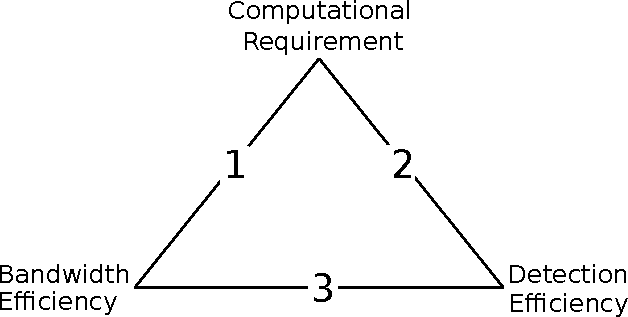
\includegraphics[width=0.5\linewidth]{img/edge_computing_vs.pdf}
	\caption{Comparison of the three event detection methodology across three metrics.
	Methods are as follows: naive method (2), self triggering (1), Napali, hybrid solution (3)}
	\label{intro:fig:edge}
\end{figure}
The naive method provides the best detection ability and the smallest node computation requirement.
However, it does so at the cost of the largest bandwidth consumption.
The self triggering method has the lowest bandwidth consumption of the three.
The disadvantage of this method is twofold.
First of all in order to maintain a high detection rate a reasonably low threshold for anomalies has to be used.
This may cause a large number of false positives due to local noise and sensor noise.
Secondly, global anomalies will often diminish in magnitude as a function of distance from the epicenter, thus far removed sensor nodes may completely miss events.
These low threshold events may be invaluable for reconstructing the dynamic of the anomaly propagation, however they will be missed by the detection algorithms.


Napali's hybrid approach provides the opportunity for much better anomaly detection rate and background noise rejection, by correlating the features that are computed on the sensor nodes.
Napali has moderate bandwidth consumption, however the bandwidth consumption is tunable since the features can be computed for varied temporal windows length of which can be adjusted in real time.
Napali does requires the highest sensor node computing power, since not only does it need to extract the triggering features from from raw data, it needs to maintain a buffer of sensor measurements to send to the sink if an anomaly is detected.

The downside of the Napali framework, is the requirement for two way communication between the sink and the sensor node.
In order to participate in event detection Napali sensors need to be able to both send raw and feature extracted data, as well as receive the control signals from the sink.
In contrast, the naive and self triggered approaches only require a one way link to send the raw data to the sink.
As such, standalone devices can be retrofired to participate in distributed event detection in the naive and self triggered approaches, while Napali requires custom devices specifically tailored for cooperative event detection.

I claim that there are several benefits to the Napali method compared to the naive and self triggered approaches.
\begin{enumerate}
	\item \textbf{Bandwidth usage is minimized:} Instead of sending the entirety of raw data, only extracted features are sent.
	This features will have a tiny fraction of the bandwidth requirement when compared to raw waveforms.
	Furthermore, the temporal window which encompasses a single feature can be adjusted in real time.
	Thus as soon as an anomalous behavior is observed in a subset of sensors, this window can be adjusted for a finer grained feature extraction.
  
	\item \textbf{Effects of latency are minimized:} Even at 1Msample/second at 16bits of resolution, the memory requirement to store 5 minutes of raw waveform without compression are on the order of 512MB, which is well within the realm of cheap single board computers.
	With compression specifically suited to the signal of interest, the memory requirement can be reduced even further.
	This gives the triggering stream sink plenty of time to respond to the anomalies in the data and request raw waveform from the monitoring devices.
  
	\item \textbf{Sink processing requirements are minimized:} Since most of the feature extraction is already performed at the device level the triggering stream sink computational resources can be minimized.
	With the advent of IOT, the computational capacity of the edge devices is quickly growing.
	Napali exploits these resources, and thus minimizes the sink computational requirements.
  
	\item \textbf{Sub-threshold data acquisition:} The triggering stream sink makes the decision to acquire raw waveform from sensor nodes.
	This allows researchers to collect data from devices which were only mildly affected or not affected by the disturbance.
	This provides new possibilities for investigation of disturbance propagation across the sensed area.
  
	\item \textbf{Power failure resiliency:} In the case of the complete power failure or communication blackout, if the monitoring device has a battery backup capability, each sensor has a record of the entire raw waveform leading up to the power interruption.
	Prior to shutdown the sensor node will transfer all of the raw data from the volatile memory to on-board permanent storage.
	Once the power or communication channel is restored, select portions of the buffer may be sent back to the data sink.
	This creates an additional layer of resiliency for the anomaly detection network.
  
	\item \textbf{Flexible Privacy:} Anomalies which were only observed at a single point are most likely local noise and pose little value for global state monitoring.
	It's up to the user to decide how to process disturbances which affect their sensor.
	For example user may choose to record a full waveform, only certain features, or record nothing at all.
	Secondly, if the saturation of the device is high enough only a subset of them would need to send a triggering stream for event detection, while the rest will be used for acquiring raw waveform for small temporal regions containing global events.
  
  \item \textbf{Temporal Locality:} By exploiting the temporal locality it is possible to ascertain the geographical extent of the anomaly with only coarse features.
  This allows for a simple robust algorithm which may be deployed at the sink node for anomaly detection.
\end{enumerate}

\section{The problem of power quality} \label{intro:sec:pq}
Power quality monitoring along with other smart grid domains is a field well suited for distributed sensor network monitoring.\cite{liu2017distribution} \cite{peisert2017lbnl} As the power grid moves from centralized generation with a few centralized power plants to distributed generation with residential power production, a distributed  consumer level monitoring system becomes ever more important.
Traditionally utilities do not monitor the quality of power besides the consumption beyond the substation level.
This is due to the fact that the last opportunity that the utility has to regulate and filter the grid voltage in the hierarchical power distribution is at the substation, or neighborhood level.
This methodology is unsustainable, as residential renewable energy production if not properly monitored and controlled will have an adverse effect on the overall grid stability.
Furthermore, lack of residential monitoring may lead to dangerous conditions such as islanding, where an otherwise powered down grid may have a small powered island sustained only by the unmonitored residential renewable generation.
Finally, residential power quality monitoring gives utility costumers an opportunity to evaluate the quality of power delivered to their household.
As consumer electronics are becoming more and more complex, they become more sensitive to the power anomalies.
Grid monitoring is traditionally the responsibility of the utility, however in most cases utilities only have to disclose power interruptions lasting several minutes.
Small interruptions, and partial interruptions such as voltage sags, swells, frequency fluctuations and transients will often go undisclosed by the utility and unnoticed by the consumer, but may cause premature failure in grid connected electronic devices.
It is in the best interest of the consumers to monitor the quality of the power that is delivered to them, meanwhile the same same monitoring system will also allows researchers and utilities to monitor the entirety of smart grid.

\begin{figure}[h]
	\centering
	\begin{subfigure}{.5\textwidth}
	  \centering
	  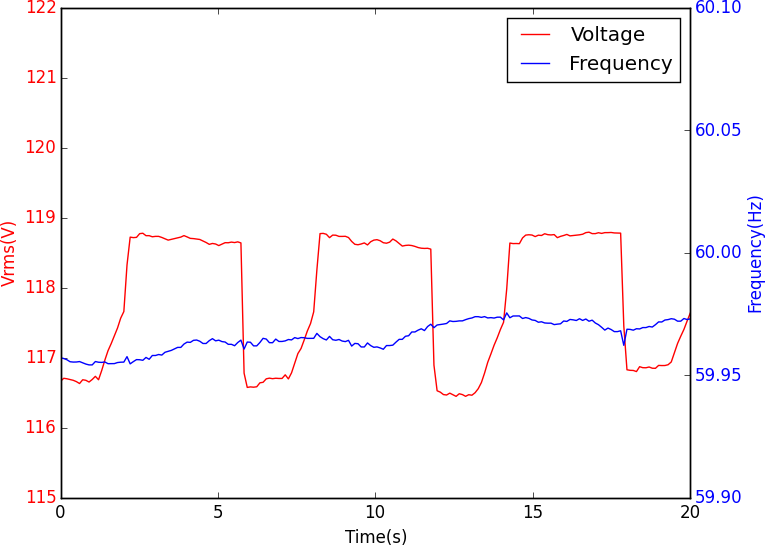
\includegraphics[width=0.9\linewidth]{img/hotplate.png}
	  \caption{Voltage signal produced by a hotplate.}
	  \label{intro:fig1:sub1}
	\end{subfigure}%
	\begin{subfigure}{.5\textwidth}
	  \centering
	  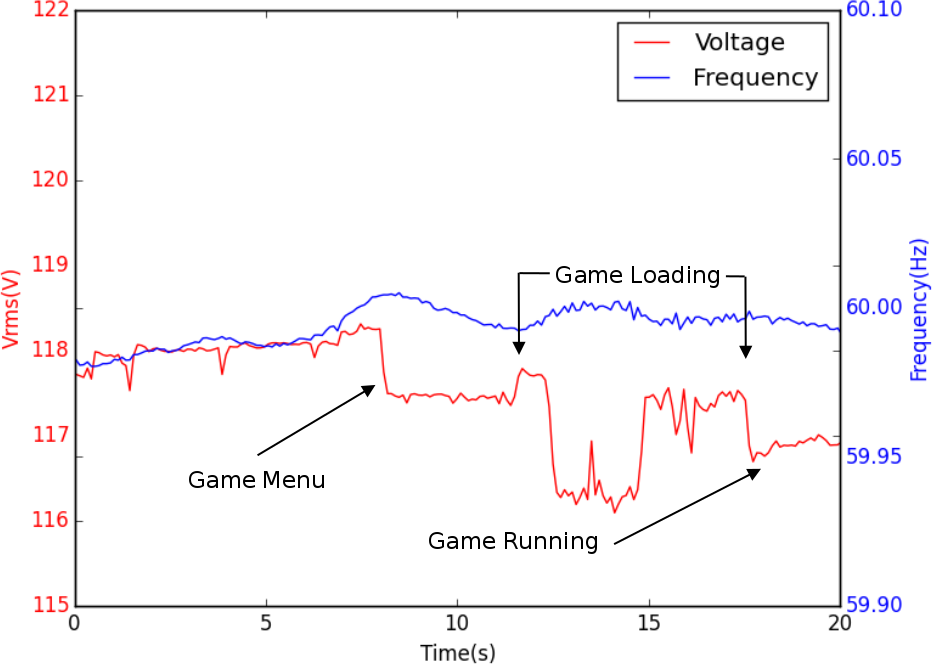
\includegraphics[width=0.9\linewidth]{img/PC.png}
	  \caption{Voltage signal produced by a desktop PC running a complex task}
	  \label{intro:fig1:sub2}
	\end{subfigure}
	
	\begin{subfigure}{1\textwidth}
	  \centering
	  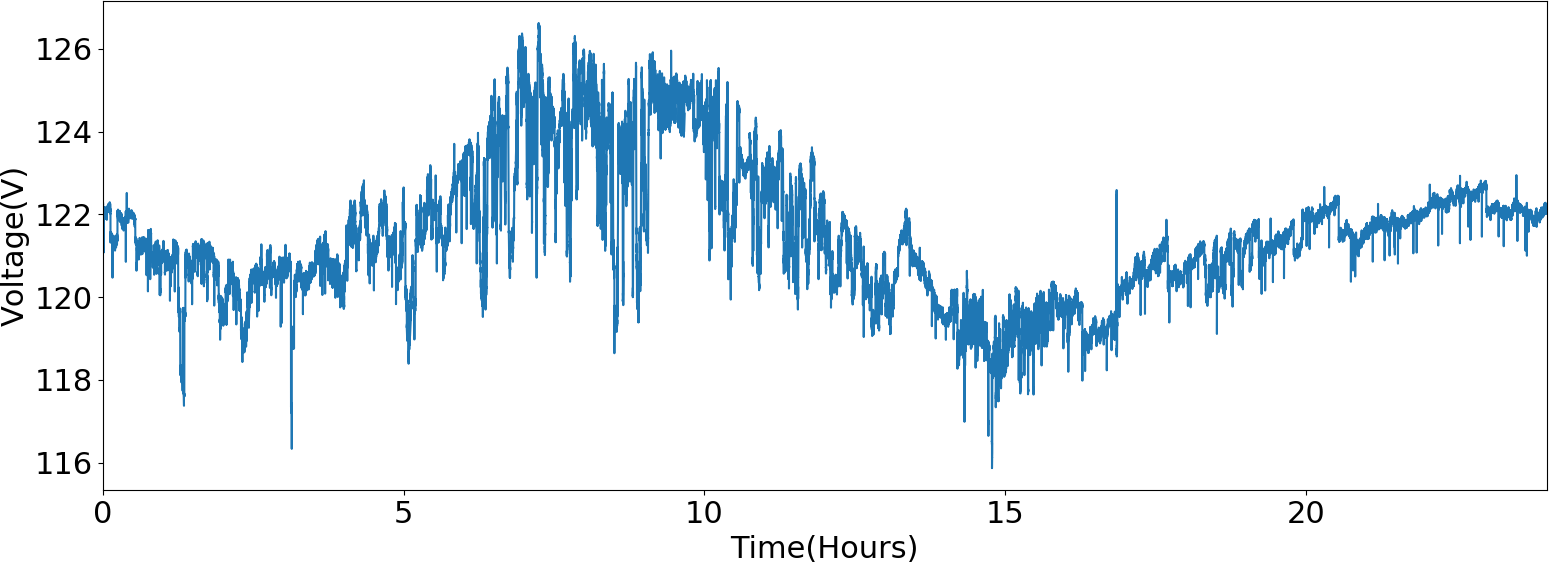
\includegraphics[width=0.9\linewidth]{img/johnson_daily.png}
	  \caption{Line voltage recorded over 24 hours in a residential household with photovoltaic installation.}
	  \label{intro:fig1:sub3}
	\end{subfigure}
	
	\caption{RMS voltage waveform generated form the consumer side of the meter under various conditions.
	All waveform were recorded using the OPQ Box 2.}
	\label{intro:fig:1}
\end{figure}

Residential power quality monitoring presents a number of issues.
First of all, it is difficult to discern which side of the utility meter a power disturbance came from.
Consider a voltage sag generated by a 1kW hot plate shown in Figure \ref{intro:fig1:sub1}.
 Since the output impedance of the power grid is non-zero a high powered device can cause a significant voltage sag affecting every device connected to the same circuit.
 Secondly, recoding the voltage waveform resulting from non linear load can result in privacy leaks for the end user.
 Consider the voltage waveform produced by a PC running a video game as shown in Figure \ref{intro:fig1:sub2}.
Throughout the game loading process the power load varies based on which components are in use.
Furthermore, regions with CPU load, harddisk load and video card load can be readily identified by measuring the resulting voltage sag.
Recording these event's has an adverse effect on end-users privacy and offers no immediate benefit in studying grid stability.
Finally distributed power generation such as rooftop solar has significant effect on the residential voltage waveform.
Consider the voltage waveform shown in Figure \ref{intro:fig1:sub3}.
This waveform was recorded over 24 hours in a household with a rooftop photovoltaic installation.
Similar to the voltage sag case since the power grid impedance is non-zero residential power generation will cause a voltage swell during peak hours of sunlight as evident by the waveform.
Combined with the global voltage sag during hours of peak demand (3pm) combined with the lack of PV production during that time, photovoltaics installations can result in a daily $10V_{rms}$ swing.
Residential power quality monitoring can be accomplished via a distributed sensor network made up of power quality monitoring devices with high degree of penetration across the end points of a power grid.
Furthermore, in order to monitor the dynamics of the entire power grid via residential line voltage monitoring it is imperative to monitor across multiple locations simultaneously.
This combined with temporal and spatial correlations of data produced by the sensors allows for identification of grid wide anomalies without a high rate of false positives.
Additionally, not all power quality events affect the entire grid, due to the hierarchical structure of the power distribution.
The final requirement for grid-wide monitoring is a novel distributed event detection system.

\section{Edge computing approach to power quality monitoring.}\label{sec:edge-computing-approach-to-power-quality-monitoring.}

IEEE1159 standard describes the techniques for single location power quality monitoring.
For transient monitoring it suggests a sampling rate of at least 7680 samples/second, up to 1 Megasample/second.
This implies that if a power quality event detection system relies on raw data from all monitors it would do so at a very large bandwidth cost.
At 20 Ksamples/second at 16bit per samples a single monitoring device would generate 300Kb/second.
Several thousand devices could easily saturate at 1Gb link with no obvious benefit.
Collecting and recording all of the raw waveform data from residential power quality meters for batch processing presents some privacy concerns as outlined above.
On board event detection methodology allows the measurement devices to select which temporal regions of measurements constitute an event.
This is a perfect strategy from the consumer's perspective, since it would allow for recording of power quality information which directly impact their residence.
As mentioned in Section \ref{intro:edge}, this method relies on a threshold based approach where every device has a computes several metrics from the raw waveform and compares then to preprogrammed threshold values.
Metrics such as $V_{rms}$, fundamental frequency and THD are easily adapted for single point power quality measurements.
Temporal regions during which these metrics surpass a threshold are considered by the device as a power quality event, and thus are recorded.


The problem with the method outlined above is that grid-wide power quality events do not affect the entire grid in the same way.
For example due to the grids hierarchical structure a voltage sag on one sub-circuit can manifest as as a sag of a different magnitude or even a swell on another.\cite{kahle2016power} This may result in a situation where some of the monitoring devices will not consider a power quality anomaly as an event, because it did not surpass the metric threshold, and simply ignore it.
From the research perspective, however, it is important to get raw data from all of the affected devices not just the ones that were the most affected.
This makes a hybrid centralized/decentralized event acquisition strategy more attractive for distributed residential power quality monitoring.
In this scheme all monitoring devices use local processing resources to feature extract the incoming waveforms while storing them locally for several minutes.
A sink collects all of the extracted features and looks for anomalies which are present in the feature data stream which we will refer to as triggering stream.
If an anomaly is present in only a single device, it is highly probable that the disturbance occurred in the residence.
Depending on the user's privacy preference, raw data for a single device anomaly can be be recorded for later analysis, or in case of a highly privacy conscious user, ignored.
On the other hand if the triggering stream shows an anomaly temporally collocated across multiple devices, the entire network or a subset of the network may be queried for raw waveform data for a temporal region which corresponds to the disturbance in the triggering stream.

The main disadvantage of this method is that while there are plenty of power quality event detection methodologies for single location, there has been little development in the distributed event detection methods and metrics.
Two problems are quite similar, indeed one may use the same metrics for distributed event detection as with the single point power quality monitoring.
However, it's also important to consider temporal locality of anomalies detected across multiple devices and effects of device synchronization.
Power quality anomalies such as voltage sags and transients will propagate through the transmission lines at the speed of light, however due to the non-linear elements which make up the power-line junctions, a certain temporal spread in event detection across multiple locations is expected.
For large power grids such continental United States grids, large frequency fluctuations propagate in a highly nonlinear ways.
In these cases the event propagation is limited by the inherent rotational inertia of the power generation systems, and the speed at which the grid protection elements such as reclosers and circuit breakers operate.
Regardless, the closer local anomalies are detected in time, the more likely are they to be a result of a gridwide event.
Unfortunately, it is unfeasible to perfectly temporally synchronize the distributed power quality monitors.
While methods such as GPS can in principle provide synchronization of up to 10ns jitter across a large geographical region, they require a line of sight to the sky, and add a non-trivial cost to the bill of materials for every power quality meter.
Furthermore, GPS is prone to losing signal depending on atmospheric conditions, and can be very sensitive to fluctuations in the power supply voltage, a critical time in power anomaly detection.
An alternative to GPS is Network Time Protocol.
Network time protocol can provide timing synchronization on the order of $~10ms$ across Internet, which is on the order of $\frac{1}{2}$ of a grid cycle.
NTP performance could be further improved by using geographically close time servers which are themselves synchronized via GPS. Consider a situation where two devices are located in household which experience a local $100ms$ power quality disturbance every $10$ minutes.
Even with a $~10ms$ synchronization jitter, it will take on average $21.5$ days before the two disturbances are observed within $20ms$ of each other.
If a third device is introduced, it is highly unlikely that all 3 would observe unrelated local anomalies within $20ms$ of each other over the lifetime of the power quality monitoring network.
This implies that combination of temporal and threshold based correlation on the feature extraction data would allow one to build a robust residential based power grid monitoring system which would yield a very low rate of false positives.

\begin{figure}[h]
	\centering
	  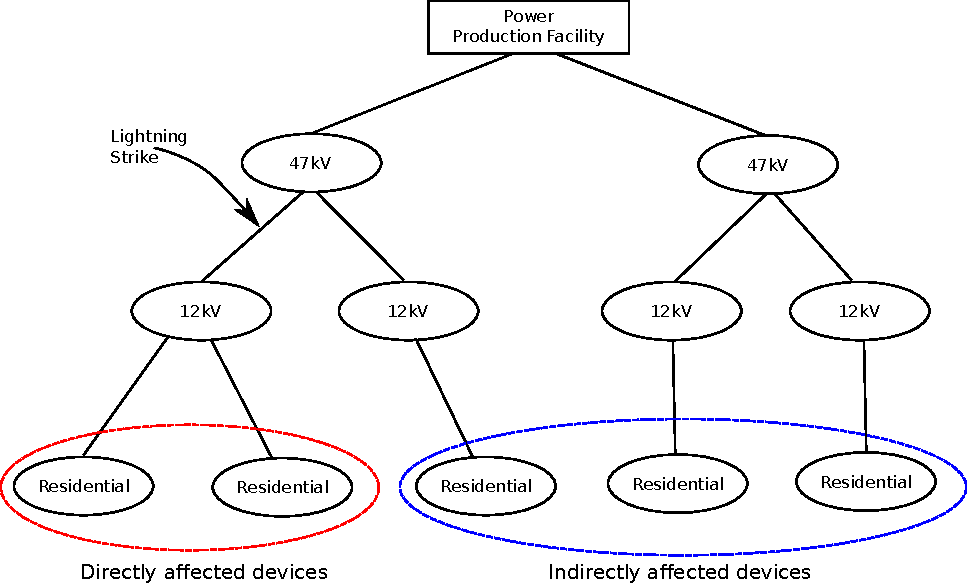
\includegraphics[width=0.9\linewidth]{img/grid_hierarchy_cartoon.pdf}
	  \caption{Power quality anomaly propagation example.}
	  \label{intro:fig2}
\end{figure}

\section{Thesis claim and evaluation} \label{intro:sec:claim}

Today's big data world is plagued with the issues of data cleaning and validation, even though it's being relied on for timely, accurate and actionable intelligence.
With large ingress of unstructured data these issues are unavoidable, and preprocessing will remain a large portion of the analysis workload.
However, in the case of sensor networks designed for a specific purpose, the tasks of anomaly detection can be pushed to the edge of the network using the Napali methodology.
The claim of this thesis is that Napali provides novel architecture that is both a feasible solution to the problem of distributed power quality monitoring and which also provides significant benefits over the two standard alternative architectures (all computation/storage at nodes, all computation/storage at the sink).

To evaluate the feasibility of the Napali framework, I propose to implement it as part of the Open Power Quality(OPQ) system and apply it to the problems of power quality monitoring.
Combined with higher level anomaly analysis, Napali provides important services for a Open Power Quality power quality monitoring network.
This network is made up of a group of monitoring devices as well as a centralized data sink server.
This system will be deployed for testing at the University of Hawaii at Manoa campus, by deploying power quality monitors across at least 20 buildings on campus.
The University of Hawaii at Manoa campus is a unique testbed for such a network, since entire campus is isolated to its own microgrid, connected to the municipal Oahu grid via a 46kV feeder.
Furthermore, the University of Hawaii has deployed a set of smart power monitors at the key positions in the grid, which can be used as a state of the art ground truth for evaluation of OPQ performance.


The system relies on a custom residential power quality monitor called OPQ Box, designed specifically for distributed monitoring using the Napali framework.
Instead of performing local analysis on the voltage waveform with the aim of PQ anomaly detection, or forwarding all the recording measurements to the centralized sink, OPQ boxes computes a small subset of features on the input voltage waveform.
These features are then forwarded to the Napali framework's centralized sink which performs the anomaly detection on reduced data, while the raw waveform is retained for a short time on the OPQ Box.
If the sink determines that a possible anomaly has occurred, a request is sent to the affected and nearby devices for raw data.

The goal of Napali is not to provide a low rate of false positives for a particular type of a power quality disturbance.
Indeed, once the raw data is acquired by the sink, filtering through the potential anomalies is trivial using well established methods.
Instead, the focus of my detection system is balancing low bandwidth required for detection with the low rate of false negatives.
Furthermore, monitoring at the leaf edges relies on the hierarchical nature of the power grid in order to ascertain the state of the entire power generation and delivery system.
As noted in the literature, power quality disturbances tend to propagate down the hierarchy as shown in Figure \ref{intro:fig2}.


Consider a lightning strike on a hypothetical 12kV feeder line in a hierarchical power grid.
The directly affected devices will be the ones downstream from the disturbance.
These devices will experience the most severe effects, most notably transients, as they propagate throughput the power delivery infrastructure.
The indirectly affected devices will expedience a power anomaly mainly attributed to the power production entities trying to compensate for the large disturbance caused by the lightning strike.
Thus, monitoring of the leaf edges of the power delivery system can in principle provide insights into the disturbances that originate deep inside the power distribution network.

The Open Power Quality system is designed to be a test bed for development of new power quality detection and analysis algorithms.
Its introduction will facilitate development of new techniques and methods for studying power system, by utilizing the Napali framework as the main anomaly detection methodology.
To evaluate the benefits of this architecture, I will assess the data collected by the OPQ network at the University of Hawaii in order to determine if the claimed benefits of the architecture are observed in practice.
The description of the evaluation processes for the benefits described in Section \ref{intro:section:napali} are summarized below.

\begin{enumerate}
  \item \textbf{Bandwidth usage is minimized:} Bandwidth consumption of the OPQ system will be carefully monitored, recorded and compared to the bandwidth required to transmit the equivalent amount of raw data.
  A more detailed description of this evaluation can be found in Section \ref{iexp:sec:band}.
    
	\item \textbf{Effects of latency are minimized:}  Latency limits of the triggering system will be examined.
	Since these are heavily dependent on the raw data storage ability of the OPQ Box, latency effects will be tested under various amount of memory allocated for this task.
	A more detailed description of this evaluation can be found in Section \ref{iexp:sec:lat}.
  
  \item \textbf{Temporal locality:} Data acquired from the UH building level meters will be compared with the data acquired via the Napali triggering framework.
   This will allow me to establish the rate of false positives and negatives and evaluate the temporal locality triggering algorithm.
   Furthermore, the single location events, which are normally rejected by Napali will also be examined and compared to the data provided by the building power meters.
   A more detailed description of this evaluation can be found in Section \ref{iexp:sec:loc}.

  \item \textbf{Sink processing requirements are minimized:} Synthetic benchmarks will be carried out on the sink node to determine the scalability of the triggering system.
  These scalability metrics will be compared with a synthetic benchmark of running multiple copies of the OPQ Box analysis software on the same node.
  This will allow me to compare the scalability of the sink node in the case of sending the entirety of raw data stream versus the Napali frameworks approach of only sending extracted metrics.
  A more detailed description of this evaluation can be found in Section \ref{iexp:sec:scale}.

	\item \textbf{Sub-threshold data acquisition:} Evaluation of the sub-threshold data acquisition will performed in two ways.
	First, the triggering stream from the OPQ Boxes will be stored along with the acquired raw data.
	The triggering stream can be used to compute which fraction of devices would have self triggered if operating autonomously.
	Next the building level meters self triggering capabilities, will be compared to the Napali, sub-threshold triggering in order to compare Napali to a commercially deployed system.
	A more detailed description of this evaluation can be found in Section \ref{iexp:sec:sub}.
  
\end{enumerate}
Although power failure resiliency and flexible privacy are claimed benefits of the Napali architecture, they will not be evaluated as part of this thesis research.
Flexible privacy would require a much larger deployment, and a user study, which is beyond the scope of this project.
Furthermore the power failure resilience of the Napali framework would require a significant development effort in development of the battery management system.
Since complete power failures are quite rare, there is no guarantee that a single power outage would occur at the UH campus during the deployment.


The last claim of this dissertation is that the Napali architecture can be applied to other domains.
Once the Napali framework is fully characterized, and its strengths and weaknesses are well understood, I intend to perform an in-depth literature review of other domains which could benefit from Napali-like approach to event detection.
I will also characterize the kinds of design changes to existing sensors that the Napali Framework will require in order to apply it to these domains.



\chapter{Related Work}

\section{Edge computing}\label{sec:lit:edge-computing}
Projections performed by Forbes suggest that by 2025, more then 75 billion Internet of Things(IOT) devices will be connected to the Internet.\cite{forbesiot}
As the devices at the edge become more computationally capable and more numerous, it becomes imperative to share the computational load not only across the cloud services, but across the devices themselves.
Furthermore, a large portion of these devices, such as home automation, do not require a connection to the cloud in the first place.
Instead they require a connection to the edge IOT hub, or need the cloud service only to establish or broker communication with another IOT device.
Edge computing is a subset of IOT research, which concerns itself with distributing the computational load across the devices at the edge of the of the network. \cite{satyanarayanan2017emergence}
\begin{figure}[h]
    \centering
    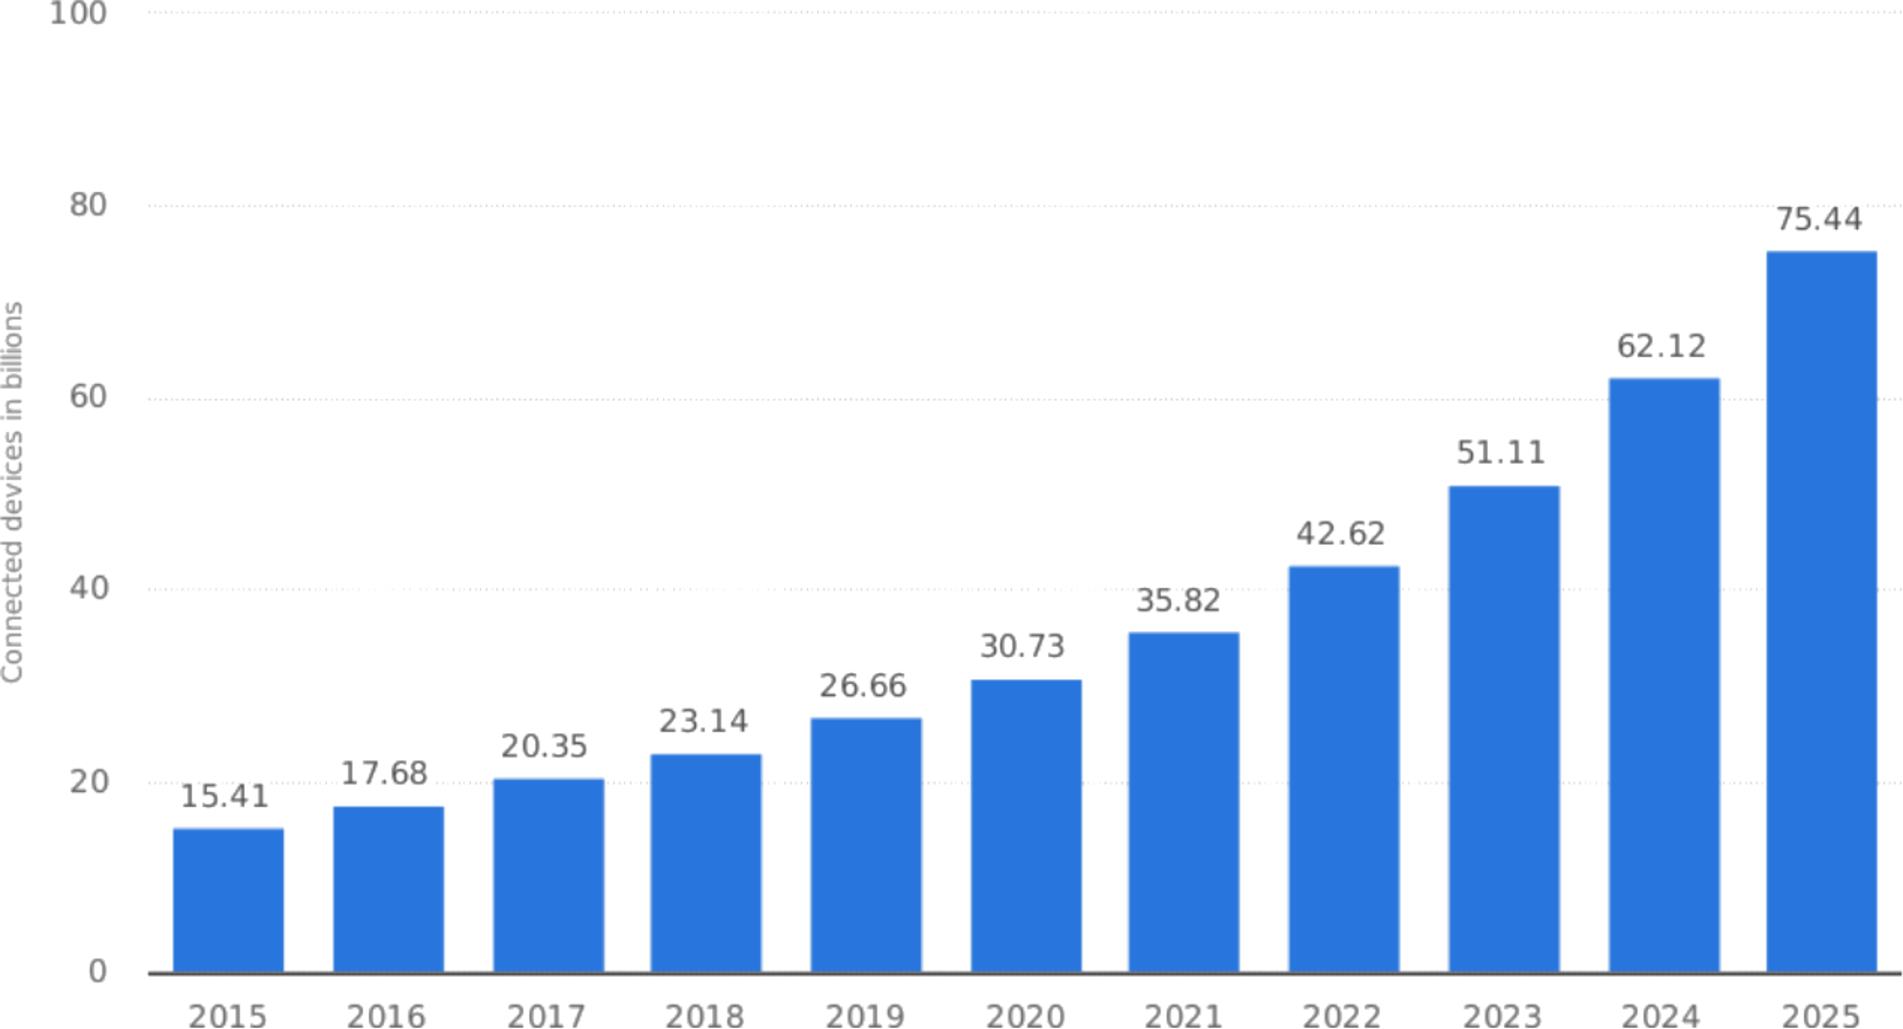
\includegraphics[width=0.8\linewidth]{img/iot_statistics.pdf}
    \caption{Projected number of IOT devices worldwide.\cite{forbesiot}}
    \label{lit:fig:1}
\end{figure}

This change in computational strategy may seem inconsequential at first.
However, upon deeper reflection it becomes clear that this is a major paradigm shift which brings IOT closer to the sensor network world it is often compared with.
While pioneering work in IOT always assumed a one or two-way communication between the IOT device and the cloud service, utilizing TCP/IP as an end-to-end protocol, it is becoming clear that this approach is unsustainable, and is often undesirable.
This communication model has clear disadvantages in wasted communication, computation, and privacy.
Furthermore, the rigid computation communication model is not flexible enough to support devices which are beyond the edge of the TCP/IP network without resorting to ad-hoc routing. \cite{gagliardi2011content}

The first attempt to address the bandwidth and latency issues arising with widespread IOT adoption came in form of content delivery networks (CDNs).\cite{gagliardi2011content}
CDNs circumvent the generic cloud information delivery problems by placing transparent caches geographically spread across the application domain as shown in Figure \ref{lit:fig:2}.
When a user or an IOT device makes a request for an object, this request is forwarded to the nearest CDN node for processing.
If the node contains the object in its cache it is immediately forwarded to the requestee.
Otherwise a request for the object is forwarded to the centralized cloud data store, and returned to the requesting device, as well as placed in the local cache.
This approach has the advantage of moving the data closer to the end user, thus reducing latency, and taking advantage of geographical locality.
Another advantage of this method is the added resiliency of the CDN architecture to a single point failure.
If a local cache node fails, its userbase can be forwarded to another node, although incurring additional latency.
Additionally, if a centralized data store becomes unreachable, the local cache nodes can to some extent mask it's outage by forwarding the data available locally.
This approach does have some drawbacks.
While it makes it easier to enable faster transactions regarding data, it is not trivial to move application logic to the local cache nodes.
Furthermore, the CDN methodology, still relies on a central mediator for device communication, even if the devices are located in the same room.

\begin{figure}[h]
    \centering
    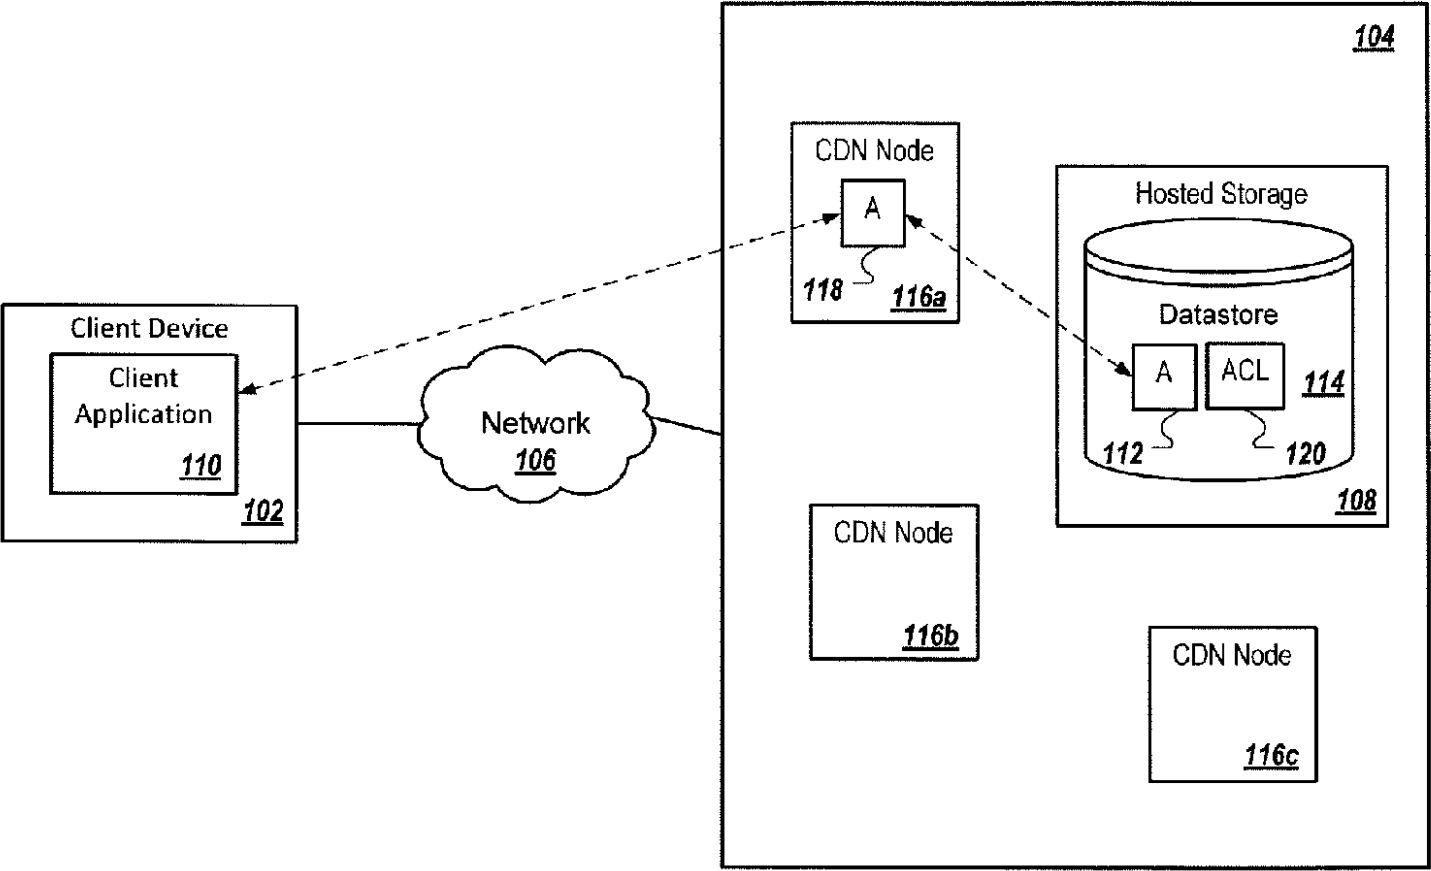
\includegraphics[width=0.6\linewidth]{img/cdn.png}
    \caption{Content delivery network architecture.
    As described in the Google pattent.\cite{gagliardi2011content}}
    \label{lit:fig:2}
\end{figure}

In an attempt to support a more diverse IOT ecosystem, current research is focused on moving the cloud service ever closer to the edge of the network.
Since the majority of IOT devices are located withing one hop of the Internet, the next logical place to locate a content provider is at the wireless basestation.\cite{satyanarayanan2017emergence} These servers, commonly referred to as cloudlets or fog servers, are collocated with various wireless basestations, which allows them to provide a location specific service to the user without using the Internet.
This approach also provides uniform access and simplifies intercommunication between a variety of devices, including those that don't use TCP/IP. Unlike the localized cloud cache approach relied on by the CDNs, fog servers are built with the notion of moving not only data but also the application logic to the edge of the network.
To facilitate inter-device communication between the devices using differing wireless protocols, fog servers can no longer rely on TCP/IP routing.
Instead, TCP/IP becomes yet another transfer protocol along with Bluetooth, Zigbee, 3g etc, with routing between the devices implemented as a software service.\cite{edgeiot} A few use-cases of such technology are already found in industry.
Examples of these include airline/bus in-flight entertainment, and shopping mall directory apps.
A block diagram of this infrastructure is shown in figure \ref{lit:fig:3}.
In the future, emerging technologies which are sensitive to latency, such as virtual and augmented reality will benefit from fog computing, since it's inherently lower latency then the cloud counterparts.

\begin{figure}[h]
    \centering
    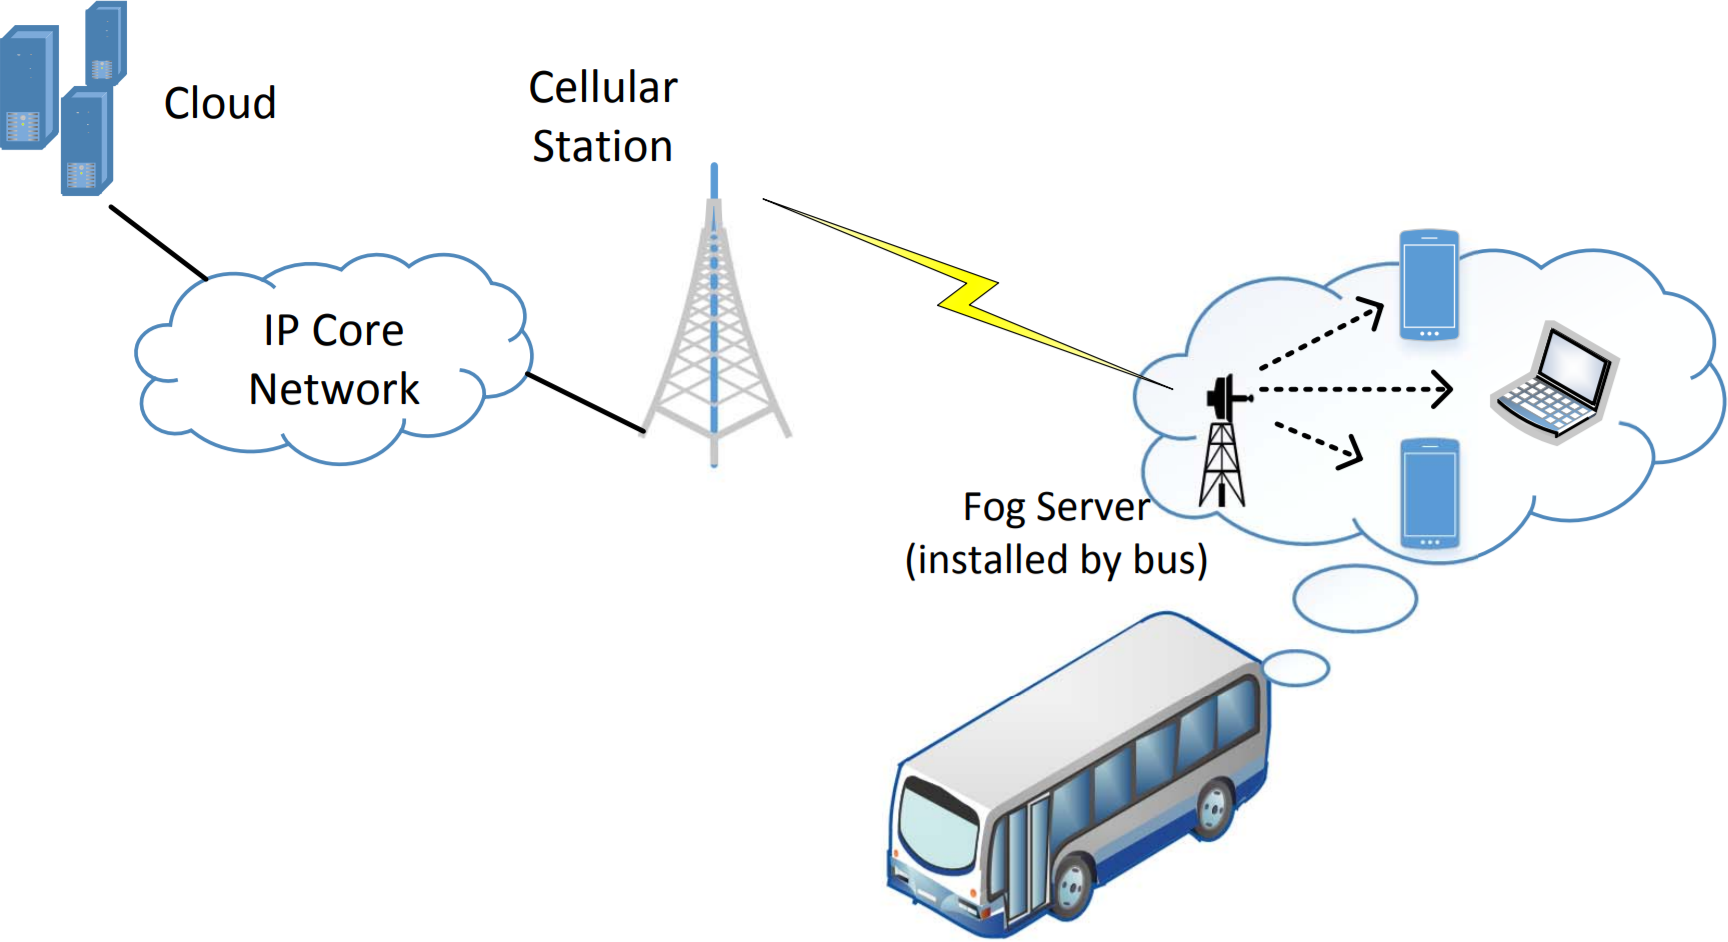
\includegraphics[width=0.6\linewidth]{img/fog_comp.png}
    \caption{Fog computing use in transportation.
    The bus cloudlet provides a cache for common data such as commuter schedules and traffic information, while routing other queries to the Internet.\cite{edgeiot}}
    \label{lit:fig:3}
\end{figure}

With the architecture for low latency communication between the edge devices and the fog provider established, the state of the art in edge computing research is focused on intelligent sharing of the computational resources in the fog system.
Edge servers generally have far more computational capacity then the edge device, however, they service many such devices.
Additionally, due to the fickle nature of radio links connecting the edge device to the fog service, the work sharing protocol must be able to cope with link and packet loss.
Finally, in the case of battery powered devices, the energy cost of transmitting the computational job, and receiving its result may exceed the cost of performing the computation locally.
Finally, with mobile edge nodes, such as smart phones, and smart cars, computational offloading algorithms must be able to handle constant network reconfigurations as the edge nodes enter and leave the fog server geographical area.
A number of algorithms have been proposed for efficient and robust computational sharing in fog environments. \cite{oueis2015fog} \cite{wang2015mobiscud} \cite{wang2013mobile}

Napali fits in-between the CDN and Fog server architectures.
The power quality disturbances are generally localized to a specific area, so a sink placement which covers a small geographical area are preferred in order to reduce latency and reduce unnecessary communication with the centralized cloud location.
Furthermore, sink-driven measurement rate allows the OPQ Box to dynamically scale the computational and communication overhead.
Finally the event, classification and analysis are similar to the computational offloading strategies currently under development in the edge computing field.

\section{Distributed Power Quality Monitoring}\label{sec:distributed-power-quality-monitoring}

Power quality monitoring is a long established field in the smart grid domain.
However, the vast majority of research so far has focused on single point power quality monitoring.\cite{silva2017development} Such research has extremely useful applications in industry, since it allows one to ascertain the absolute quality of the delivered power at a given location.
However, since power quality disturbances can originate both from local sources and from gridwide disturbances, single point monitoring is not particularly useful for smart grid research.
Several projects have developed a distributed approach to power quality monitoring, the most prominent being the FNet project and the Power Standard Lab PQube deployment.


The FNet project designed, manufactured and deployed a Phase Measuremnt Unit (PMU), across over 300 locations across the united states.\cite{zhang2010wide} PMU devices plug into an outlet, and sample the power line voltage at the rate of about 1.5kS/s.
The sampling is disciplined by GPS, and as such FNet devices are extremely sensitive to voltage frequency and phase angle.
The precision of the FNet devices is $~0.5mHz$ for frequency and $0.02^{\circ}$ for phase angle.
Collected data is sent to the collection service at 100ms intervals via the Ethernet connection.
Using these devices FNet was able to observe several large power disturbances in the US power grid.
The robustness and sensitivity afforded by the GPS receiver makes this project an excellent source of frequency data across large geographical area, however, the sampling rate of 25 samples per grid cycle is far too low to properly sample fast transients and sags.
Furthermore, FNet provides no methodology for acquiring raw data for event disturbances which it records.

Power Standards Lab (PSL) has been an industry leader in power quality monitoring, and has authored several standards on the topic.
Furthermore, PSL has developed and deployed a large number of power quality monitors called PQube across the world.
The exact number of deployed devices is uncertain since a lot of the devices are deployed industrially and are not available to the public.
However PSL has several publicly available devices, as well as several PQ datasets accessible for smart grid researchers.
PQube devices are an industry standard for power quality monitoring, sampling at $12.8kSps$ for both the voltage and current waveforms.\cite{pqube_spec} Each PQube device is supplied with a NIST certificate of compliance and complies with the IEC 61000-4-7:2002 standard for PQ measurements.
Incidentally, this standard was authored in part by the PSL staff.
Similarly to the FNet PMU, PQube devices are GPS disciplined, additionally the sampling is phase-locked to the voltage waveform allowing for an even more precise metric extraction.
Finally each PQube device is configurable with custom thresholds which allow it to record raw PQ event data for the location it's monitoring.
PQube offers a centralized data collection option with flexible communication schemes ranging from Ethernet to Cellular.
Since PQube devices monitor current in conjunction to voltage, its installation requires it to be placed into the electrical box of the target, by a licensed electrician.\cite{von2014micro} Furthermore, the GPS synchronization requires addition of extra conduit to the electrical box to allow for an antenna.
Finally, since the PQube devices are designed for single location measurements, distributed event detection using the PQube network is particularly difficult, with a lot of low magnitude gridwide events being incomplete or missing.


Unlike the single point monitoring solutions, the Napali framework is incapable of operating as standalone PQ monitor without a cloud sink.
Furthermore, even with the event detection sink, the goal of Napali is to reject local anomalies in order to reduce the communication and computational overhead.
While not as sensitive as the PQube device, the deployment price per unit is two orders of magnitude lower, while providing better sensitivity then compared to the FNet device, when running with GPS.
The ability of OPQ Box nodes to utilize NTP, with WIFI connectivity, means that the OPQ Box deployment is much simpler then the FNet and PSL offering, without requirements of a clear view of the sky or additional wiring for Ethernet and GPS antennas.
Finally, Napali distributed event detection system allows for acquisition of the entirety of the PQ disturbances including in locations where the disturbance has been greatly attenuated by the electrical distance.
Thus, Napali is able to provide a more complete picture of the disturbance propagation throughout the smart grid.

\section{Anomaly detection in Power Quality Monitoring Networks.}\label{sec:anomaly-detection-in-power-quality-monitoring-networks.}

Anomaly detection in PQ monitoring networks remains an active topic of research.
The goal of PQ event detection is to isolate the temporal regions where the voltage or current waveform deviates from the nominal by a given threshold.
In some cases the aim is simply to notify a higher level control system in a realtime manner that a disturbance is taking place.
In other cases, the goal is to acquire the raw disturbance data for off-line analysis.
Most of the detection methods rely on statistics and thresholding in order to detect PQ disturbances.
Most of the literature concerns itself with single point detection, for purposes of protection of equipment downstream.\cite{gu2004statistical}\cite{karimi2000wavelet} \cite{shin2006power} Distributed power quality projects will generally utilize single single point detection across multiple devices in order to reconstruct gridwide propagation.\cite{von2014micro}

With a wide deployment of smart meters, PQ researchers gain access to a networked platform which is perfectly positioned for PQ monitoring.\cite{hoglund2012using}
The major issue for smart meter real time monitoring is bandwidth constraints.
Smart meter deployment is envisioned to communicate via a mesh network with a stationary or mobile base station used for data aggregation.
As such the bandwidth and connectivity is limited, thus requiring methodology which is capable of event detection in such environments.
Generalized local likelihood ratio detection is one method for overcoming these limitations.
This approach requires only a single bit to be forwarded from each smart meter indicating whether a disturbance is taking place or not.
These bits are aggregated at the ``master'' meter, and if their sum exceeds a threshold a higher level control system is notified of the ongoing disturbance.\cite{li2016cooperative} This approach is resilient to bandwidth limitations, and communication instability, however tunning thresholds for each individual meter requires a significant manual effort.

Systems designed for distributed PQ event detection using custom meters are prevalent in literature.
A study at CERN utilized PQube devices with gapless recording which were later analyzed off-line, in order to ascertain the propagation mechanics of PQ events.\cite{kahle2016power} In a realtime domain Shang Li and Xiaodong Wang extended their work in \cite{li2016cooperative} from smart meters to standalone devices, again advocating for single bit statistical based triggering generated by asynchronous meters.\cite{li2013monitoring} Unfortunately their work has never been verified beyond simulation.
The Transimeter project utilized an analog hardware event detector comprised of a high pass filter and a comparator for transient detection.
These devices had two data paths for the voltage waveform, one to the National Instruments DAC board, one to the hardware trigger circuit.
If a trigger circuit detected a transient, a flag was set on the NI DAC, which would in turn instruct the connected PC to send the data to the central server.\cite{daponte2004transientmeter} Unfortunately, the lack of cooperative detection and an inflexible trigger circuit makes this approach unappealing for modern power quality monitoring.
Some of the more exciting work in PQ detection is modeling the most efficient placement of PQ meters in order to provide complete coverage for the power grid. \cite{won2006new} Another is using distributed detection for localization of the event source.\cite{parsons1998direction} \cite{polajvzer2017evaluation}

Napali differs from the smart-meter approach in the use of WiFi for communication, which greatly decreases the communication constraints of the system.
Since the OPQ Box is always connected to the power grid it is monitoring, power concerns are minimal.
This allows Napali to implement more robust computational and communication strategies, not commonly possible with smart meter PQ monitoring.
Since the triggering stream is generated in software, it is possible to switch the detection metrics without redesigning new hardware.
Napali combines both cooperative PQ event detection and PQ event acquisition which makes it useful for future PQ event localization, and propagation research.\cite{parsons1998direction} \cite{polajvzer2017evaluation}


\chapter{Open Power Quality}
\begin{figure}[h]
  \begin{center}
  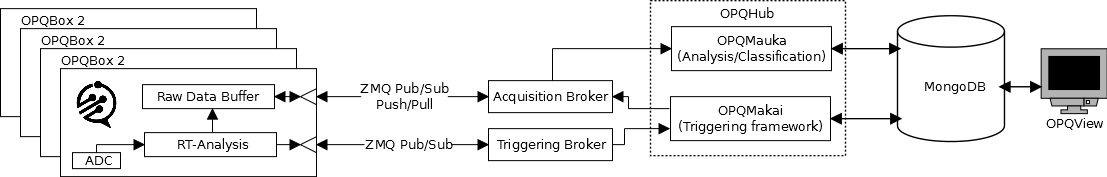
\includegraphics[width=0.9\textwidth]{img/system-diagram.png}
  \end{center}
  \caption{Block diagram of the OPQ Power Quality monitoring system.}
  \label{fig:opq:1}
\end{figure}

Open Power Quality (OPQ) power quality monitoring network utilizes residential power quality meters, called OPQ Boxes, in order to detect anomalies in the electricity distribution across the Oahu power grid.
In addition to OPQ Boxes, the OPQ project utilizes cloud-based aggregation services for power quality event detection, classification and display.
The block diagram of the OPQ network is shown in Figure~\ref{fig:opq:1} .

The major components of OPQ are:
\begin {itemize}
	\item OPQ Box: an in-house designed, open source power quality meter that conforms to Napali Framework requirements for the "source".
	\item Makai: data aggregation and event detection service that conforms to the Napali Framework requirements for the "sink"
	\item Mauka: event analysis and classification service.
\end {itemize}

The following sections describe the OPQ network components, services and protocols.

\section{OPQ Box}\label{sec:opq-box}

OPQ Box is an in-house designed power quality meter which focuses on providing the means for cheap, extensible and accurate residential power quality measurements.
The block diagram of the current revision of OPQ Box, OPQ Box2 is shown in the Figure~\ref{fig:opq:1:1}.
A complete device in an acrylic enclosure is shown in Figure~\ref{fig:opq:1:2}.

\begin{figure}[h]
	\centering
	\begin{subfigure}{.5\textwidth}
	  \centering
	  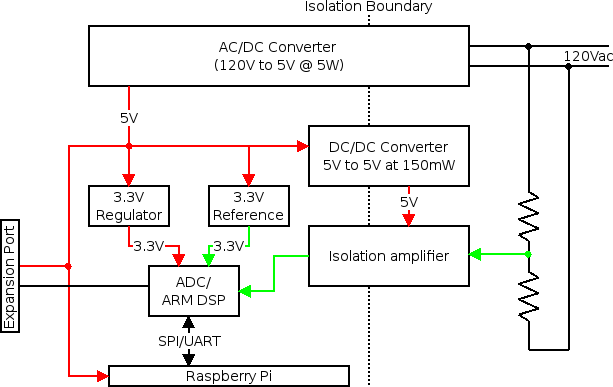
\includegraphics[width=0.9\linewidth]{img/opqbox_diagram.png}
	  \caption{OPQ Box2 Block Diagram.
	  The power path is in red, signal path is in green and the digital IO is in black.}
	  \label{fig:opq:1:1}
	\end{subfigure}%
	\begin{subfigure}{.5\textwidth}
	  \centering
	  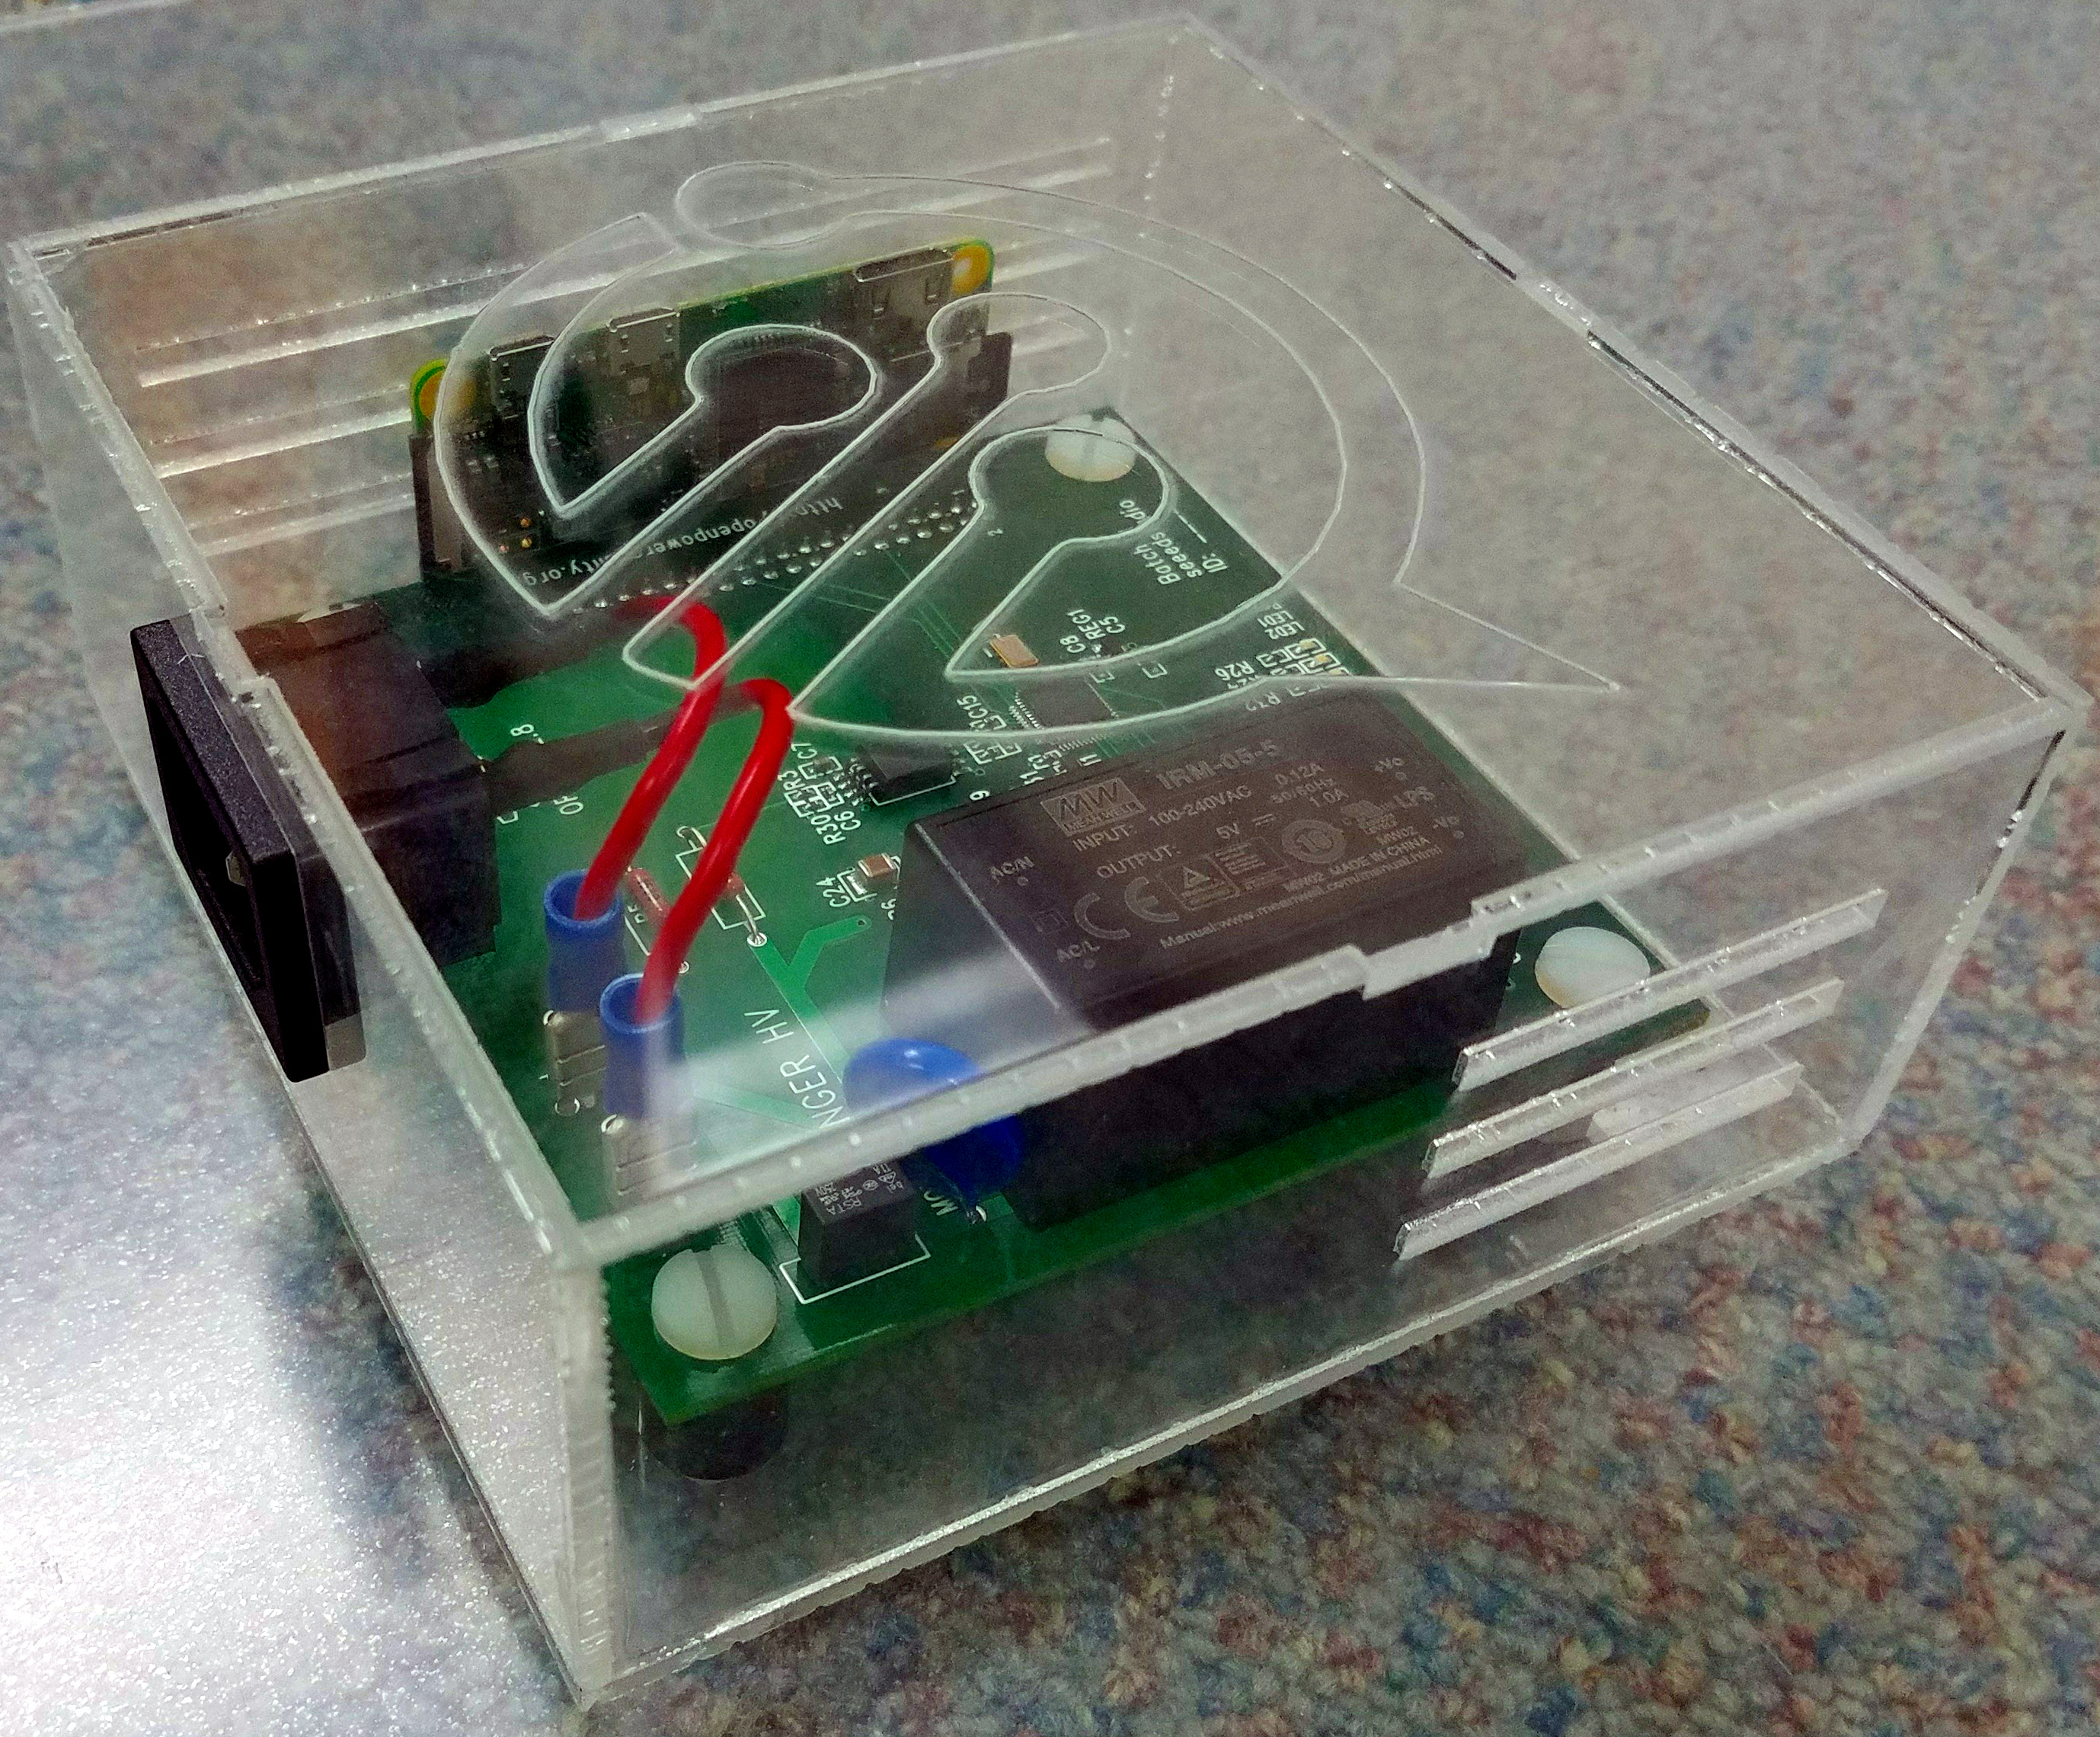
\includegraphics[width=0.7\linewidth]{img/opqbox_photo.jpg}
	  \caption{OPQ Box2 in an acrylic enclosure.}
	  \label{fig:opq:1:2}
	\end{subfigure}
	\caption{(a) OPQ Box2 block diagram and (b) production OPQ Box ready for deployment}
	\label{fig:opq:2}
\end{figure}

\subsection{Hardware}\label{subsec:hardware}

The power system of the OPQ Box2 electrically isolates most of the device from the AC mains power.
An isolated AC-DC converter generates $5V_{dc}$ from the mains $120V_{ac}$.
5V is used to power the Raspberry Pi, equipment connected to the expansion port, 3.3V regulators and voltage reference and an isolated DC/DC converter.
3.3V is used to power the isolated end of the isolation amplifier as well as the STM32F3 analog to digital converter/digital signal processor (ADC/DSP).
The hot side of the isolation amplifier is powered from the isolated DC/DC converter.
This allows OPQ Box to function with the battery attached to the expansion port, so that it may retain data and continue to operate during a power outage.


The analog signal path of the OPQ Box2 is complicated by the fact that the STM32F3 ADC/DSP is electrically isolated from the mains power.
A previous iteration of the OPQ Box, OPQ Box1, overcame this by employing small circuit board mount isolation transformer.
Unfortunately it was found that the frequency response of these transformers varied wildly between individuals, thus incurring a lengthy calibration process for each device.
Design on the OPQ Box2 solved this issue by using an AMC1100 isolation amplifier as the isolation component.
Internally AMC1100 consists of a single die comprised of a $\Sigma\Delta$ analog to digital and digital to analog converters.
These converters are separated by a silicon glass region on the integrated circuit which acts as a coupling capacitor.
Since the signal passes the isolation boundary as a $\Sigma\Delta$ encoded digital signal, it incurs no distortion and no additional calibration is required.
In order to match the dynamic range of the AMC1100 the $120V_{ac}$ is passed through the resistor divider to attenuate it to $120mV_{ac}$.
The input and output of the isolation amplifier is filtered with a passive first order anti-aliasing filter.
Isolated signal is then digitized via a 16bit ADC of the STM32F3 DSP at $12 KSps$, which gives 200 data samples per grid cycle.
Internally digitization process runs asynchronously with the respect to the the DSP CPU, in order to minimize timing jitter.
It was verified that the sampling jitter of the ADC is less then 1us, however due to limited precision of equipment an exact figure was not established.
Data stream in its digital form is transferred to the Raspberry Pi single board computer (SBC) for analysis.

\begin{figure}[h]
  \begin{center}
  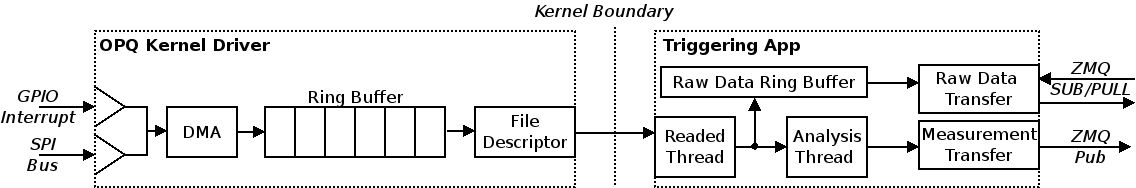
\includegraphics[width=0.9\textwidth]{img/opqbox_software.png}
  \end{center}
  \caption{Block diagram of the OPQ Box 2 software stack.}
  \label{fig:opq:3}
\end{figure}

Raspberry Pi SBC is responsible for signal analysis and anomaly detection.
The Raspberry Pi model used in OPQ Box is the Pi Zero W equipped with 256MB of main memory and a single core 1GHz ARM11 CPU. Furthermore, Pi Zero W is equipped with an on-board 802.11n WIFI transceiver, which removes the need for an external WIFI dongle used in previous OPQ Box devices.
\subsection{Software}\label{subsec:software}
The software stack of the Raspberry Pi aims to deliver a full featured power quality analysis framework despite its rather limited hardware capabilities.
A block diagram of the software stack is shown in Figure~\ref{fig:opq:3}.
Digital data is transferred from the DSP to the Raspberry Pi via Serial Peripheral Interface, with the Pi acting as the master and the DSP as a slave device.
A hardware interrupt line is used to inform Pi software that the DSP is ready for the data transfer.
During the initial design of the OPQ Box 2 software, SPI data transfer was attempted in userland.
However due to the lack of support for DMA in the SPI kernel-to-userland bridge, a large portion of the CPU time was spent facilitating data transfer, resulting in degraded analysis performance as well as missed data samples.
Current revision of the OPQ Box 2 software stack utilizes a kernel driver for management of SPI bus.
Internally OPQ driver maintains a ring buffer of 16 windows each 200 data samples in size.
Upon the receiving the interrupt for the DSP, the CPU sets up the DMA transfer and the DMA engine transfers a 200 sample window into the kernel memory without CPU interaction.
This scheme requires the CPU to only service 60 interrupts a second, with each interrupt requiring on the order of 100 instructions, yielding the CPU utilization of less then $1\%$ in normal operation.
Userland applications communicate with the kernel driver using a file descriptor, where every $write$ system call yields 200 samples of raw waveform.
Thus the smallest window that a userland application may process is a single AC cycle of the grid mains.

Userland component of the OPQ Box 2 software is a multi-threaded extensible analysis framework called Triggering.
The reader thread is responsible for transferring and accumulating data from the kernel driver.
The smallest data buffer that the Triggering application processes at any given time is 10 grid cycles or 2k samples.
Once the cycles are transferred to the userland and timestamped, they are passed to the analysis thread for feature extraction, as well as to the Raw Data Ring Buffer (RDRB).
Since internally all data is addressed using shared pointers, during data duplication no copying is required.
RDRS is capable of buffering up to an hour of historic data before it's overwritten resulting in the RDBS maximum size of 100MB.

Analysis thread of the Triggering application performs feature extraction of the raw data windows of 2000 samples.
Four metrics are extracted from the data stream:
\begin{itemize}
	\item Fundamental frequency.
	\item RMS Voltage.
	\item Total Harmonic Distortion.
	\item Transient.
\end{itemize}

\subsection{Fundamental Frequency}\label{subsec:fundamental-frequency}

Fundamental frequency is calculated by computing the zero crossings of the AC waveform.
Since a sinusoid has two zero crossings for a full cycle the frequency can be calculated as:
\begin{equation} \label{eq:1}
 f = \frac{1}{\frac{2}{n}\sum\limits_{k=0}^{k=n}{\Delta t_{k}}}
\end{equation}

\begin{figure}[h]
	\centering
	\begin{subfigure}{.5\textwidth}
	  \centering
	  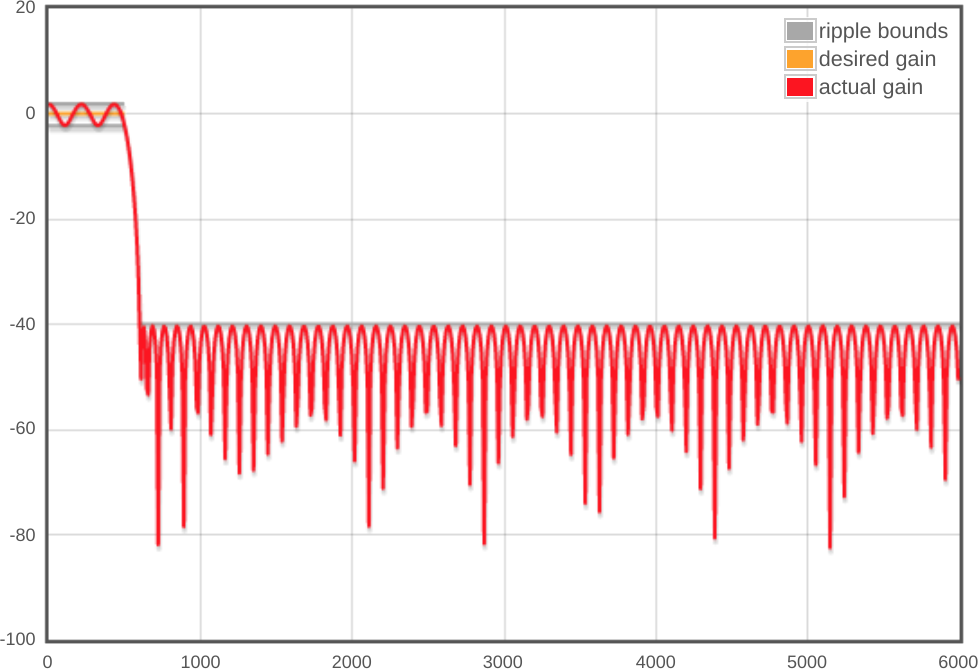
\includegraphics[width=0.9\linewidth]{img/filter1_gain.png}
	  \caption{}
	  \label{fig:opq:4:1}
	\end{subfigure}%
	\begin{subfigure}{.5\textwidth}
	  \centering
	  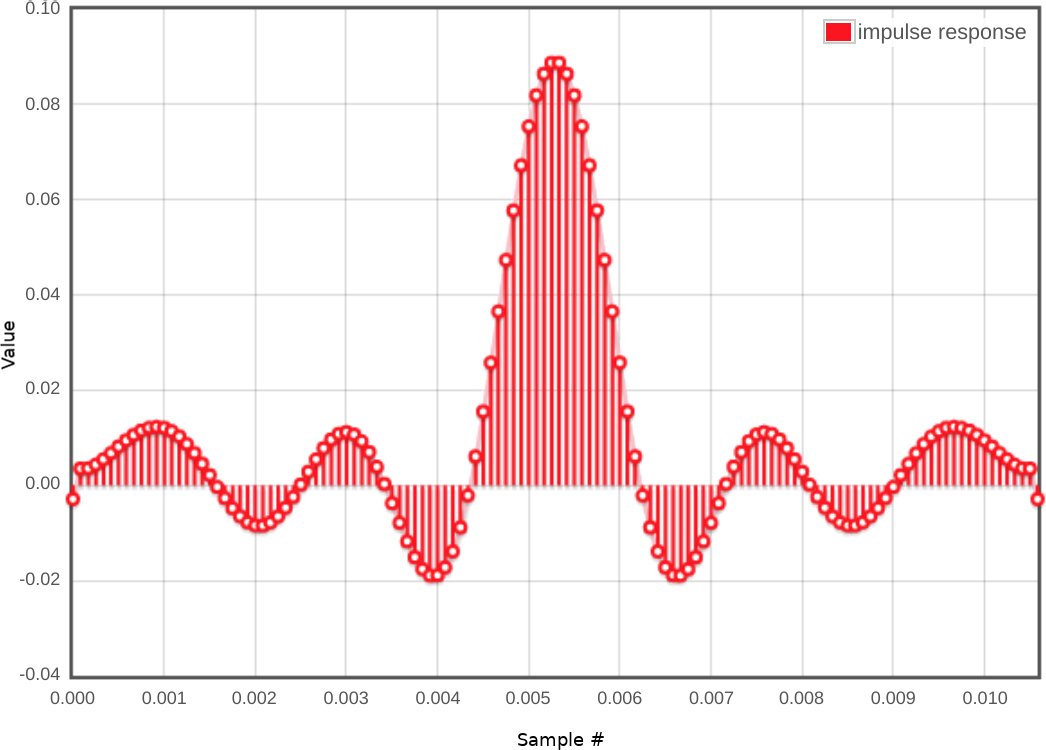
\includegraphics[width=0.9\linewidth]{img/filter1_response.png}
	  \caption{}
	  \label{fig:opq:4:2}
	\end{subfigure}

	\begin{subfigure}{.5\textwidth}
	  \centering
	  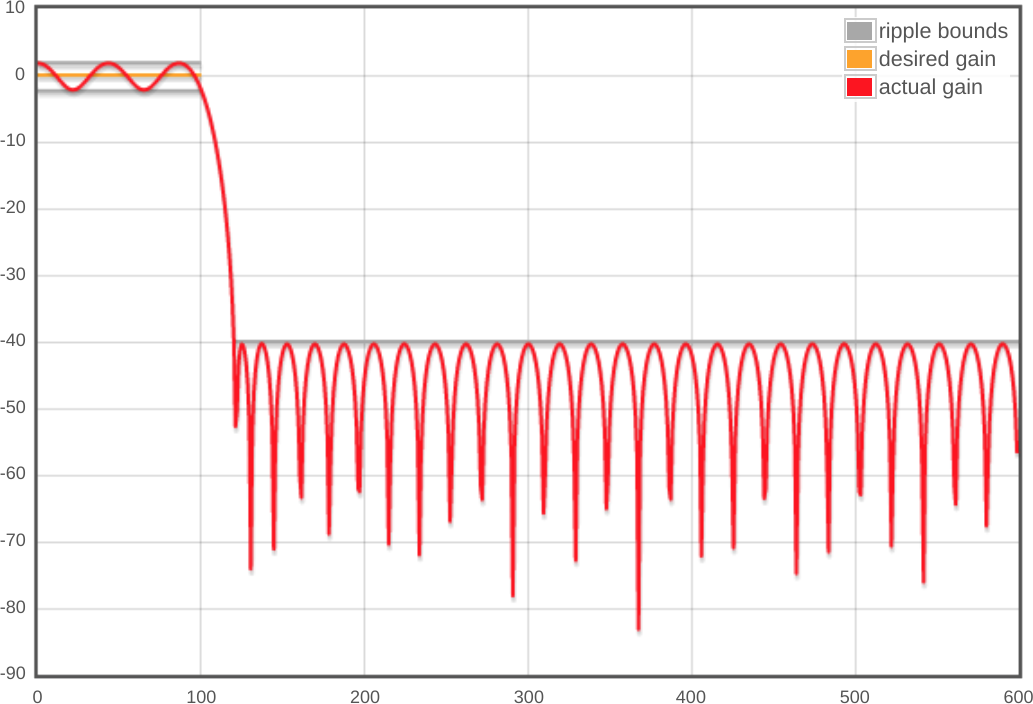
\includegraphics[width=0.9\linewidth]{img/filter2_gain.png}
	  \caption{}
	  \label{fig:opq:4:3}
	\end{subfigure}%
	\begin{subfigure}{.5\textwidth}
	  \centering
	  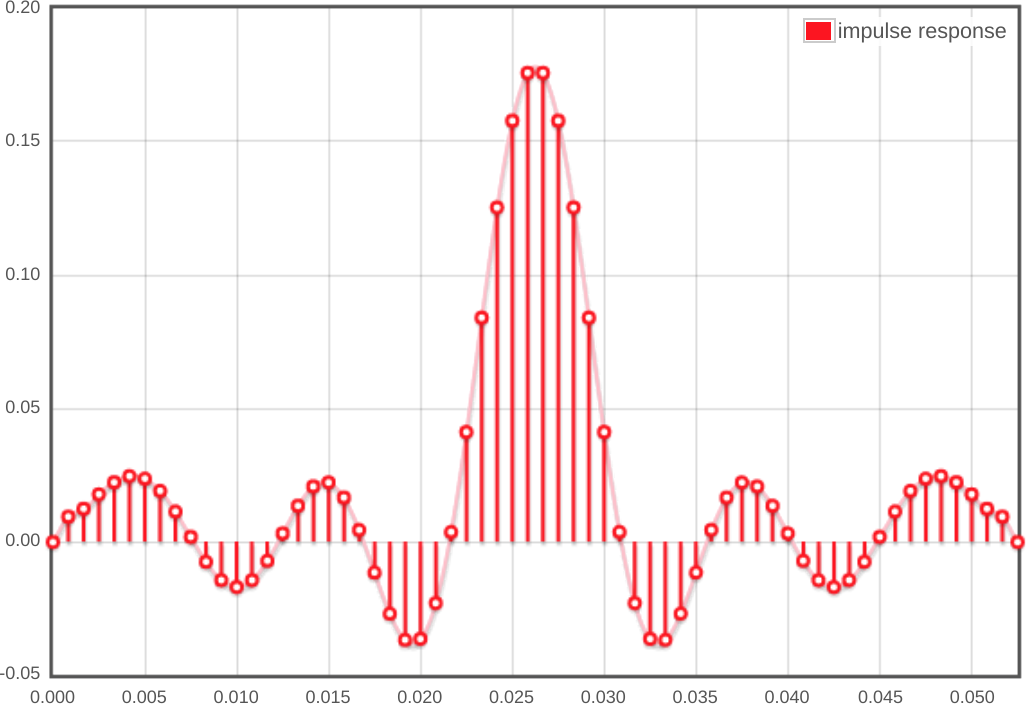
\includegraphics[width=0.9\linewidth]{img/filter2_response.png}
	  \caption{}
	  \label{fig:opq:4:4}
	\end{subfigure}
	\caption{Filters used for mains frequency calculation. (a) Downsampling filter gain. (b) Downsampling filter impulse response. (c) Lowpass filter gain. (d) Lowpass filter impulse response.}
	\label{fig:opq:4}
\end{figure}

Where the $\Delta t_{k}$ is the k'th time between two adjacent zero crossings.
In order to improve the accuracy of the frequency calculation one must first filter out as much noise as possible.
Since our sampling rate is quite high (12kSps) and the fundamental frequency is quite low (60Hz) it is very computationally expensive to perform this filtering in a single step.
Instead filtering is accomplished via a set of two finite impulse response (FIR) filters shown in Figure~\ref{fig:opq:4:2} and~\ref{fig:opq:4:4}.
First the Down sampling filter is applied to the raw waveform, which results in the frequency response shown in Figure~\ref{fig:opq:4:1}.
As is evident by the plot the frequency content of the result is 0-600Hz, Thus it can be downsampled to the $\frac{N}{10}$, or 200 samples without aliasing.
Next the low pass filter is applied to the downsampled waveform with the frequency response shown in Figure~\ref{fig:opq:4:3}.This resulting frequency content is 0-100Hz, thus all of the higher frequency harmonics and noise are removed.
Finally the twice filtered downsampled waveform is used to estimate the fundamental frequency according to the Equation~\ref{eq:1}.
The zero crossings themselves were calculated by using linear interpolation between two points which bracket the time axis.

All electrical generation systems connected to the grid run synchronously with each other, meaning that while small variations in voltage are common across locations, the fundamental frequency and phase must remain strictly in sync.
This effect is demonstrated in Figure~\ref{fig:opq:5}, which is a frequency fluctuation event recorded on November 8 2017.
While the two devices were separated by ten miles, their frequency measurements track closely together.

\begin{figure}[h]
	\centering
	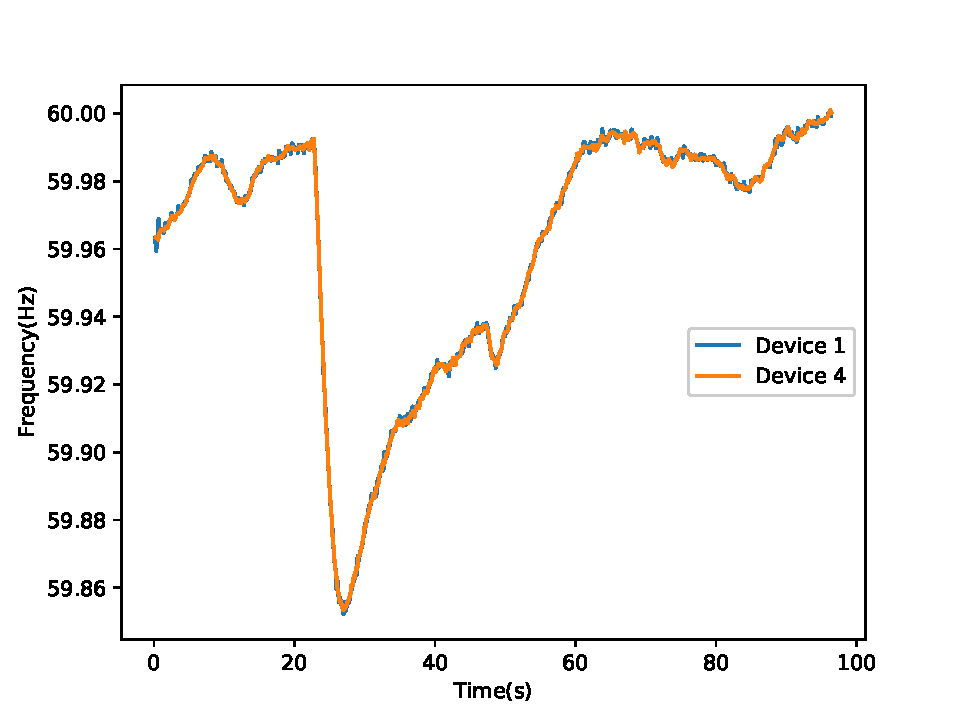
\includegraphics[width=0.6\linewidth]{img/frequency_two_devices.pdf}
	\caption{Frequency measurement across two devices recorded during a lighting strike.}
	\label{fig:opq:5}
\end{figure}

\subsection{Root Mean Square Voltage}\label{subsec:root-mean-square-voltage}

Root mean square voltage ($V_{rms}$) in electrical power is the equivalent value of DC voltage which would dissipate the same power in the resistive load. $V_{rms}$ is a convenient measure for detecting voltage sags and swells, since they result in nominally higher and lower computed value.
For the sinusoidal signal $V_{rms}$ can be calculated from the peak to peak value ($V_{pp}$) as:
\begin{equation} \label{eq:2}
	V_{rms} = \frac{V_{pp}}{2\sqrt{2}}
\end{equation}
It is common for multimeter to employ the equation above for computing $V_{rms}$.
However this equation is only valid for a perfect sinusoid, and thus does not result in a suitable metric for identifying power quality disturbances.
Instead OPQ Box 2 computes $V_{rms}$ as follows:
\begin{equation} \label{eq:3}
	V_{rms} = \sqrt{\frac{1}{n}\sum\limits_{k=0}^{k=n}V_{k}^{2}}
\end{equation}
Similarly to the frequency calculation OPQ Box 2 usees a 10 cycle window for a single $V_{rms}$ calculation, however unlike the frequency calculation the input is not filtered a priori.
An example of a power quality disturbance which exhibits low $V_{rms}$ is shown in Figure~\ref{fig:opq:6:1} and~\ref{fig:opq:6:2}.
These disturbances are the result of a lighting strike recorded by two OPQ Box 2 devices on Nov 1, 2017.

\begin{figure}[h]
		\centering
	\begin{subfigure}{.5\textwidth}
	  \centering
	  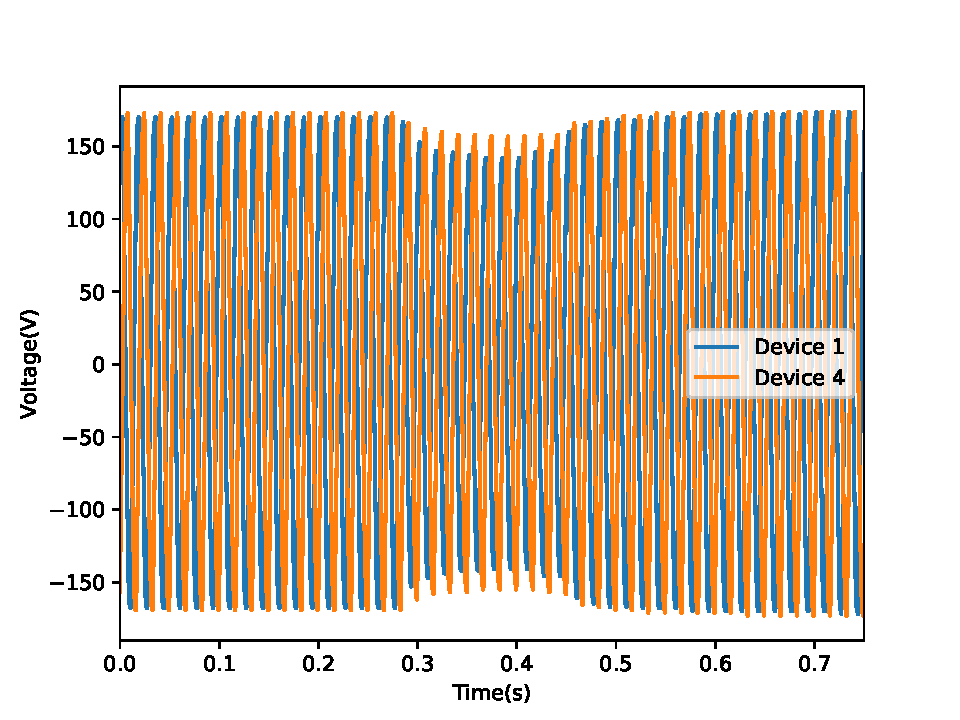
\includegraphics[width=0.9\linewidth]{img/voltage_sag.pdf}
	  \caption{}
	  \label{fig:opq:6:1}
	\end{subfigure}%
	\begin{subfigure}{.5\textwidth}
	  \centering
	  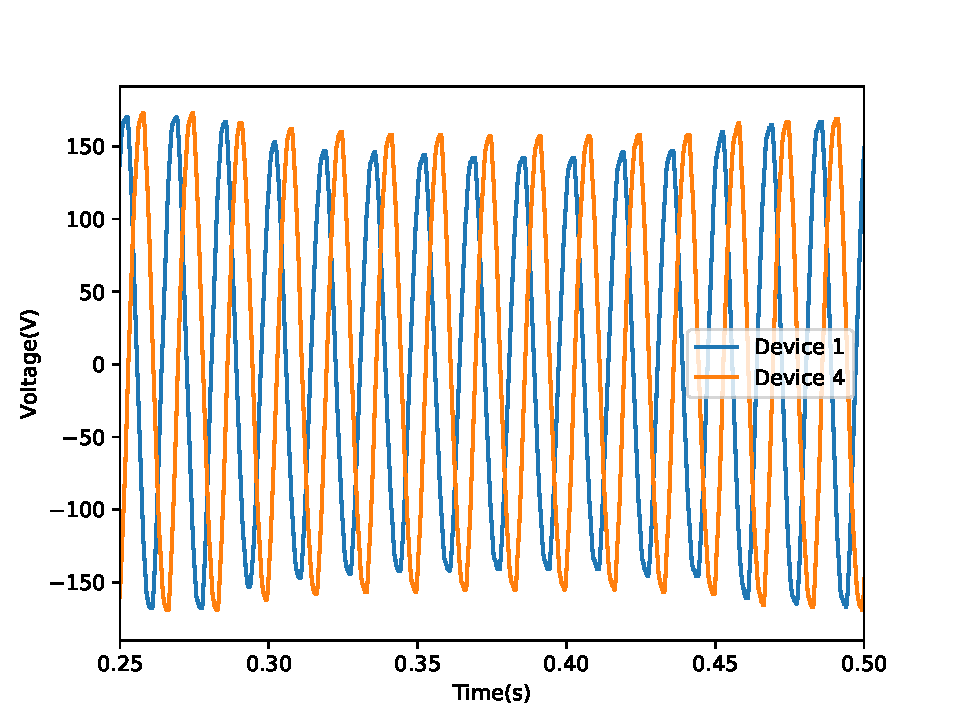
\includegraphics[width=0.9\linewidth]{img/voltage_sag_zoomed_in.pdf}
	  \caption{}
	  \label{fig:opq:6:2}
	\end{subfigure}
	\caption{A lightning strike recorded by two OPQ Box 2 devices separated by 10 miles. (a) A lightning strike manifested as $V_{rms}$ dip which lasted 11 cycles. (b) As a consequence of using NTP these devices have $\frac{1}{2}$ cycle mismatch in reported timestamps.}
	\label{fig:opq:6}
\end{figure}


\subsection{Total Harmonic Distortion}\label{subsec:thd}
OPQ Box calculates THD using industry standard methodology.
In the power delivery industry THD is defined as:
\begin{equation} \label{eq:4}
THD = \frac{\sqrt{\sum{V_{n}^2}}}{V_{f}}*100\%
\end{equation}
Where $V_{f}$ is the fundamental 60Hz power and $V_{n}$ is the power at $n^{th}$ harmonic.
It should be noted that in the power quality domain THD is expressed as a percentage as opposed to $\frac{dB}{\sqrt{Hz}}$ as used in other disciplines.
Operationally, OPQ Box computes THD for 10 cycles of the fundamental frequency.
First an FFT transforms the real voltage samples into it's frequency components.
Next, the square of the harmonic bins is accumulated and scaled by the magnitude of the fundamental power.

\begin{figure}[h]
	\centering
	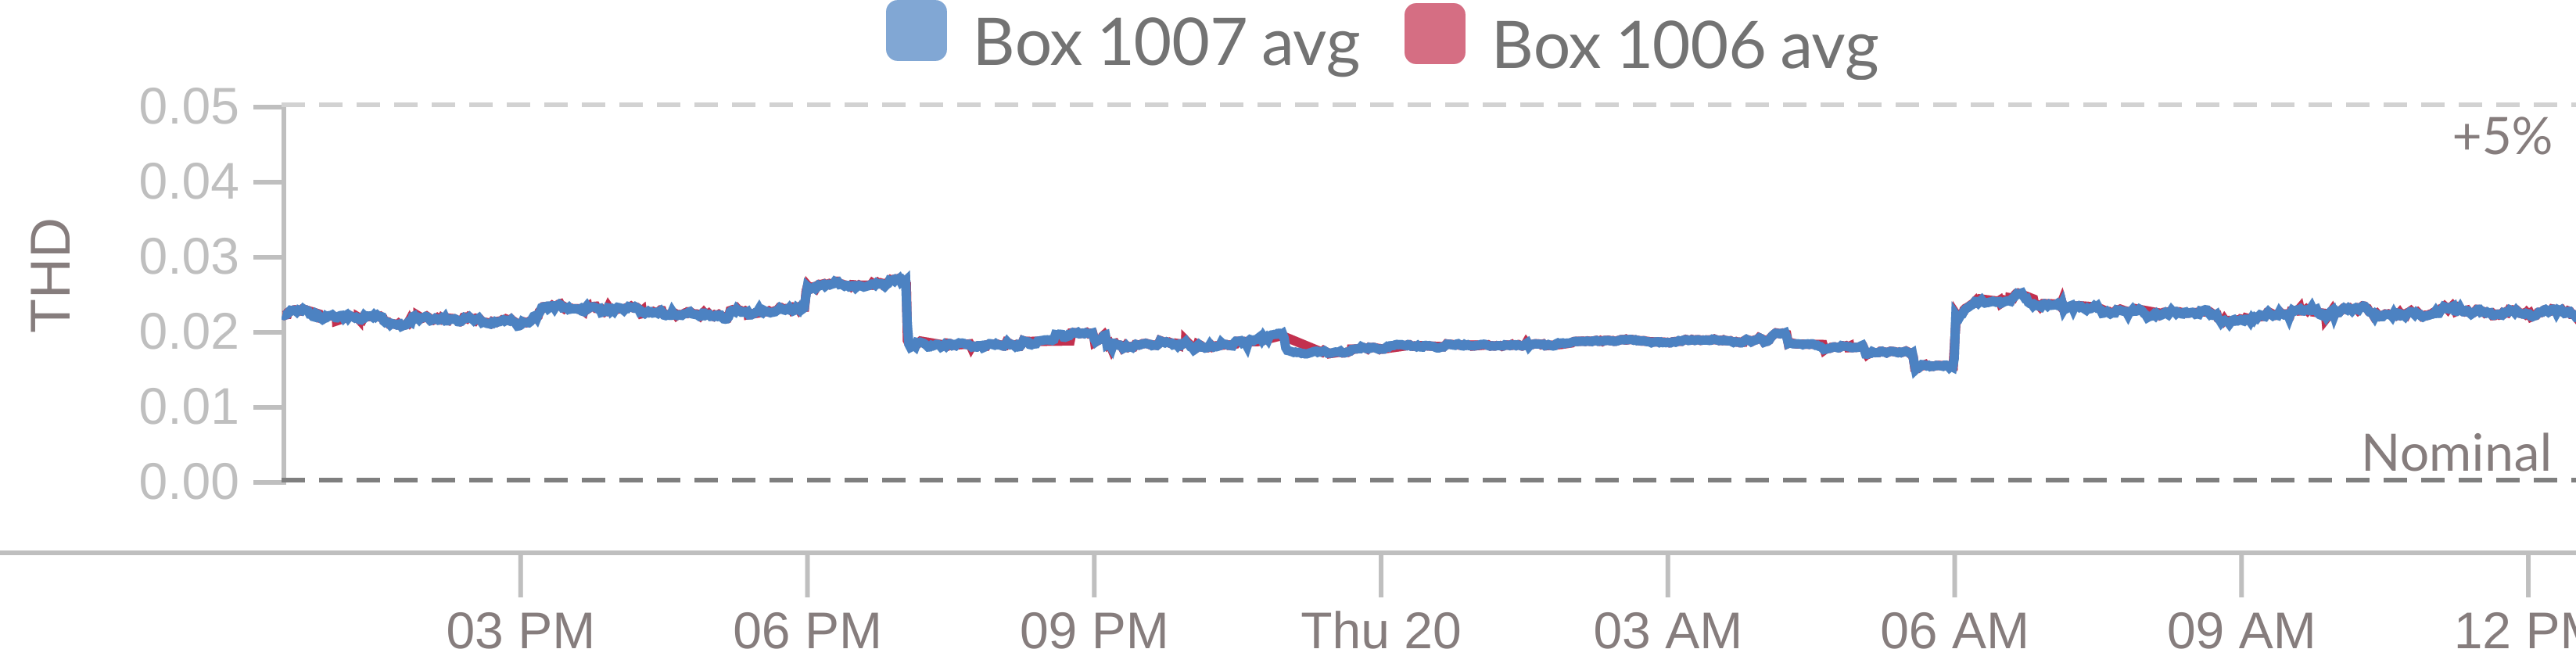
\includegraphics[width=1\linewidth]{img/thd_two_devices_24_hours.png}
	\caption{A common THD trend across two OPQ Box devices each deployed in the two Flexible Response to Ongoing Growth buildings on UH campus.}
	\label{fig:opq:7}
\end{figure}

Figure~\ref{fig:opq:7} shows a common trend observed by all OPQ Box devices installed on the UH campus.
For clarity only two devices are shown.
It is assumed that the large drop observed daily from approximately 6am to 6pm corresponds to the automatic response of the power delivery system to the reactive power in the grid, by deploying a large capacitor bank to compensate for the current phase lag.

\subsection{Transient Detection}\label{subsec:transient-detection}

OPQ Box transient detection is performed via filtering out of the fundamental frequency via an FIR high pass pass filter and searching for a maximum value in the remainder.
The high pass filter has a cutoff of $400Hz$, and the filter coefficients and response are shown in Figure~\ref{fig:opq:8:2} and Figure~\ref{fig:opq:8:1} respectively.
The result of the high pass filter operation is shown in Figure~\ref{fig:opq:8}.
Figure~\ref{fig:opq:8:3} shows a synthetic signal generated via a SDG1025 signal generator and fed into the OPQ Box.
This signal contains a $5V_{pp}$ transient injected at 11ms.
Filtered signal is shown in Figure~\ref{fig:opq:8:4}, with the fundamental removed and the transient preserved.
OPQ Box scans for the highest sample in the filtered waveform and uses its magnitude as a transient detection metric.


\begin{figure}[h]
	\centering
	\begin{subfigure}{.5\textwidth}
		\centering
		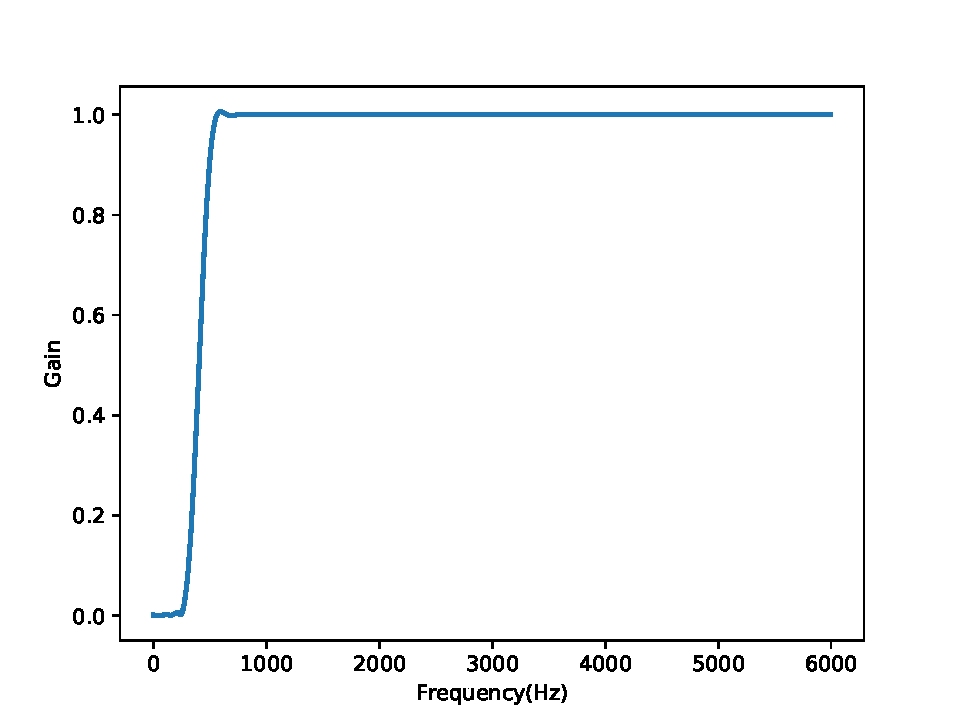
\includegraphics[width=1\linewidth]{img/thd_hpf_resp.pdf}
		\caption{}
		\label{fig:opq:8:1}
	\end{subfigure}%
	\begin{subfigure}{.5\textwidth}
		\centering
		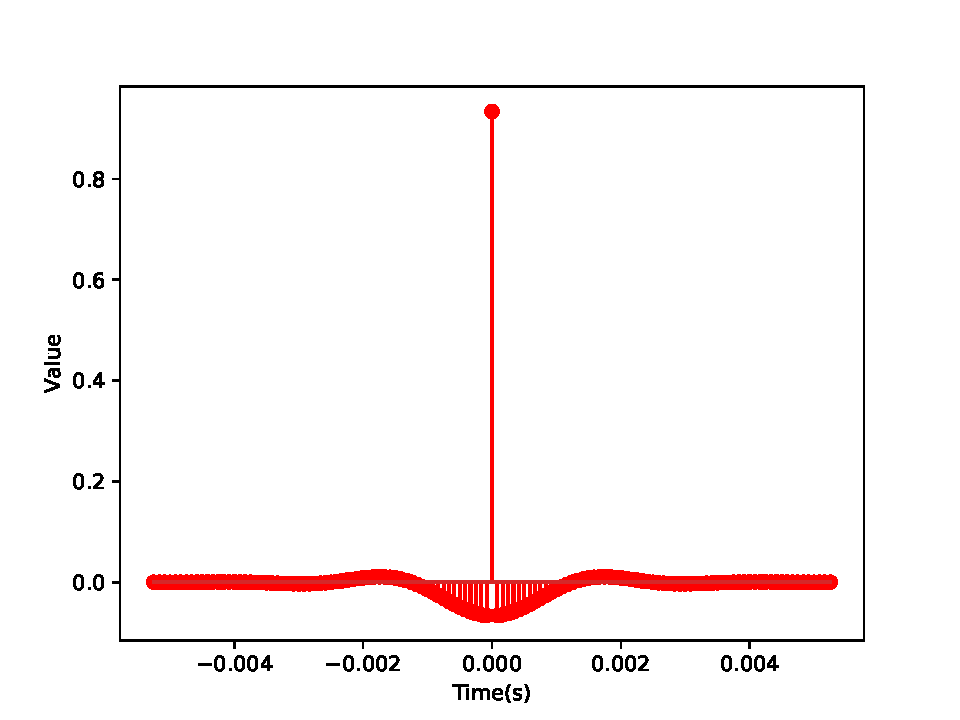
\includegraphics[width=1\linewidth]{img/thd_hpf.pdf}
		\caption{}
		\label{fig:opq:8:2}
	\end{subfigure}

	\begin{subfigure}{.5\textwidth}
		\centering
		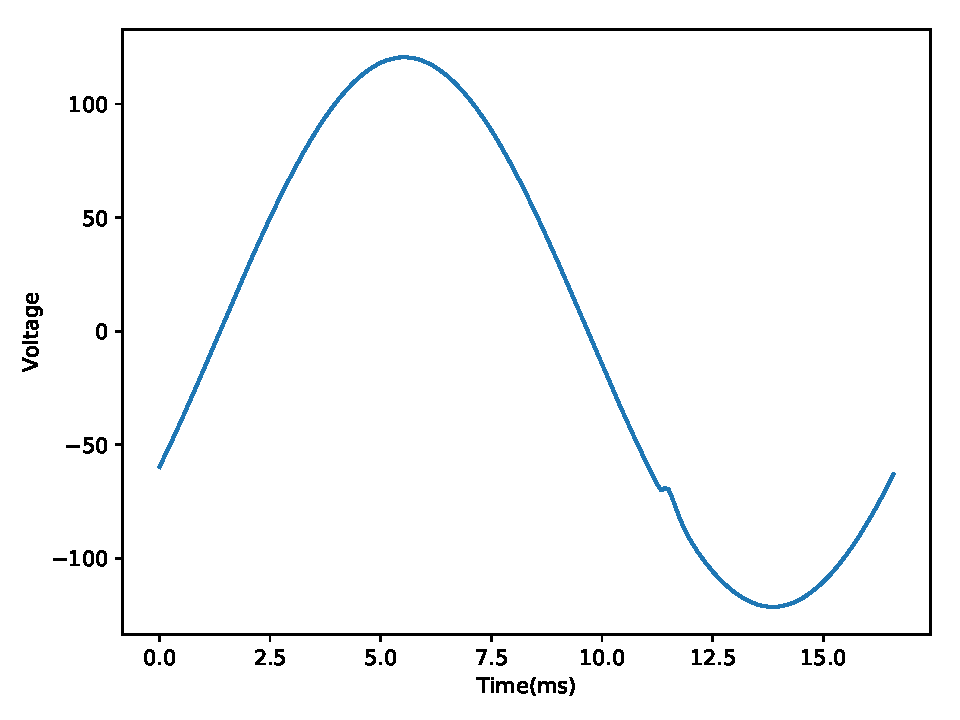
\includegraphics[width=0.86\linewidth]{img/box_eval/5v_transient.pdf}
		\caption{}
		\label{fig:opq:8:3}
	\end{subfigure}%
	\begin{subfigure}{.5\textwidth}
		\centering
		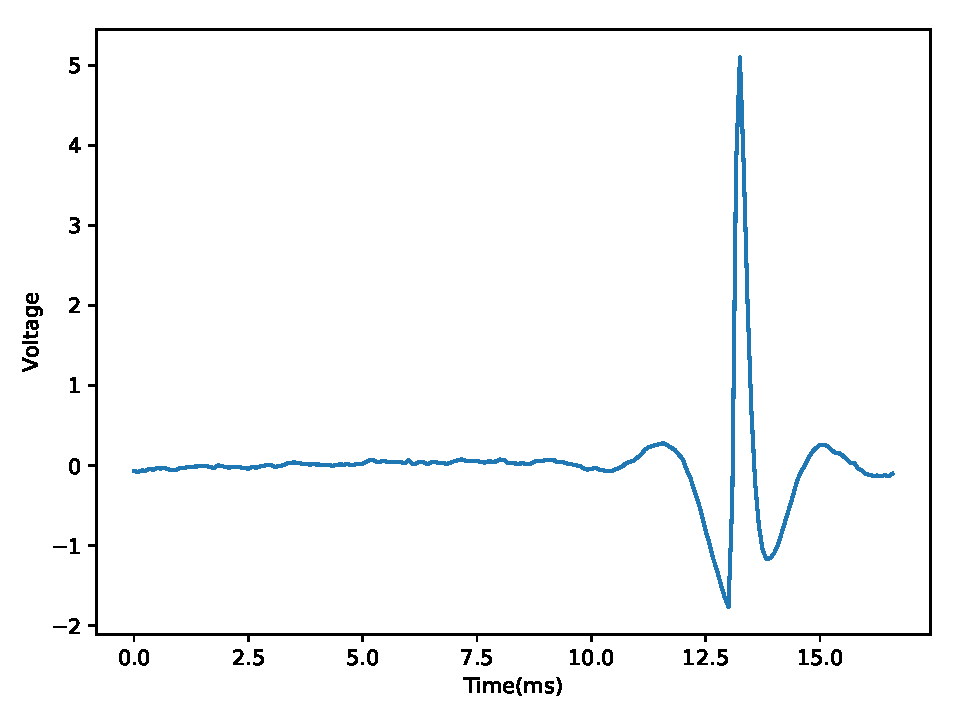
\includegraphics[width=0.86\linewidth]{img/box_eval/5v_transient_filtered.pdf}
		\caption{}
		\label{fig:opq:8:4}
	\end{subfigure}
	\caption{THD detection filtering. (a) Filter gain. (b) Filter response. (c) A 5V transient superimposed onto a fundamental. (d) Filter result from (c).}
	\label{fig:opq:8}
\end{figure}

It should be noted, that this transient detection method is susceptible to THD fluctuations, since any harmonic above $400Hz$ will remain in the filtered waveform.
However, since the THD information is transmitted along with the transient detection metric, they can be correlated in downstream transient detection.
This effect can be seen in Figure~\ref{fig:opq:9}.
This figure shows both the THD and transient detection metric during a transient event.
A small transient of approximately 1.6V was observed occurring at 2600s, while the sensitivity of the transient metric is clearly visible, particularly between 3000s and 4500s.

\begin{figure}[h]
	\begin{center}
		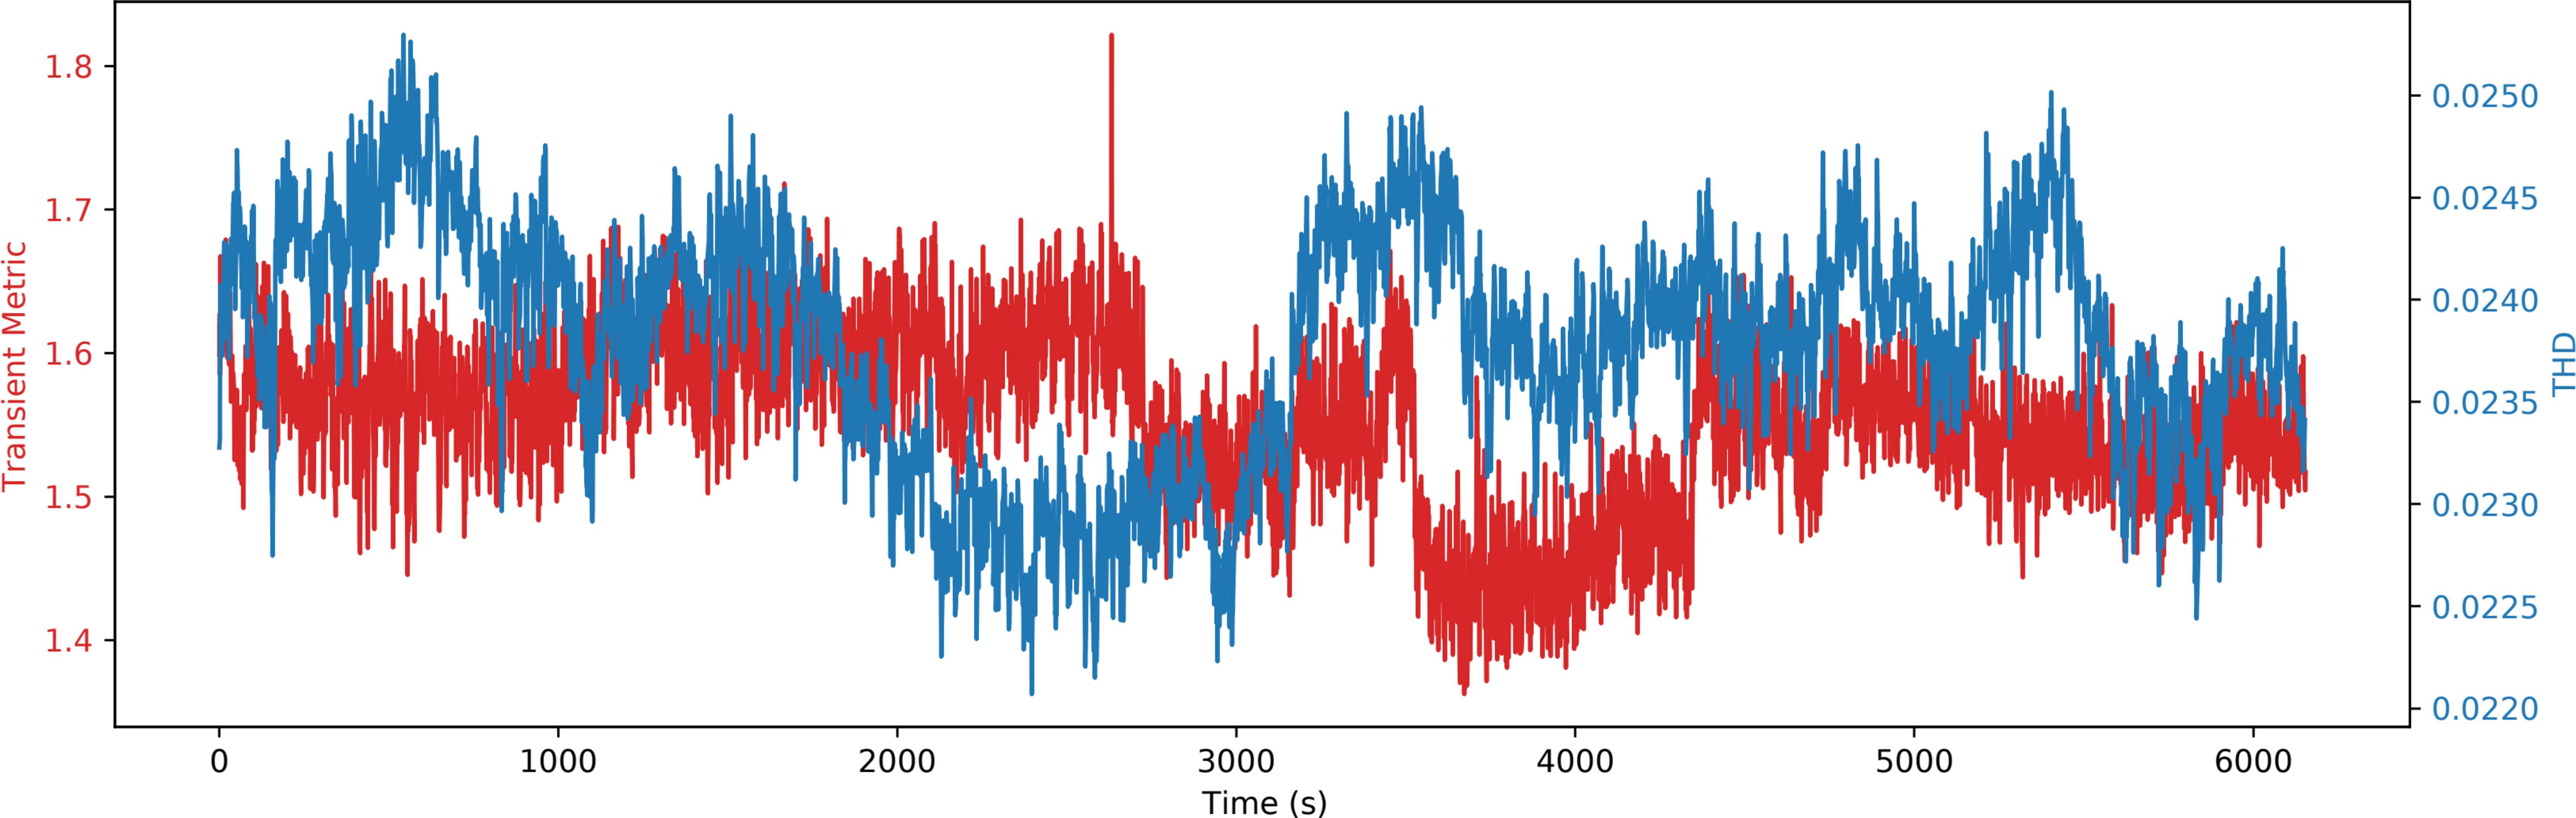
\includegraphics[width=1\textwidth]{img/trans_thd_det.pdf}
	\end{center}
	\caption{THD and Transient detection metric.}
	\label{fig:opq:9}
\end{figure}

\subsection{Network Communication}\label{subsec:network-communication}

Computed fundamental frequency and $V_{rms}$ are transmitted to the Makai service for aggregation.
Data transmission is handled using 0MQ software stack with Curve25519 elliptic curve encryption.
Each device holds a unique private and public key, as well as the servers public key, allowing both the Makai service and the OPQ Box 2 to verify it's peer.
Internally metrics transmission uses 0MQ's PUB/SUB protocol.
This protocol is a publish subscribe topology, with each message containing the topic, and a payload.
Additionally 0MQ pub-sub topology allows for multiple sub peers with subscriptions forwarder to the publisher automatically via a side channel.
This allows for the aggregation service to be spread across multiple nodes, with minimal network overhead.

If the aggregation service determines that an anomaly has occurred, it is able to request raw waveform from the OPQ Box 2 RDRB via a separate 0MQ pub sub channel.
If the RDRB buffer contains data for the requested temporal range, OPQ Box 2 transmits the available data to the aggregation service via a push pull 0MQ channel.
Protobuf message serialization is used to encode messages across the OPQ ecosystem.


In order to make a distributed measurement, all of the OPQ Boxes on the OPQ network need to maintain an accurate time reference.
Time synchronization across multiple OPQ Boxes is accomplished using the Network Time Protocol.
The expansion port of the OPQ Box 2 supports a GPS receiver.
GPS receivers require line of sight to the sky, and since the with out on-board real-time clock, every power interruption requires a GPS cold start.
NTP performance has been verified against GPS resulting in time error of $8ms\pm 5ms$ which is typical for NTP running over the Internet with a close by NTP server.
This error is visualized in a Figure~\ref{fig:opq:6:2}.
With a large coincidental $V_{pp}$ drop across two devices, a 7ms phase error is clearly visible.


\section{OPQ Makai}\label{sec:opq-makai}

OPQ Makai implements the Napali Framework requirements for a ``sink''.
 It is a distributed extensible microservice framework responsible for receiving the triggering stream from the OPQ Boxes, locating anomalous temporal regions and requesting raw waveform for the anomalous time ranges.
 As evident from the block diagram shown in Figure~\ref{fig:opq:10}, Makai consists of four major components: Acquisition Broker, Triggering Broker, Event Service and the Acquisition Service.
\begin{figure}[h]
  \begin{center}
  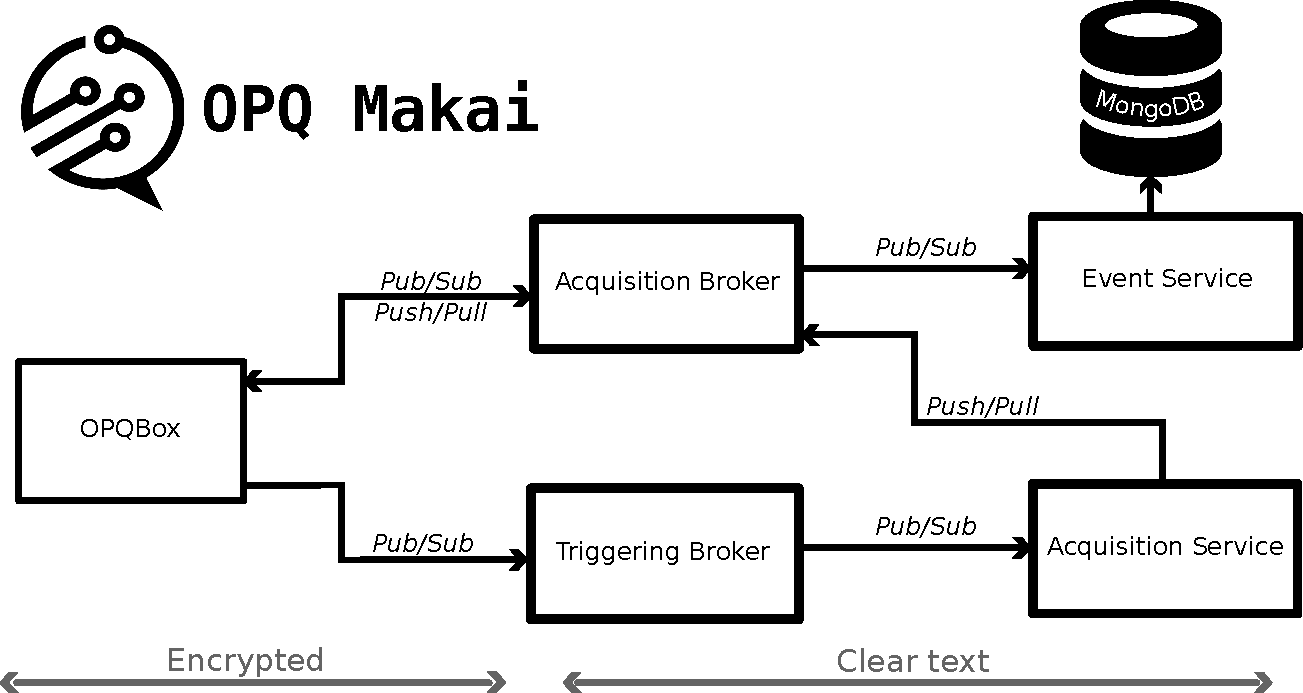
\includegraphics[width=0.7\textwidth]{img/makai_main.pdf}
  \end{center}
  \caption{Block diagram of the OPQ Makai.}
  \label{fig:opq:10}
\end{figure}

\subsection{Triggering Broker}\label{subsec:triggering-broker}

The triggering Broker is perhaps the simplest component of the OPQ Makai system.
The triggering stream generated by the OPQ Boxes is encrypted to preserve users privacy.
In order to minimize the CPU time spent decrypting the data across multiple OPQ services, the Triggering Broker is used to decrypt the data and send clear text measurements across the rest of the OPQ ecosystem.
Triggering Broker uses the 0mq subscribe socket to receive data form OPQ Boxes, and sends it via a publish socket to any connected client.
Each publish message is published to a topic which corresponds to the ASCII representation of the originating OPQ Box ID.
This allows services which utilize the Triggering broker to select a subset of IDs to operate on.
This is useful for load balancing the backend services, or dividing the OPQ network into separate regions with no electrical connections between them.

OPQ Box transmits metrics which make up the triggering stream in form of protobuf encoded messages.
The structure of triggering messages is shown in Table \ref{tbl:opq:trg_struct}.
\begin{center}
	\begin{table}[!ht]
		\caption{Triggering message structure.}
		\label{tbl:opq:trg_struct}
		\begin{tabularx}{\textwidth}[t]{ssb}
			\arrayrulecolor{green}\hline
			\textbf{\textcolor{myGreen}{Triggering Message}} & &\\
			\hline
			\textbf{Field} & \textbf{Type} & \textbf{Description} \\
			\arrayrulecolor{black}\hline
			\textbf{box\_id} & \textit{uint32} & Device ID this message originated from.\\
			\arrayrulecolor{black}\hline
			\textbf{timestamp\_ms} & \textit{uint64} & Timestamp corresponding to the first cycle in the temporal window.\\
			\arrayrulecolor{black}\hline
			\textbf{metrics} & \textit{map$<$string, Metric$>$} & A map of metric names to corresponding values.\\
			& & \\
			\arrayrulecolor{green}\hline
			\textbf{\textcolor{myGreen}{Metric}} & &\\
			\hline
			\textbf{Field} & \textbf{Type} & \textbf{Description} \\
			\arrayrulecolor{black}\hline
			\textbf{min} & \textit{f32} & Minimum observed in this window.\\
			\arrayrulecolor{black}\hline
			\textbf{max} & \textit{f32} & Maximum observed in this window.\\
			\arrayrulecolor{black}\hline
			\textbf{average} & \textit{f32} & Average observed in this window.\\
		\end{tabularx}
	\end{table}
\end{center}


\subsection{Acquisition Broker}\label{subsec:acquisition-broker}

The Acquisiton Broker manages the two way communication between the OPQ Boxes and the rest of the cloud infrastructure.
Unlike the triggering stream which originates from the OPQ Box, two way communication is always initiated by the cloud services.
Two way communication is realized via a command response interface, where the OPQ service initiates the communication by sending in clear text command to the Acquisition Broker, which then forwards it in the encrypted form to the appropriate OPQ Boxes.

As mention in the OPQ Box section, all communication between the OPQ Box and Makai is serialized using Google protobuf.
Protobuf allows for polylingual communication between software components across network boundaries.
This is particularly important in case of the Acquisition and Triggering brokers, since they facilitate all inter-network communication.
All commands between services downstream of the Acquisition Broker and OPQ Boxes take on the form shown in Table \ref{tbl:opq:cmd_struct}.

\begin{center}
	\begin{table}[!ht]
		\caption{Command/Response message structure.}
		\label{tbl:opq:cmd_struct}
		\begin{tabularx}{\textwidth}[t]{ssb}

			\arrayrulecolor{green}\hline
			\textbf{\textcolor{myGreen}{Makai $\rightarrow$ OPQ Box}} & &\\
			\hline
			\textbf{Field} & \textbf{Type} & \textbf{Description} \\
			\arrayrulecolor{black}\hline
			\textbf{seq} & \textit{uint32} & Sequence number for the command.\\
			\arrayrulecolor{black}\hline
			\textbf{box\_id} & \textit{uint32} & Device ID this command will be routed to.\\
			\arrayrulecolor{black}\hline
			\textbf{timestamp\_ms} & \textit{uint64} & Millisecond timestamp, created on command issue.\\
			\arrayrulecolor{black}\hline
			\textbf{identity} & \textit{string} & Identity of the sender.\\
			\arrayrulecolor{black}\hline
			\textbf{command} & \textit{Command} & Command payload.\\
			& &\\
			\arrayrulecolor{green}\hline
			\textbf{\textcolor{myGreen}{OPB Box $\rightarrow$ Makai}} & &\\
			\hline
			\textbf{Field} & \textbf{Type} & \textbf{Description} \\
			\arrayrulecolor{black}\hline
			\textbf{box\_id}  & \textit{uint32} & Device ID this command is routed from.\\
			\arrayrulecolor{black}\hline
			\textbf{seq} & \textit{uint32} & Sequence number of the response\\
			\arrayrulecolor{black}\hline
			\textbf{timestamp\_ms} & \textit{uint64} & Millisecond timestamp, created on response issue.\\
			\arrayrulecolor{black}\hline
			\textbf{response} & \textit{Response} & Response payload.\\
		\end{tabularx}
	\end{table}
\end{center}

In order to send a message to an OPQ Box client generates a \textbf{Makai $\rightarrow$ OPQ Box} command containing its identity, serializes it, and forwards it to the Acquisition brokers push port.
Acquisition broker assigns a unique sequence number to the request and stores a it in an internal synchronized key value store along with the sender identity.
The message is re-serialized and sent out to the desired OPQ Box via the brokers encrypted pub interface.
Each message sent to the OPQ Box generates a response in form of \textbf{OPB Box $\rightarrow$ Makai} message.
This response is received by the Acquisition broker via encrypted pull interface, deserialized and validated.
Response sequence number is used to determine the recipients identity, and the message is forwarded to the correct recipient via brokers cleartext publish interface.
It is important to note that the service which generates a command and a service which receives the response need not be the same, and a command originator may place the box response into the subscribe stream of a different service.
This detail will becomes important during the discussion of the Event service.
Furthermore, sending and receiving messages occurs asynchronously, thus multiple clients can communicate with multiple Boxes at the same time.
Finally a garbage collector cleans the synchronised key value store every hour, removing sequence numbers which did not receive a response for an OPQ Box.
These sequence numbers and identities are logged, since a lack of a response indicates a device or a network fault, or a buggy client.

There are four unique payload commands/responses which an OPQ Box understands.
These payloads are ignored by the Acquisition Broker and are simply forwarded to the recipient.
Bellow is the list of commands/responses:
\begin{itemize}
	\item{\textbf{(HEALTH) Health:}} The health command is broadcast periodically across all of the OPQ Boxes, in order to monitor the health of the OPQ network.
	The OPQ Box response to this command contains diagnostic information, such as the timestamp of the last event requested, ip address and the name and strength of the WIFI network the OPQ Box is connected to.
	\item{\textbf{(CMW) Change measurement window:}} This command allows to vary how often a triggering stream message is generated and delivered to the triggering broker.
	This is accomplished by varying the length of the temporal window used to derive the triggering metrics.
	\item{\textbf{(RD) Send raw data:}} This command instructs the OPQ Box to send data from the its raw data buffer to the cloud.
	\item {\textbf{(PLG) Plugin:}} Send a binary payload directly to a OPQ Box Plugin.
\end{itemize}
Data fields for each command are described in the Tables \ref{tbl:opq:cmd_payload} and \ref{tbl:opq:rsp_payload}.
Notice that an \textbf{Err} response does not correspond to any commands described above.
OPQBox generates this response under following conditions:
\begin{itemize}
	\item Command payload could not be parsed.
	\item $start\_ms > end\_ms$ in case of the RD command.
	\item box\_id field does not match the destination OPQ Box.
	\item PLG command is attempting to route to a OPQ Box plugin that is not loaded by the recipient.
\end{itemize}
In the current implementation OPQ Makai protocol does not support multicast addressing of OPQ Boxes.
Furthermore, due to the limitations of the 0MQ API, there is no stable method of querying the clients connected to a particular port.
Utilities which query all available devices, such as a periodic health check service, query the Mongo database for a list of devices registered to the OPQ network, and send their queries to each box individually.
\begin{center}
	\begin{table}[!ht]
		\caption{Command Payloads}
		\label{tbl:opq:cmd_payload}
		\begin{tabularx}{\textwidth}[t]{ssb}

			\arrayrulecolor{green}\hline
			\textbf{\textcolor{myGreen}{HEALTH}} & &\\
			\hline
			N/A & & This command has no fields.\\
			& &\\
			\arrayrulecolor{green}\hline
			\textbf{\textcolor{myGreen}{CMW}} & &\\
			\hline
			\textbf{Field} & \textbf{Type} & \textbf{Description} \\
			\arrayrulecolor{black}\hline
			\textbf{measurement\_rate}  & \textit{uint32} & Number of cycles per triggering triggering message.\\
			& &\\
			\arrayrulecolor{green}\hline
			\textbf{\textcolor{myGreen}{RD}} & &\\
			\hline
			\textbf{Field} & \textbf{Type} & \textbf{Description} \\
			\arrayrulecolor{black}\hline
			\textbf{start\_ms} & \textit{uint64} & Timestamp defining the beginning of the region of interest.\\
			\arrayrulecolor{black}\hline
			\textbf{end\_ms} & \textit{uint64} & Timestamp defining the end of the region of interest.\\
			\arrayrulecolor{black}\hline
			\textbf{wait} & \textit{bool} & A flag indicating that a Box must wait if \textbf{end\_ms} is in the future.\\
			& & \\
			\arrayrulecolor{green}\hline
			\textbf{\textcolor{myGreen}{PLG}} & &\\
			\hline
			\textbf{Field} & \textbf{Type} & \textbf{Description} \\
			\arrayrulecolor{black}\hline
			\textbf{plugin\_name} & \textit{string} & Name of the plugin.\\
			\arrayrulecolor{black}\hline
			\textbf{message} & \textit{bytes} & Binary payload for the plugin.\\

		\end{tabularx}
	\end{table}
\end{center}

\begin{center}
	\begin{table}[!ht]
		\caption{Response Payloads}
		\label{tbl:opq:rsp_payload}
		\begin{tabularx}{\textwidth}[t]{ssb}

			\arrayrulecolor{green}\hline
			\textbf{\textcolor{myGreen}{HEALTH}} & &\\
			\hline
			\textbf{Field} & \textbf{Type} & \textbf{Description} \\
			\arrayrulecolor{black}\hline
			\textbf{mac\_addr} & \textit{string} & Mac address of the box.\\
			\arrayrulecolor{black}\hline
			\textbf{wifi\_network} & \textit{string} & SSID of connected Wifi network.\\
			\arrayrulecolor{black}\hline
			\textbf{ip} & \textit{string} & Ip address of the wlan0 interface.\\
			\arrayrulecolor{black}\hline
			\textbf{uptime} & \textit{uint64} & Device uptime in ms.\\
			\arrayrulecolor{black}\hline
			\textbf{calibration\_constant} & \textit{f32} & Calibration constant for the device.\\
			\arrayrulecolor{black}\hline
			\textbf{pub\_key} & \textit{string} & Byte64 encoded public key of the device.\\
			\arrayrulecolor{black}\hline
			\textbf{measurement\_rate} & \textit{string} & How often a triggering message is produced.\\

			& &\\
			\arrayrulecolor{green}\hline
			\textbf{\textcolor{myGreen}{CMW}} & &\\
			\hline
			\textbf{Field} & \textbf{Type} & \textbf{Description} \\
			\arrayrulecolor{black}\hline
			\textbf{measurement\_rate}  & \textit{uint32} & Old measurement rate.\\
			& &\\
			\arrayrulecolor{green}\hline
			\textbf{\textcolor{myGreen}{RD}} & &\\
			\hline
			\textbf{Field} & \textbf{Type} & \textbf{Description} \\
			\arrayrulecolor{black}\hline
			\textbf{start\_ms} & \textit{uint64} & Timestamp defining the beginning of the region of interest.\\
			\arrayrulecolor{black}\hline
			\textbf{end\_ms} & \textit{uint64} & Timestamp defining the end of the region of interest.\\
			\arrayrulecolor{black}\hline
			\textbf{data} & \textit{Cycle[..]} & Data divided into single cycle windows structures. \\
			& & \\
			\arrayrulecolor{green}\hline
			\textbf{\textcolor{myGreen}{Cycle}} & &\\
			\hline
			\textbf{Field} & \textbf{Type} & \textbf{Description} \\
			\arrayrulecolor{black}\hline
			\textbf{datapoints} & \textit{int16[200]} & Raw ADC samples for one cycle window.\\
			\arrayrulecolor{black}\hline
			\textbf{timestamp\_ms} & \textit{uint64} & Timestamp of the last sample.\\
			& & \\
			\arrayrulecolor{green}\hline
			\textbf{\textcolor{myGreen}{PLG}} & &\\
			\hline
			\textbf{Field} & \textbf{Type} & \textbf{Description} \\
			\arrayrulecolor{black}\hline
			\textbf{OK} & \textit{bool} & Flag indicating that the command was successfully routed to a plugin.\\
			& & \\
			\arrayrulecolor{green}\hline
			\textbf{\textcolor{myGreen}{Err}} & &\\
			\hline
			\textbf{Field} & \textbf{Type} & \textbf{Description} \\
			\arrayrulecolor{black}\hline
			\textbf{code} & \textit{uint32} & Error Code.\\
			\arrayrulecolor{black}\hline
			\textbf{Error} & \textit{string} & Human readable error string.\\
		\end{tabularx}
	\end{table}
\end{center}

\subsection{Acquisition Service}\label{subsec:acquisition-service}

The Acquisition Service middleware resides in between the Triggering and Acquisition Brokers.
Acquisition Service is responsible for the following tasks:
\begin{enumerate}
	\item Computation of statistics of the incoming triggering stream.
	\item Hosting plugins for triggering stream analysis.
	\item Generating data event requests for OPQ Boxes.
\end{enumerate}
A block diagram of the Acquisition Service is shown in Figure \ref{fig:opq:makai_aqs}.
\begin{figure}[h]
	\begin{center}
		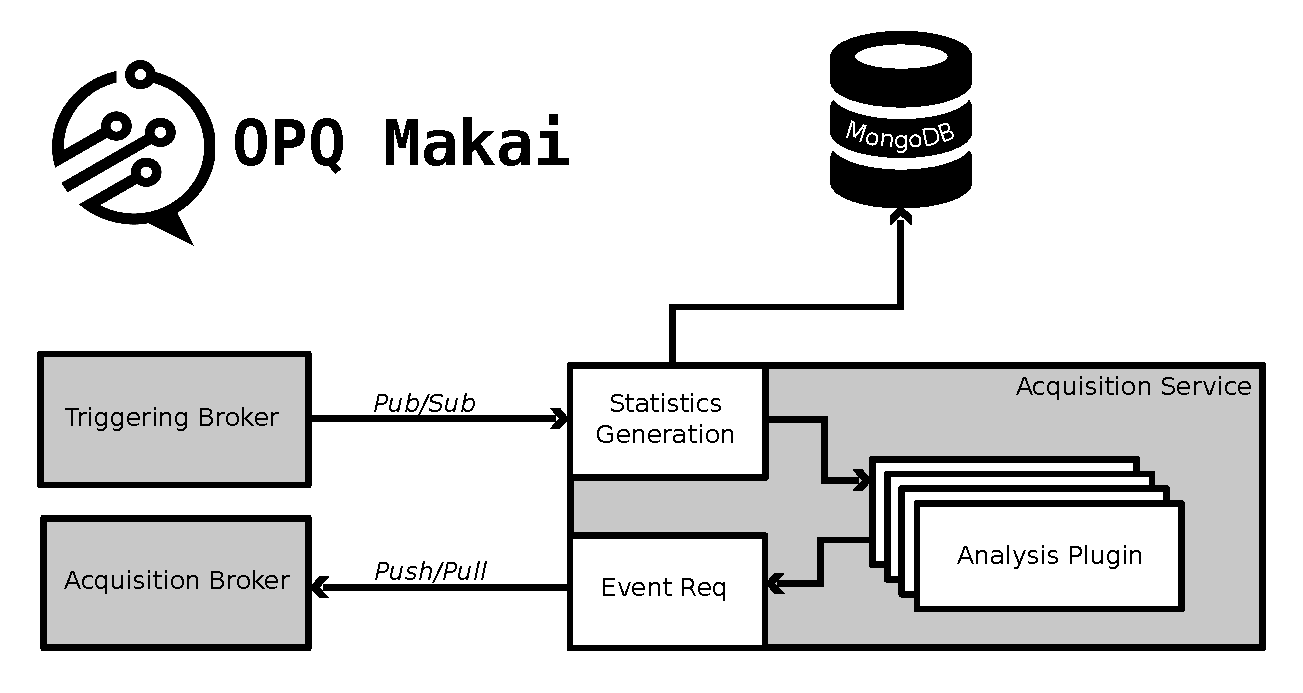
\includegraphics[width=0.6\textwidth]{img/makai_aqs.pdf}
	\end{center}
	\caption{Block diagram of the Acquisition Service.}
	\label{fig:opq:makai_aqs}
\end{figure}

\subsubsection{Triggering Stream Statistics.}

Acquisition Service accesses the triggering stream by connecting to the publish socket of the Triggering broker.
Since the connection is managed through the 0MQ publish-subscribe socket, several Acquisition Services can be connected to a single Triggering broker endpoint each servicing a subset of OPQ Boxes by subscribing to only specific devices.
This functionality is used to manage devices that the OPQ project sends to the mainland for evaluation by organisations interested in the project.
These loner devices participate in their own triggering schemes, and do not contaminate the triggering stream with messages about an unconnected grid.

Triggering messages received by the Acquisition service are buffered and stored in the mongo database.
There are two types of statistics accumulated by the Acquisition Service:
\begin{enumerate}
	\item \textit{Measurements:} Every triggering stream message gets converted to a set measurement.
	\item \textit{Trends:} One minute window of triggering stream messages get feature extracted and stored.
\end{enumerate}

Measurements have a one to one relationship with a triggering messages and take form of mongo documents described in Table \ref{tbl:opq:measurement_db}.
Measurement documents have an expire\_at field instructing Mongo to clean up the measurement collection after after a predetermined time period.
Currently measurement documents persist for 24 hours.
\begin{center}
	\begin{table}[!ht]
		\caption{Measurement Document.}
		\label{tbl:opq:measurement_db}
		\begin{tabularx}{\textwidth}[t]{ssb}
			\textbf{Field} & \textbf{Type} & \textbf{Description} \\
			\arrayrulecolor{black}\hline
			\textbf{box\_id} & \textit{string} & OPQ Box ID.\\
			\arrayrulecolor{black}\hline
			\textbf{timestamp\_ms} & \textit{uint64} & Millisecond timestamp.\\
			\arrayrulecolor{black}\hline
			\textbf{voltage} & \textit{f32} & $V_{rms}$ average value.\\
			\arrayrulecolor{black}\hline
			\textbf{thd} & \textit{f32} & THD average value\\
			\arrayrulecolor{black}\hline
			\textbf{frequency} & \textit{f32} & Frequency average value\\
			\arrayrulecolor{black}\hline
			\textbf{expire\_at} & \textit{f32} & Deletion time for the measurement.\\
		\end{tabularx}
	\end{table}
\end{center}

Trends consist of feature extracted statistics accumulated from 1 minute of triggering measurements
The statistic computed are minimum, maximum and average for each box metric.
Similarly to the Measurement documents, Trend documents expire after a predeterminned period of time.
Currently trends are retained for 7 days.
Structure of a Trend document is shown in Table \ref{tbl:opq:trend_db}.

\begin{center}
	\begin{table}[!ht]
		\caption{Trend Document.}
		\label{tbl:opq:trend_db}
		\begin{tabularx}{\textwidth}[t]{ssb}
			\arrayrulecolor{green}\hline
			\textbf{\textcolor{myGreen}{Trend Document}} & &\\
			\hline
			\textbf{Field} & \textbf{Type} & \textbf{Description} \\
			\arrayrulecolor{black}\hline
			\textbf{box\_id} & \textit{string} & OPQ Box ID.\\
			\arrayrulecolor{black}\hline
			\textbf{timestamp\_ms} & \textit{uint64} & Millisecond timestamp.\\
			\arrayrulecolor{black}\hline
			\textbf{voltage} & \textit{Statistics} & $V_{rms}$ average value.\\
			\arrayrulecolor{black}\hline
			\textbf{thd} & \textit{Statistics} & THD average value\\
			\arrayrulecolor{black}\hline
			\textbf{frequency} & \textit{Statistics} & Frequency average value\\
			\arrayrulecolor{black}\hline
			\textbf{expire\_at} & \textit{u64} & Deletion time for the measurement.\\
			& & \\
			\arrayrulecolor{green}\hline
			\textbf{\textcolor{myGreen}{Statistics}} & &\\
			\hline
			\textbf{Field} & \textbf{Type} & \textbf{Description} \\
			\arrayrulecolor{black}\hline
			\textbf{Min} & \textit{f32} & Minimum observed during the trend window.\\
			\arrayrulecolor{black}\hline
			\textbf{Max} & \textit{f32} & Maximum observed during the trend window.\\
			\arrayrulecolor{black}\hline
			\textbf{Average} & \textit{f32} & Average computed over the trend window.\\
			\arrayrulecolor{black}\hline
		\end{tabularx}
	\end{table}
\end{center}

\subsubsection{Triggering Analysis infrastructure.}

Acquisition Service does not include any analysis capabilities out of the box.
Instead analysis is performed by shared library loadable plugins.
These plugins can be loaded and unloaded at runtime, thus allowing live upgrading and testing of new analysis methods.
Plugin are loaded using libdl by searching for C function hooks which produce a Rust structure which implements a plugin interface.
The interface as well as the prototype C hook function are shown below:

\begin{lstlisting}[language=Rust, style=colouredRust]
pub trait MakaiPlugin: Any {
  fn name(&self) -> &'static str;
  fn process_measurement(&mut self, msg: Arc<Measurement>)->Option<Vec<Command>>;
  fn on_plugin_load(&mut self, json: String);
  fn on_plugin_unload(&mut self);
}
#[no_mangle]
pub extern "C" fn _plugin_create() -> *mut MakaiPlugin;

#[no_mangle]
pub extern "C" fn _plugin_destroy(plg : *mut MakaiPlugin);
\end{lstlisting}

The $\_plugin\_create$ function is marked as $no\_mangle$ which instructs the compiler to retain the function name so it can be located by the plugin loader.
It returns a mutable pointer to a boxed type which implements the MakaiPlugin interface.
Since Rust is a explicit memory management language, and the runtime is not aware of the internal structure of the Boxed type beyond it's interface,
a helper function $\_plugin\_destroy$ is used to cleanup the plugin object during the unloading process.
Each plugin runs in a separate thread with a synchronized queue from which it draws measurement messages.
If a plugins is not able to keep up with the triggering stream, Acquisition service will start dropping messages from it's input queue,
and a message indicating this fault will be stored in its log.
Once a plugin is loaded it will receive it's settings in form a of a json encoded string using the $on\_plugin\_load$ method.
This allows it to initialize all of the internal data structures to a known state.
Similarly $on\_plugin\_unload$ method is used to inform the plugin that it will be immanently unloaded.

The processing of the triggering stream occurs in the $process\_measurement$ method.
This methods takes a reference counted Measurement message in form shown in Table \ref{tbl:opq:trg_struct}.
Return type of this method is an optional list of commands to forward to the Acquisition broker in form shown in Table \ref{tbl:opq:cmd_struct}.
All of the Commands in the list are treated to be pertaining to the same event.

\subsubsection{Event Request.}
Once a plugin determines that an event of interest has taken place, it will emit a list of \textbf{RD} commands with structure shown in Table \ref{tbl:opq:cmd_payload}.
Event requester will fill in the identity field with the following string:
\[ identity = ``data\_" + EVENT\_TOKEN +"\_" + ACQ\_UUID\]

The ``$data\_$" prefix is used to route the messages responses from the OPQ Box to the Event storage service.
As mentioned previously, responses from device command need not return to the same service that sent the command.
Instead, the responses will be routed to a service which is subscribed to the identity used in the request.
The $EVENT\_TOKEN$ root is a 16 character random hexadecimal string, which identifies data request corresponding to the same event event.
Since a single event may contain data from multiple OPQ Boxes, and each event will have a unique $EVENT\_TOKEN$ root.
The $ACQ\_UUID$ postfix is used to identify the Acquisition service which triggered the data request.
Multiple Acquisition Services can be used to service the OPQ network, and each one is identified using it's own UUID identifier.
This identifier may be assigned to each service via the configuration file, or autogenerated at startup.
Once the identity of each command is filled in, each command is forwarded to the Acquisition broker for routing to the OPQ Box experiencing a power quality disturbance.

\subsection{Event Service.}\label{subsec:event-service}

Event service is a microservice which stores raw data generated by OPQ Boxes in the Mongo Database.
On initialization Event service queries mongo database for the highest event number recorded so far, connects to the Acquisition Broker's publish port,
and subscribes to all messages that start with the prefix ``$data\_$".
This allows the Event service to capture every response from OPQ Boxes generated from commands issued by the Acquisition service plugins.
Once the Event service receives a data response with an identity containing an $EVENT\_TOKEN$ it hasn't seen before it will increment the event number, and
store it in an internal key value store.
This way every future data message which contains that $EVENT\_TOKEN$, it will be appended to the same event.
Mongo ER diagram of the mongo event storage is shown in Figure \ref{fig:opq:mongo_er}.
Events collection contains metadata for individual events.
Box\_events collection contains metadata for event information from individual OPQ devices.
Finally gridfs, Mongo internal file storage, is used for storing event data.

\begin{figure}[h]
	\begin{center}
		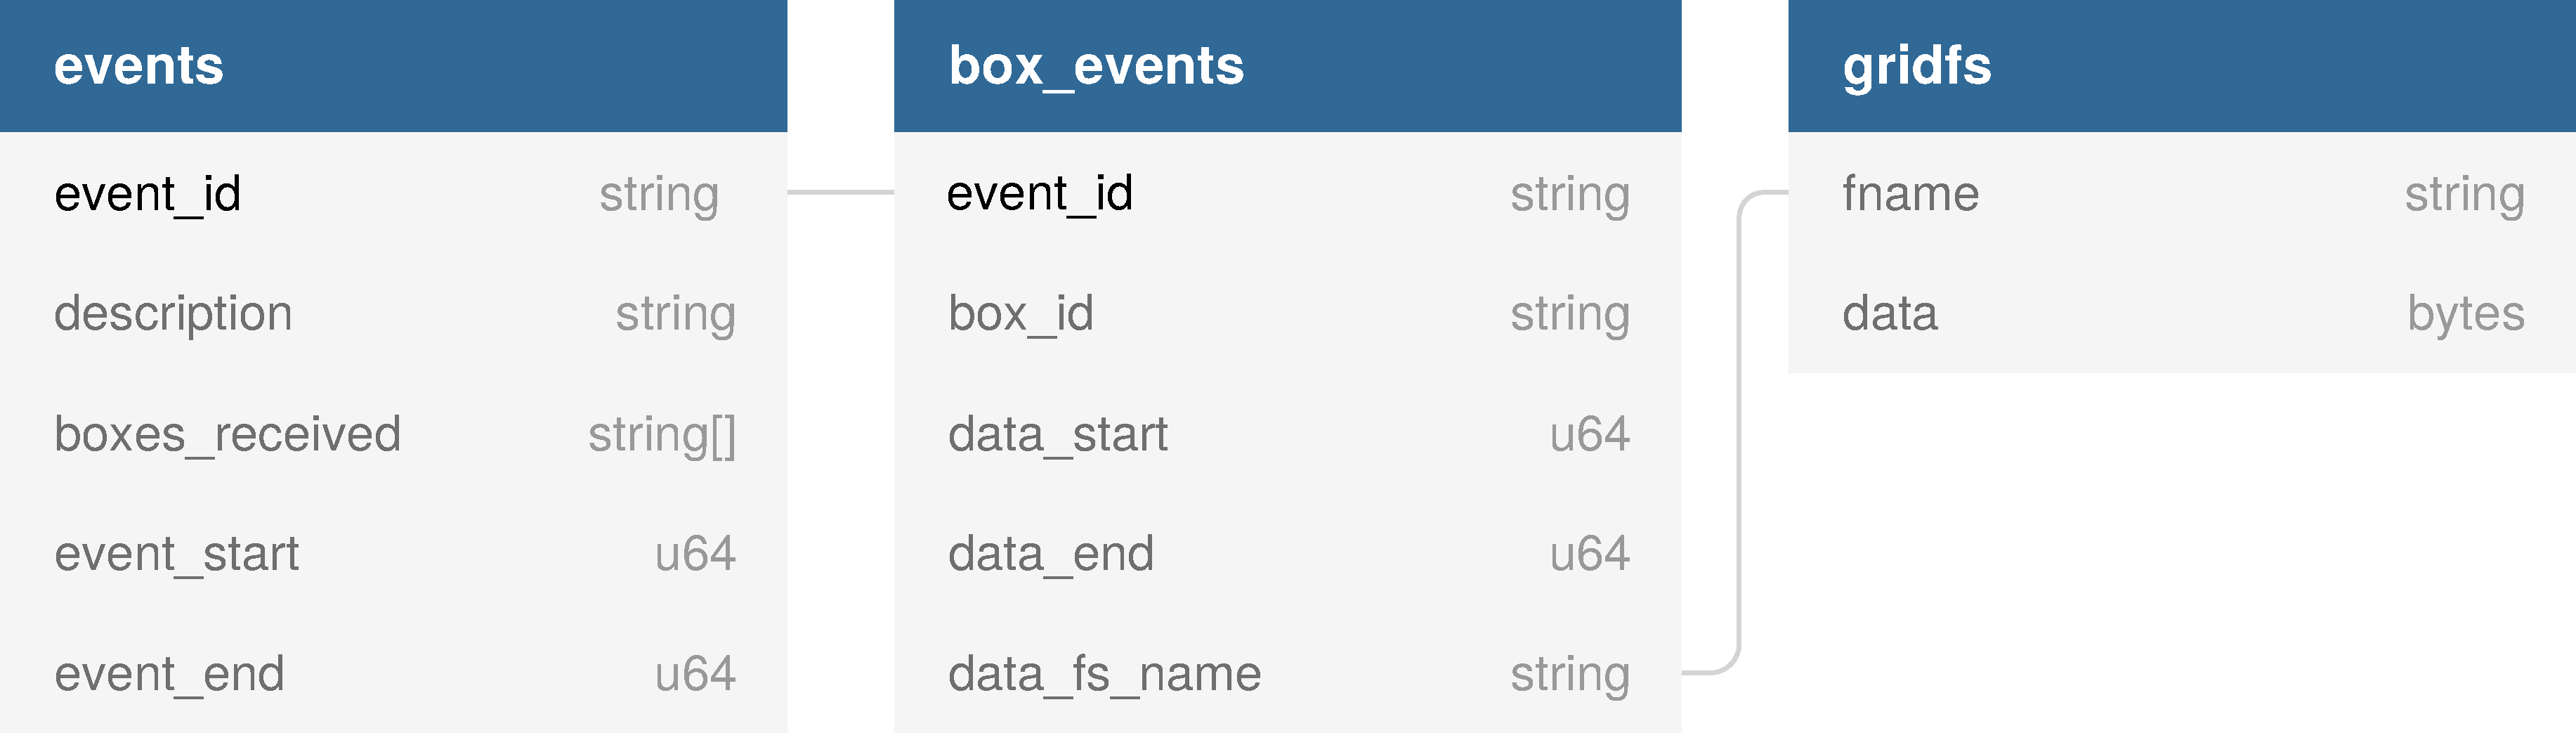
\includegraphics[width=0.9\textwidth]{img/mongo_event_storage.pdf}
	\end{center}
	\caption{ER diagram of event storage in Mongo DB}
	\label{fig:opq:mongo_er}
\end{figure}

\subsection{Acquisition Service Plugins}\label{subsec:acquisition-service-plugins}

Acquisition service plugins are responsible mor monitoring the OPQ Box triggering streams and determining when to request raw data.
A such Acquisition service plugins constitute the majority of business logic for the OPQ Makai system.
There are currently four plugins developed for this system:
\begin{enumerate}
	\item Health Plugin.
	\item Debug Plugin.
	\item Threshold Trigger.
	\item Napali Trigger.
\end{enumerate}

\subsubsection{Health Plugin}

The health plugin is responsible for monitoring the triggering messages passing through the Acquisition Service.
It maintains a REST endpoint for reporting the OPQ Network status.
Furthermore the REST endpoint can be used to trigger a device for debugging purposes.

\subsubsection{Debug Plugin}
Debug plugin consists of a Lisp interpreter which can manipulate the triggering stream, and emit triggering commands for devices.
It can be used to quickly and interactively test new analysis methods, and debug the OPQ network.

\subsubsection{Threshold Trigger}
Threshold trigger plugin is used for in situ comparison of a naive triggering method to Napali.
Every time the Threshold plugin receives a triggering message, it will check it against global thresholds.
If a metric value is outside of the predetermined thresholds the Triggering plugin will latch the timestamp and the id of the affected device.
Once the metric returns to normal, Threshold plugin will emit a request for raw data to the device which is experiencing an event.
If an event is longer then 50\% of the RDRB of an OPQ Box buffer an event will be broken up into several shorter events.
Threshold values for each metric are shown in Table \ref{tbl:opq:thresholds}

\begin{center}
	\begin{table}[!ht]
		\caption{Treshold values for each metric}
		\label{tbl:opq:thresholds}
		\begin{tabularx}{\textwidth}[t]{bss}
			\textbf{Metric} & \textbf{Min} &\textbf{Max}\\
			\arrayrulecolor{black}\hline
			$V_{rms}$ & $110V_{rms}$ & $120V_{rms}$ \\
			\arrayrulecolor{black}\hline
			$f_{fundamental}$ & $59.9Hz$ & $60.1Hz$ \\
			\arrayrulecolor{black}\hline
			$THD$ & N/A & $5\%$ \\
			\arrayrulecolor{black}\hline
			$Trans$ & N/A & $8V$ \\
		\end{tabularx}
	\end{table}
\end{center}


Threshold Trigger plugin functions in the same way as a self-triggering device.
Since this method of event detection does not rely on intra-box information sharing, it functions in the same manner as if the OPQ Box itself
is performing event detection.
This allows for experimental comparison of the Napali method efficiency with the self-triggered methodology.

\subsubsection{Napali Trigger}\label{subsec:napali-trigger}

Napali Trigger plugin implements the Napali event detection method.
Napali Trigger state machine is kicked off the same way as the Threshold trigger.
If a received metric value is outside of the predetermined thresholds Napali plugin will latch the timestamp and the id of the affected device.
Similarly, once the offending metric from all devices return to normal, Napali plugin will emit a request for raw data to the device which is experiencing an event.
The main difference between the Napali trigger and the Threshold trigger are two-fold:
\begin{enumerate}
	\item An event is not considered finished until every device's metrics return to the nominal threshold range.
	\item Metric value is within the nominal threshold but outside 3 standard deviations of a mean, will cause a the device to be participating in the  event.
\end{enumerate}

The first difference allows Napali to track a propagation of a fault throughout the power delivery network.
Furthermore, during a lifetime of a power quality event, it may shift from one metric to another.
As the disturbance travels, through the power-grid, Napali will aggregate all of the temporally localized disturbances into one event.
The second disturbance allows for recording of sub-threshold data to be acquired from devices which did not pass the threshold, but exhibited anomalous behaviour.

The mean and standard deviation are calculated using two first order IIR filter loops as show in Equation \ref{eq:fir_mean}:
\begin{equation}\label{eq:fir_mean}
\begin{aligned}
	\mu_{n+1} = (1- \alpha)*\mu_{n} + \alpha * m \\
	\mu^2_{n+1} = (1- \alpha)*\mu^2_n + \alpha * m^2 \\
	\sigma^2_n = \mu^2_n - (\mu_n)^2 \\
	\sigma_n =\sqrt{\sigma_n^2}
\end{aligned}
\end{equation}
Where $\mu$ is the mean, $\sigma$ is the standard deviation, $m$ is the new sample and $\alpha$ is the decay parameter.
Notice that $(\mu)^2$ is the square of the mean, and $\mu^2$ is the mean of the squares.
The $\alpha$ parameter determines the memory of the filter, and can be computed as:
\begin{equation}\label{eq:fir_alpha}
\begin{aligned}
	\alpha = 1 - e^{2\pi\frac{T_{sample}}{T_{memory}}}
\end{aligned}
\end{equation}
Where $T_{sample}$ is the sampling rate of the system, 1s for OPQ, and $T_{memory}$ is the desired response of the system.

Using an IIR filter for mean and standard deviation calculation is computational cheaper then using a FIR window.
Furthermore, using the IIR filter makes it trivial to tune the response of the system during runtime.

\section{OPQ Mauka}\label{sec:opq-mauka}
OPQ Mauka service is responsible for higher level classification and filtering of the anomalies generated by the OPQ Makai.
Since anomalies generation only
relies on the triggering stream features and not raw data, OPQ Makai is not able to ascertain if the anomaly is an actual power quality event, event type, or its severity.
OPQ Mauka on the other hand operates on the raw data, thus it is able to perform high level analysis to meet industry standards for vent classification.
The block diagram of the OPQ Mauka is shown in~\ref{fig:opq:11}.
\begin{figure}[h]
  \begin{center}
  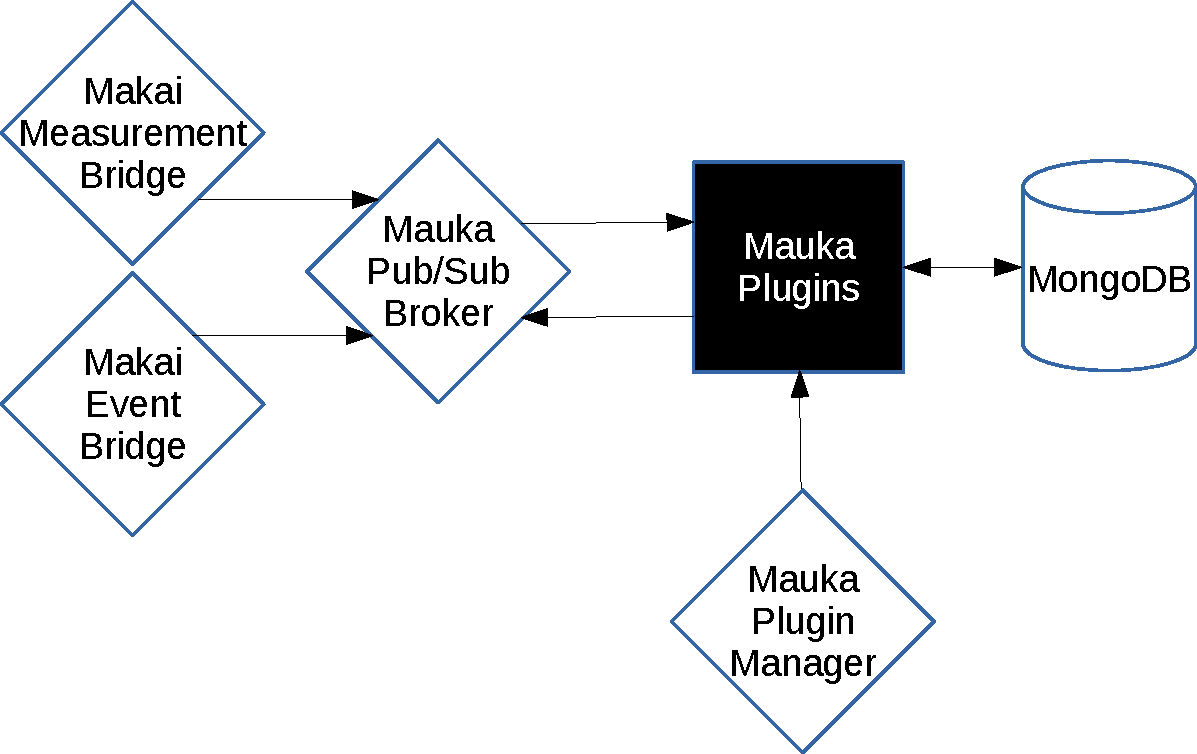
\includegraphics[width=0.6\textwidth]{img/mauka.pdf}
  \end{center}
  \caption{Block diagram of the OPQ Mauka.}
  \label{fig:opq:11}
\end{figure}

Currently OPQ Mauka supports the following classification strategies:
\begin{itemize}
	\item{\textbf{ITIC}} Power acceptability curve used to classify short term voltage sags.
	\item{\textbf{IEEE 1159 Voltage}} Voltage classification based on the IEEE 1159 power quality standard.
	\item{\textbf{Brownout Detection}} Classification of medium to long term voltage sags.
	\item{\textbf{Total Harmonic distortion}} Classification of events via harmonic analysis.
\end{itemize}

Once the anomaly is classified by OPQ Mauka, and the power quality characteristics are confirmed, it may be aggregated with other anomalies to form a disturbance.
Disturbances are composed of raw box data, analysis results as well as expert annotations and other metadata.

\section{OPQ View}\label{sec:opq-view}

OPQ View is the primary user interface to the OPQ ecosystem.
View is written in JavaScript using the Meteor framework, and provides a robust and easy to use interface to the OPQ Box triggering stream, Makai triggering anomalies, and to the Mauka PQ disturbances.
Furthermore, View provides an administration interface for initial setup and maintenance of the OPQ devices, and services.
Finally OPQ View monitors the health of the OPQ components, keeping track of the individual box uptimes, and component failures.
A screenshot of the recent OPQ View build is shown in Figure~\ref{fig:opq:12}

\begin{figure}[h]
  \begin{center}
  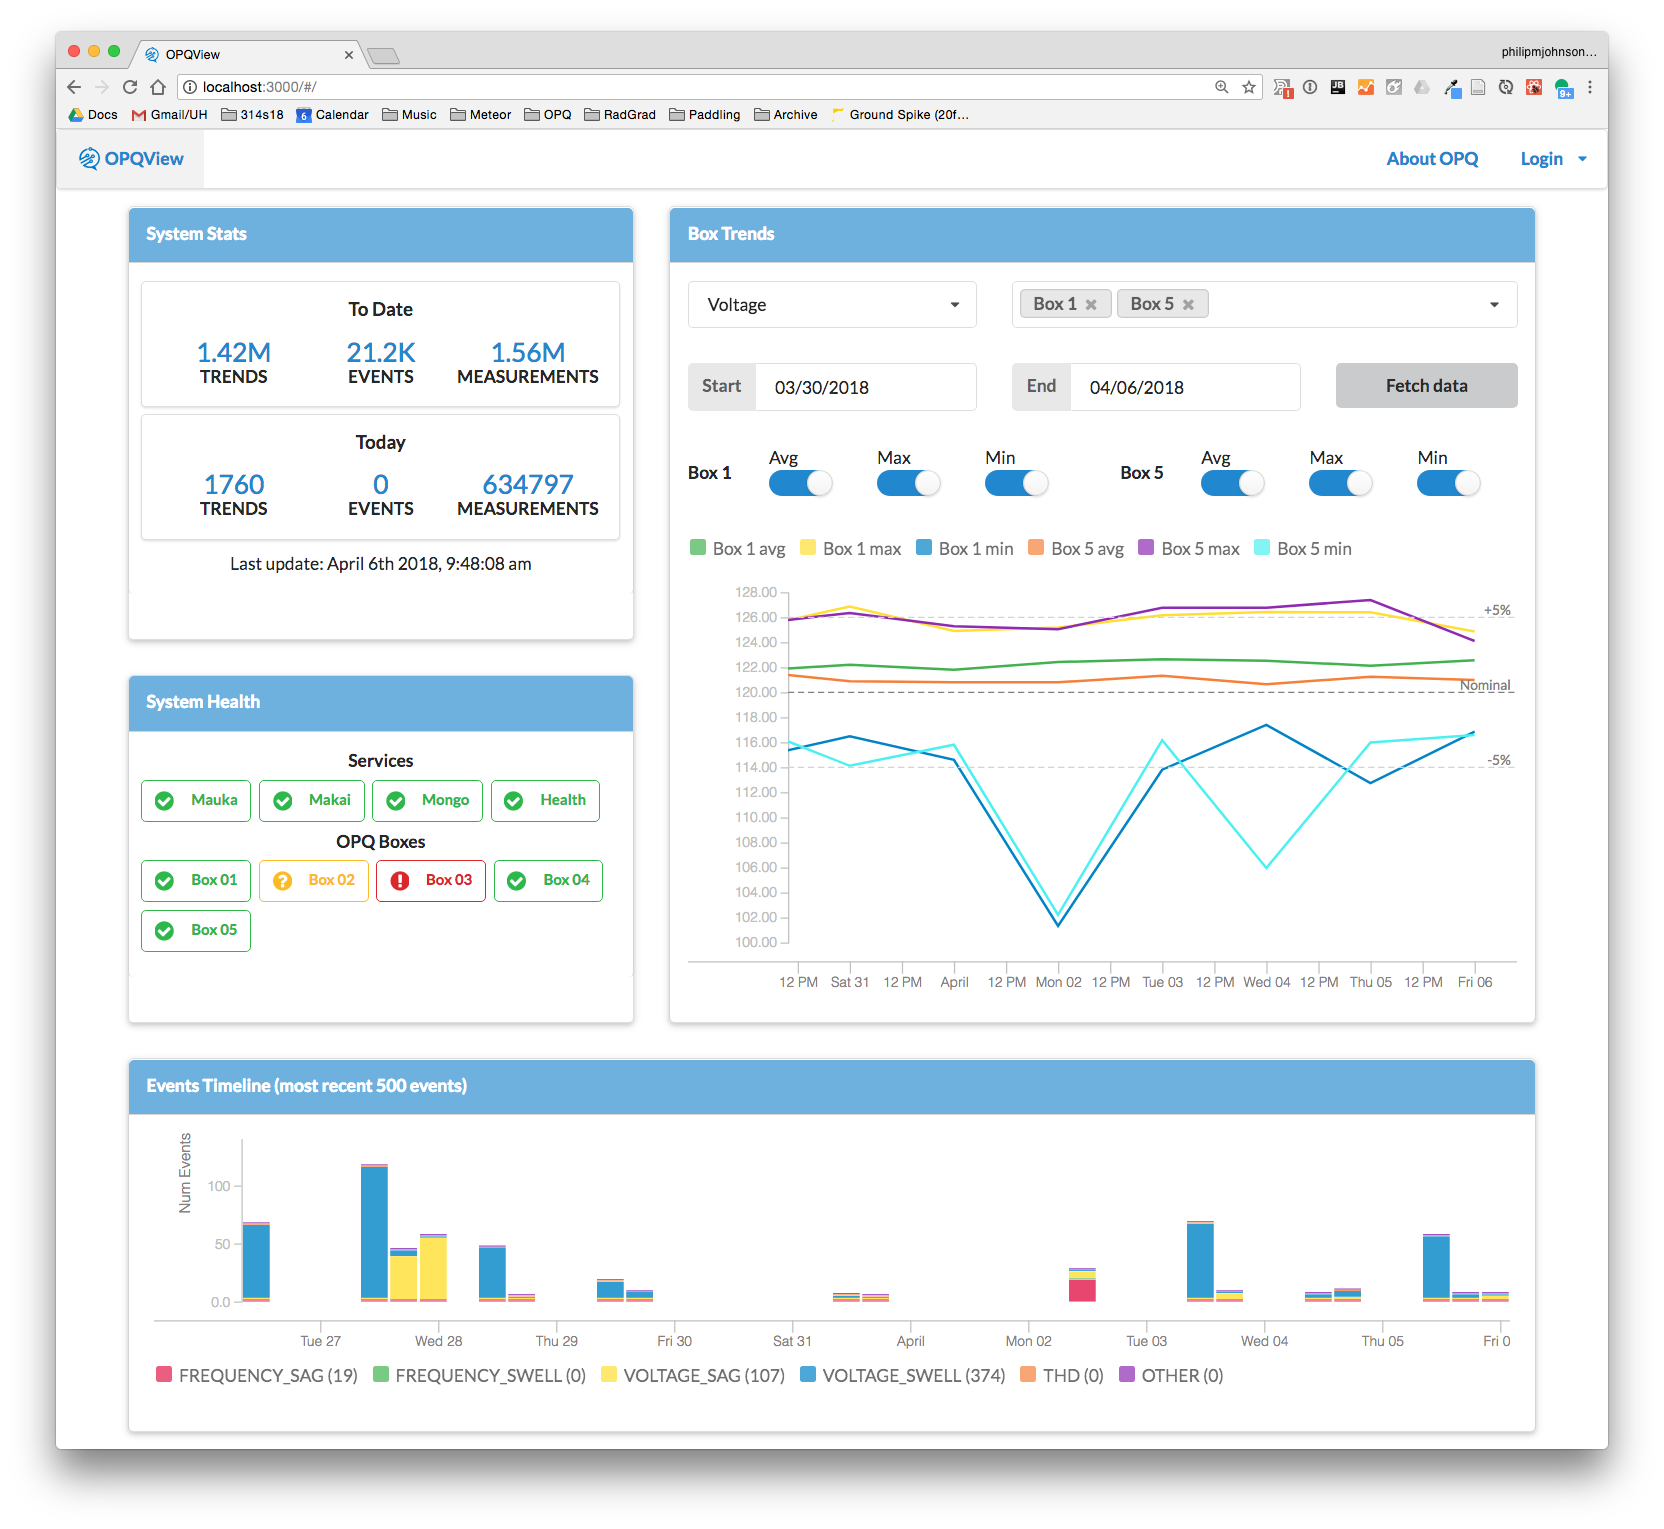
\includegraphics[width=0.6\textwidth]{img/opqview-landing-page.png}
  \end{center}
  \caption{Screenshot of a recent OPQ View build.}
  \label{fig:opq:12}
\end{figure}


\chapter{Experiment Description}
Validation of the Napali approach is intrinsically linked to validation of Makai, both with synthetic benchmarks and in-situ.
Since OPQ utilizes a custom power quality measurement device, its performance needed to be characterized prior to Makai evaluation.

\section{OPQ Box Characterization.}\label{sec:opq-box-characterization.}
A mentioned in Section~\ref{subsec:software} OPQBox generates 4 metrics in order to enable event detection.
In order to evaluate the limits of detection capabilities for each one of these metrics, an OPQBox was fed with synthetic waveform generated by the SDG1025 function generator.
By utilizing a function generator the entire device including the hardware analog front end could be evaluated.
Since the function generator is not capable of supplying $120V_{rms}$ signal, a $120mV_{rms}$ signal was fed on a low side of the OPQBox resistor divider, while the device was powered via an external 5V power supply.

\subsection{Fundamental Frequency}

Fundamental Frequency computation was evaluated by generating a 60Hz sine wave via the SDG1025 and supplying it to the OPQBox.
Calculated frequency was accumulated by analyzing the device triggering stream.
The resulting histogram is shown in Figure~\ref{fig:expdes:1}
\begin{figure}[H]
    \begin{center}
        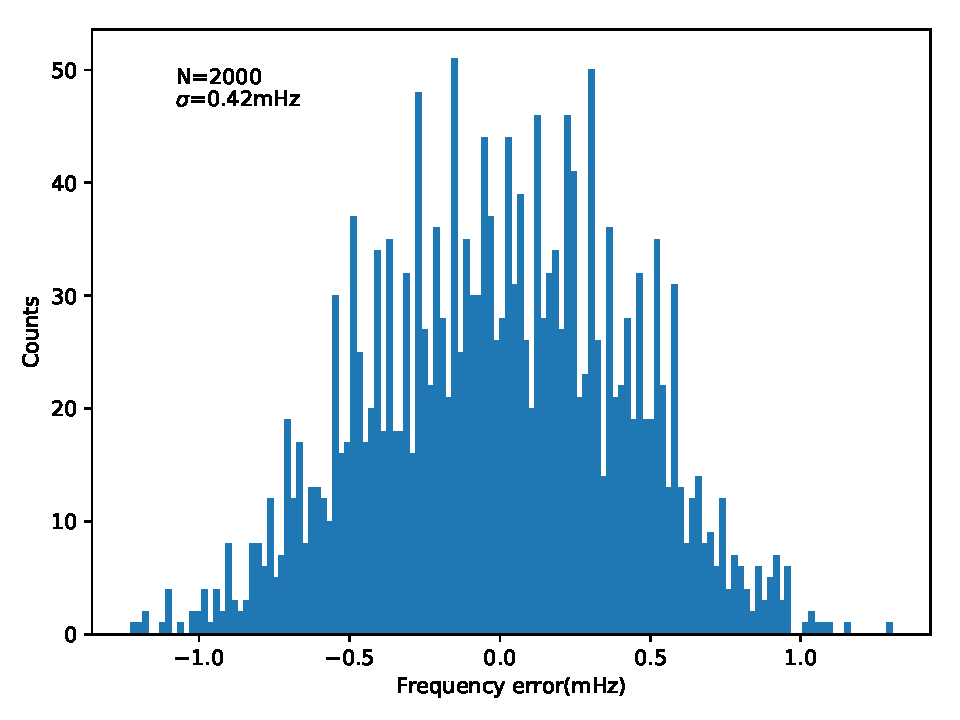
\includegraphics[width=0.6\textwidth]{img/box_eval/frequency_rms.pdf}
    \end{center}
    \caption{OPQBox frequency response.}
    \label{fig:expdes:1}
\end{figure}
As shown, the resulting distribution collected frequencies acquired over 2000s has a $\sigma=420uHz$.

\subsection{Root Mean Square Voltage}
Similarly to the fundamental frequency characterization, $V_{rms}$ calculation was evaluated by supplying the OPQBox with a 60Hz, $120mV_{rms}$ sine wave via the SDG1025.
Calculated RMS was accumulated by analyzing the device triggering stream.
The resulting histogram is shown in Figure~\ref{fig:expdes:2}

\begin{figure}[h]
    \begin{center}
        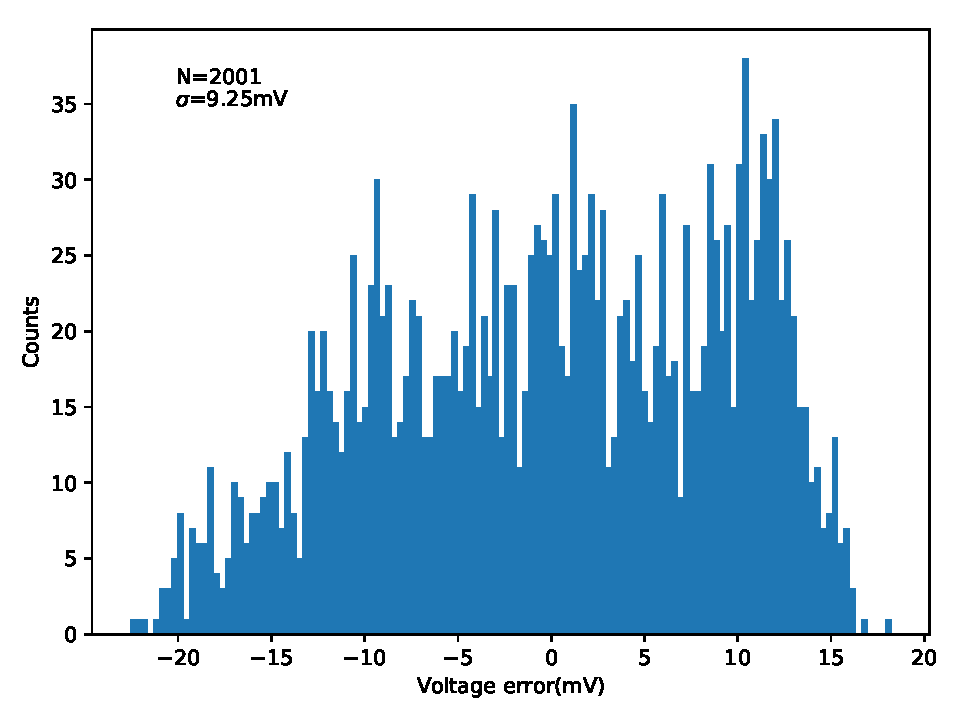
\includegraphics[width=0.6\textwidth]{img/box_eval/rms_histogram.pdf}
    \end{center}
    \caption{OPQBox $V_{rms}$ response.}
    \label{fig:expdes:2}
\end{figure}

As shown, the resulting distribution of collected $V_{rms}$ measurements, acquired over 2000s has a $\sigma=9.34mV$

\subsection{Total Harmonic Distortion}

THD performance of the OPQBox was validated by injecting a various harmonics of 60Hz superimposed onto the 60Hz, $120mV_{rms}$ sine wave into the device via the SDG1025 arbitrary waveform generation capability.
THD calculation results were acquired from the OPQBox triggering stream for analysis.
As expected resultant performance remained self-consistent across all harmonics.
Figure~\ref{fig:expdes:3} shows a histogram of the error in THD values computed form a 60Hz, $120mV_{rms}$ sinewave superimposed with a 240Hz $1.2mV_{rms}$ sine wave.
This measurement is equivalent to $1\%$ THD at the $4^{th}$ harmonic.

\begin{figure}[h]
    \begin{center}
        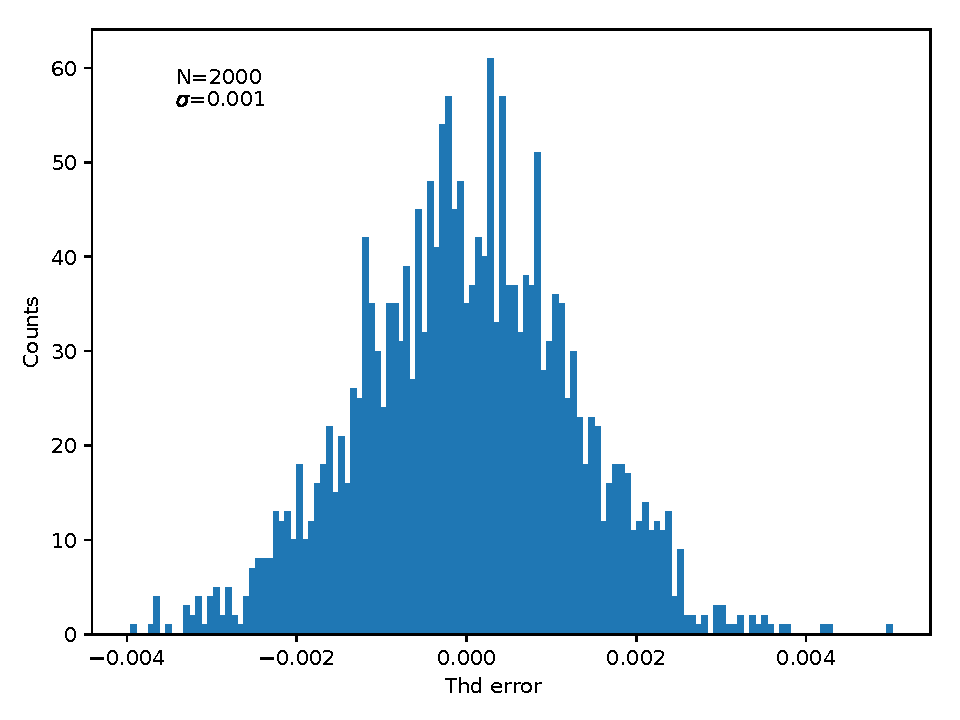
\includegraphics[width=0.6\textwidth]{img/box_eval/thd_rms.pdf}
    \end{center}
    \caption{OPQBox THD response.}
    \label{fig:expdes:3}
\end{figure}

As shown, the resulting distribution of collected THD measurements, acquired over 2000s has a $\sigma=0.001\%$.

\subsection{Transient Detection}

Transient detection performance was evaluated by injecting a transient superimposed onto the 60Hz, $120mV_{rms}$ sine wave into the device via the SDG1025 arbitrary function generation capability.
Transient detection results were acquired by capturing and analyzing the device triggering stream.
Transients of various shapes and magnitudes were tested.

\begin{figure}[h]
    \centering
    \begin{subfigure}{.5\textwidth}
        \centering
        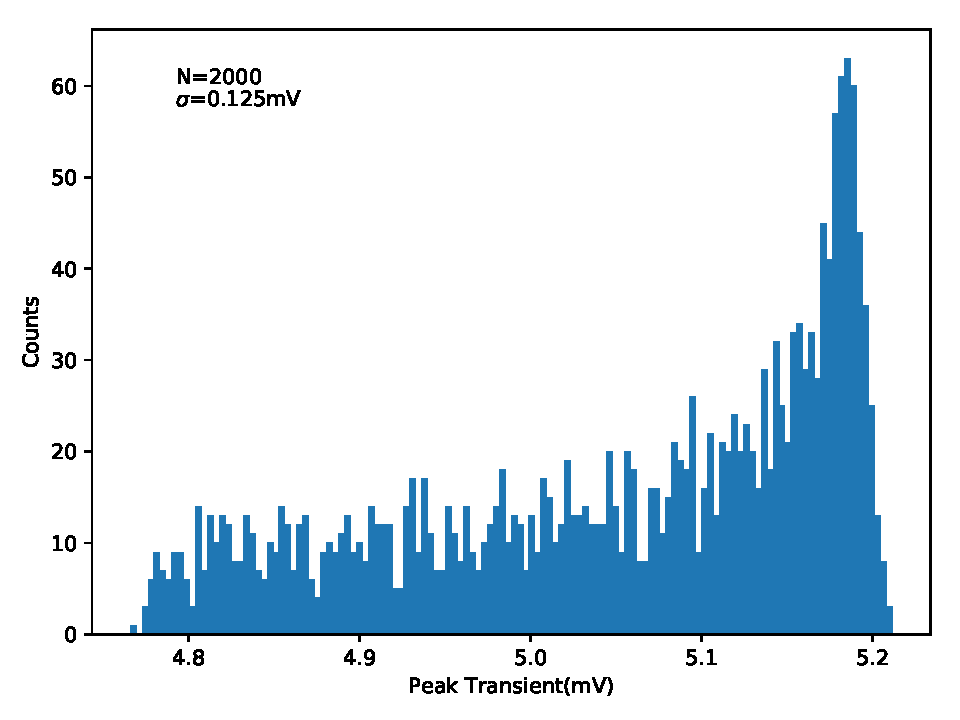
\includegraphics[width=0.9\linewidth]{img/box_eval/5v_transient_rms.pdf}
        \caption{}
        \label{fig:expdes:4:1}
    \end{subfigure}%
    \begin{subfigure}{.5\textwidth}
        \centering
        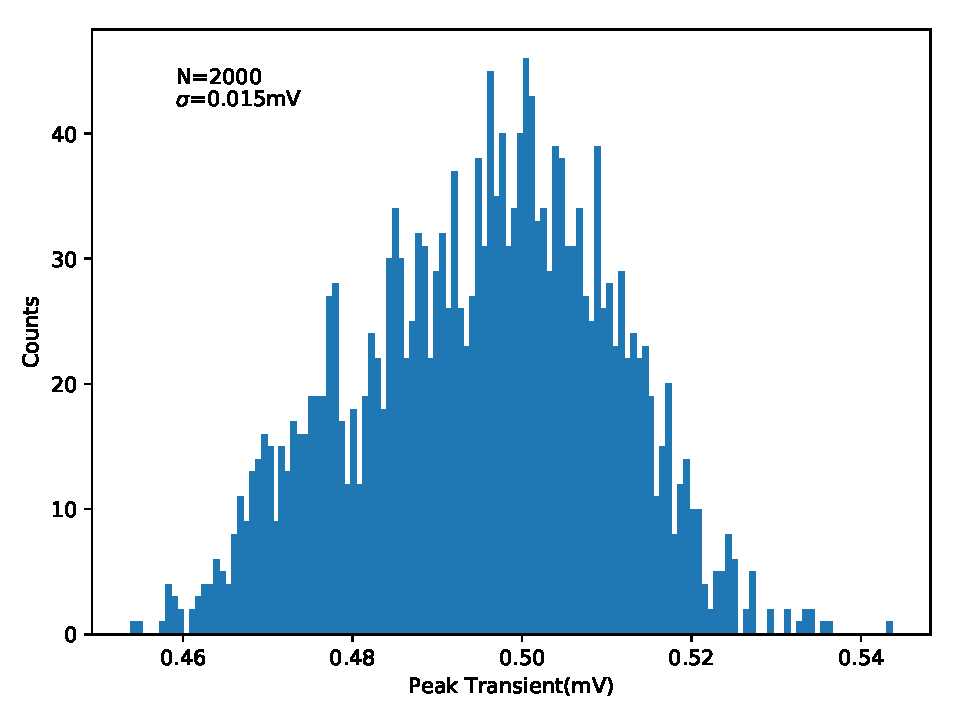
\includegraphics[width=0.9\linewidth]{img/box_eval/0p5v_transient_rms.pdf}
        \caption{}
        \label{fig:expdes:4:2}
    \end{subfigure}
    \caption{Transient detection metric with a 5V transient(a), and 0.5V transient(b)}
    \label{fig:expdes:4}
\end{figure}

Figure~\ref{fig:expdes:4} shows the resultant transient detection metric for two transients.
The shape of the transient is the same and is shown in Figure~\ref{fig:opq:8:3}.
Interestingly, in case of a 0.5V transient the metric results in a much tighter distribution with $\sigma =0.015V$, while in the case of
a 5V transient the distribution exhibits a lower sideband tail.
Since the transient is injected in a random position in the cycle, and the sampling rate of the DG1025 is significantly higher then sampling rate of the OPQBox(25Msps vs 12Ksps), the peak of the transient will sometimes fall in between the consecutive samples of the OPQBox.
In the $0.5V$ transient case this effect is alleviated, since the transient is so small.
Regardless, the result shown in Figure~\ref{fig:expdes:4:2} is presented only as a synthetic benchmark, since OPQBox is expected to operate in an environment with THD larger then $0.4\%$ at $>400Hz$ required to detect a $0.5V$ transient.
As such, the figure of $\sigma=0.125V$ should be considered valid for the OPQBox transient detection capability.
Since this metric is only used in transient detection and not characterization, it was found to be sufficient.

\section{Napali Validation}\label{sec:napali-validation.}
Napali method was validated using simulation, synthetic data with the device-in-loop, and in-situ during the deployment.
The main tunable parameter in the napali is the $\alpha$ coefficient used in the low pass filter as shown in Equation \ref{eq:iir_mean}.
This parameter determines the memory of the lowpass filter used in the calculation of the mean and the standard deviation of metrics from OPQBox data stream.
These statistics are in turn used during the Napali triggering process to locate sub-threshold gridwide events.

\subsection{Selection of $\alpha$ parameter}\label{subsec:selectrion-ofparameter}
Smaller $\alpha$ parameter corresponds to a longer memory in the low pass filter as shown in Equation \ref{eq:iir_alpha}.
This is further visualized in Figure \ref{fig:expdes:5}.
In particular this Figures \ref{fig:expdes:5:1} and \ref{fig:expdes:5:2} show the response of the IIR low pass filter to the simulated frequency measurements.
The dashed red line represents the frequency measurement, solid red line represents the filtered mean, and the blue line represents the standard diviation.
Figures \ref{fig:expdes:5:1} shows the filter response for $\alpha = 0.5$ or $T_{memory} \approx 10s $.
As evident from the plot, the mean and the standard deviation quickly recover from the transient are return to their nominal values.
Furthermore, the mean is closely tracking the random fluctuations present in the measurement.
Figures \ref{fig:expdes:5:1} shows the filter response for $\alpha = 0.05$ or $T_{memory} \approx 123s $.
While the stimuli remains the same, it takes significantly longer the statistics to recover.
Additionally, the mean no longer tracks the frequency fluctuations present in the simulated data.

\begin{figure}[h]
    \centering
    \begin{subfigure}{0.9\textwidth}
        \centering
        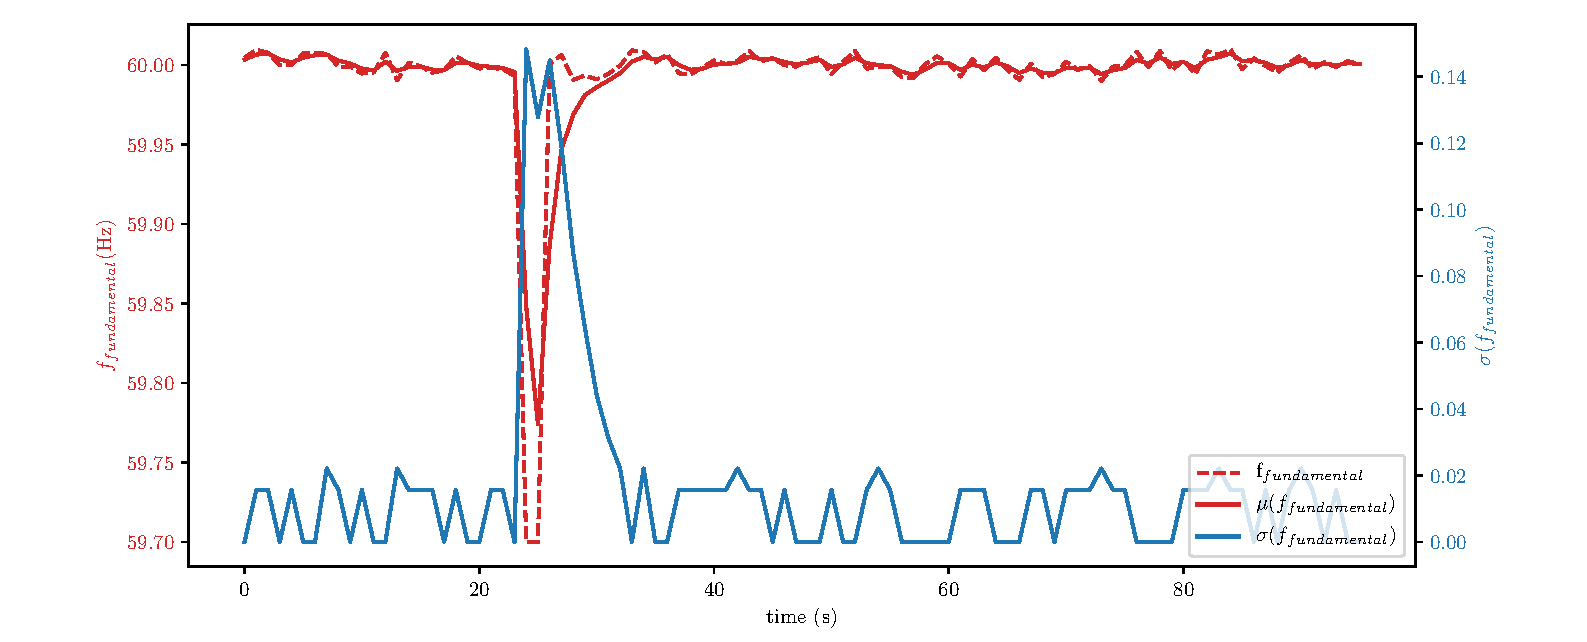
\includegraphics[width=1\linewidth]{img/napali_eval/Napali_response_freq_05.pdf}
        \caption{}
        \label{fig:expdes:5:1}
    \end{subfigure}%

    \begin{subfigure}{0.9\textwidth}
        \centering
        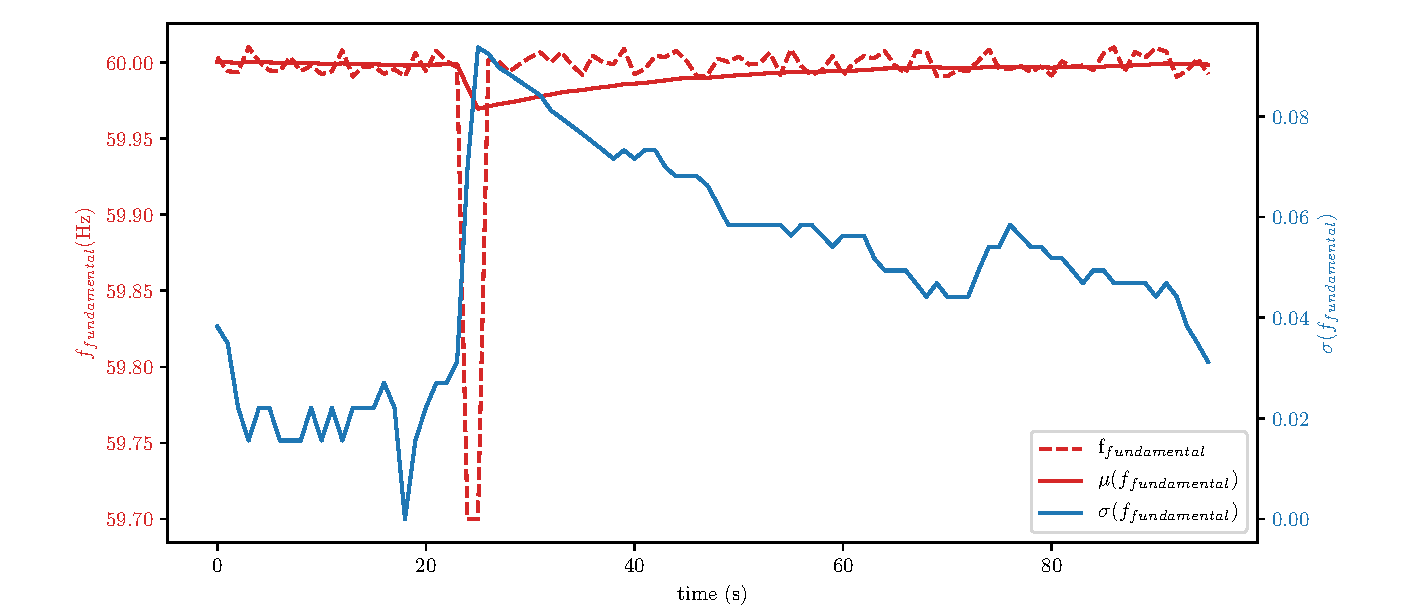
\includegraphics[width=1\linewidth]{img/napali_eval/Napali_response_freq_005.pdf}
        \caption{}
        \label{fig:expdes:5:2}
    \end{subfigure}
    \caption{$\mu$ and $\sigma$ behaviour with a)$\alpha = 0.5$ and b)$\alpha=0.05$}
    \label{fig:expdes:5}
\end{figure}

Picking the $\alpha$ parameter for Napali is extremely domain specific, as it depends on the frequency content of the triggering stream.
Intuitively, the $T_{memory}$ parameter needs to be long enough to adjust to gradual changes in the triggering stream for the mean calculation,
and dampen the standard deviation for detection of multiple consecutive anomalies.
In addition, it needs to be short enough to converge on the mean and the standard deviation during a step-like transition in the triggering stream.

Luckily, in the Power Quality domain the Napali $\alpha$ selection is fairly forgiving.
This is demonstrated in Figure \ref{fig:expdes:6}.
This graph represents the amount of time that Napali considered one of the metrics to be outside of the $3\sigma$ of the mean for various values of $\alpha$.
The triggering stream used to generate these values was captured over 24 hours by one of the OPQBoxes deployed on the University of Hawaii campus.
All devices deployed thus far have followed a similar pattern.
With $200s <T_{memory} < 2Hr$ the triggering stream resulted in similar behaviour, with the system correctly marking all potential sub-threshold events.
At $T_{memory} \approx 500s$, system quickly recovered from large jumps in the triggering stream, however it marked a significant number of small anomalies ($\Delta_{f}>0.01Hz$, $\Delta_{v}> 0.1V$\ldots etc) as outside $3\sigma$, and thus candidates for sub-threshold events.
At $T_{memory} \approx 2Hr$, system took  significant amount of time to recover from large jumps in triggering metrics, thus marking the metric as outside of $3\sigma$ for many tens of minutes.
Furthermore, some of the larger anomalous measurements ($\Delta_{f}>0.05Hz$, $\Delta_{v}> 2V$\ldots etc) were no longer flagged as sub-threshold candidates.
Outside of the two extremes, the system behaviour was quite similar.
During all of the deployments the OPQ system was operating with:
\begin{equation}\label{eq:opq_alpha}
\begin{aligned}
    \alpha = 0.005
\end{aligned}
\end{equation}


Which corresponds to the $T_{memory} \approx 21$ minutes.
Thresholds which initiate the Napali event detection state machine are shown in Table \ref{tbl:opq:thresholds}.

\begin{figure}[h]
    \centering
        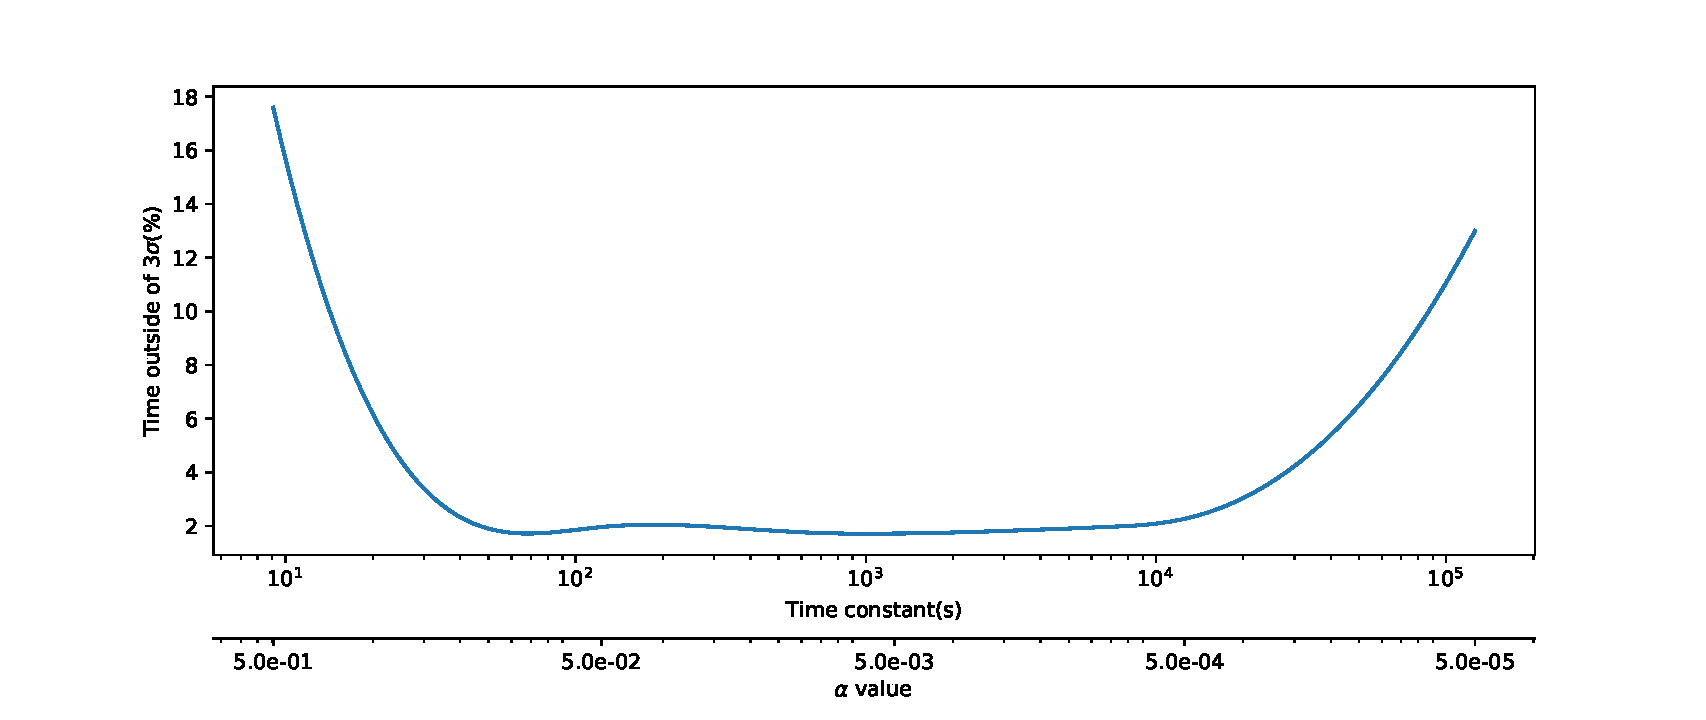
\includegraphics[width=1\linewidth]{img/napali_eval/a_selection.pdf}
    \caption{Amount of time a metric spends outside of the $3\sigma$ for various values of $\alpha$}
    \label{fig:expdes:6}
\end{figure}

The effect of the of selecting alpha as shown in Equation \ref{eq:opq_alpha} can be observed in Figure \ref{fig:expdes:7}.
This figure shows interesting features form the same dataset that was used to produce Figure \ref{fig:expdes:6}.
Blue traces show metrics that exhibit anomalous behaviour, while red indicates that Napali has flagged this temporal region as a sub-threshold event candidate.
Figure \ref{fig:expdes:7:1} shows a frequency fluctuation which nearly passes the threshold of $60.1Hz$ which would mark it as a full fledged event.
Instead, Napali marked almost the entirety of the fluctuation as a potential sub-threshold event, as shown by the red trace.
Figure \ref{fig:expdes:7:2} shows a step in the total harmonic distortion metric, similar to the one shown in Figure \ref{fig:opq:7} at the 6am mark.
In this case the metric in question abruptly changed to a new mean, requiring a fairly slow $\alpha$ coefficient to catch up over 3 minutes.
While it may seem wasteful to mark large temporal regions following an abrupt jump as candidates for sub-threshold event, it is important to note that:
\begin{enumerate}
    \item Making the $\alpha$ parameter smaller does not benefit the false positive rate as shown in Figure \ref{fig:expdes:6}.
    \item In-situ there is no way to tell if an abrupt shift is a switch to a new steady state, or if the metric will recover to a previous mean.
\end{enumerate}
It is important to remember than Napali is not meant to have a low false positive rate.
Instead, a system like OPQ Mauka can use all available information, including the raw data, to determine if an event is true gridwide event with much higher confidence.
The main goal of Napali is to have an extremely low rate of false negatives.
Figure \ref{fig:expdes:7:3} is on a different timescale from Figures \ref{fig:expdes:7:2} and \ref{fig:expdes:7:1}.
This is done in order to include several potential sub-threshold events into a common chart.
Five temporal regions during the the 3 Hrs are marked by Napali as potential sub-threshold events.
\begin{figure}[h]
    \centering
    \begin{subfigure}{0.5\textwidth}
        \centering
        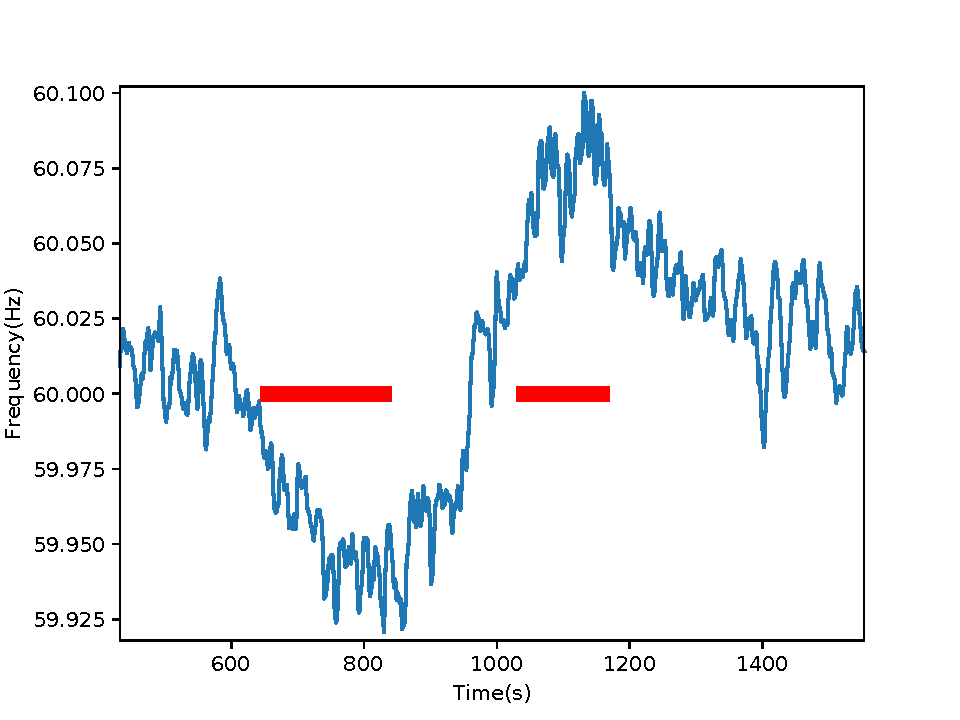
\includegraphics[width=1\linewidth]{img/napali_eval/napali_live_f.pdf}
        \caption{}
        \label{fig:expdes:7:1}
    \end{subfigure}%
    \begin{subfigure}{0.5\textwidth}
        \centering
        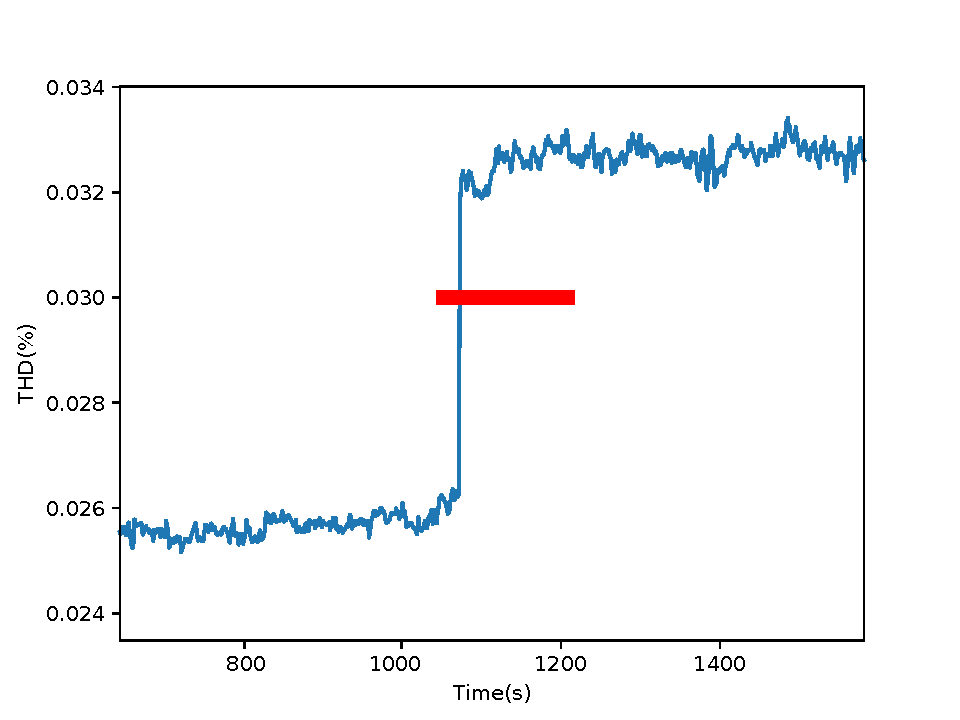
\includegraphics[width=1\linewidth]{img/napali_eval/napali_live_thd.pdf}
        \caption{}
        \label{fig:expdes:7:2}
    \end{subfigure}

    \begin{subfigure}{0.5\textwidth}
        \centering
        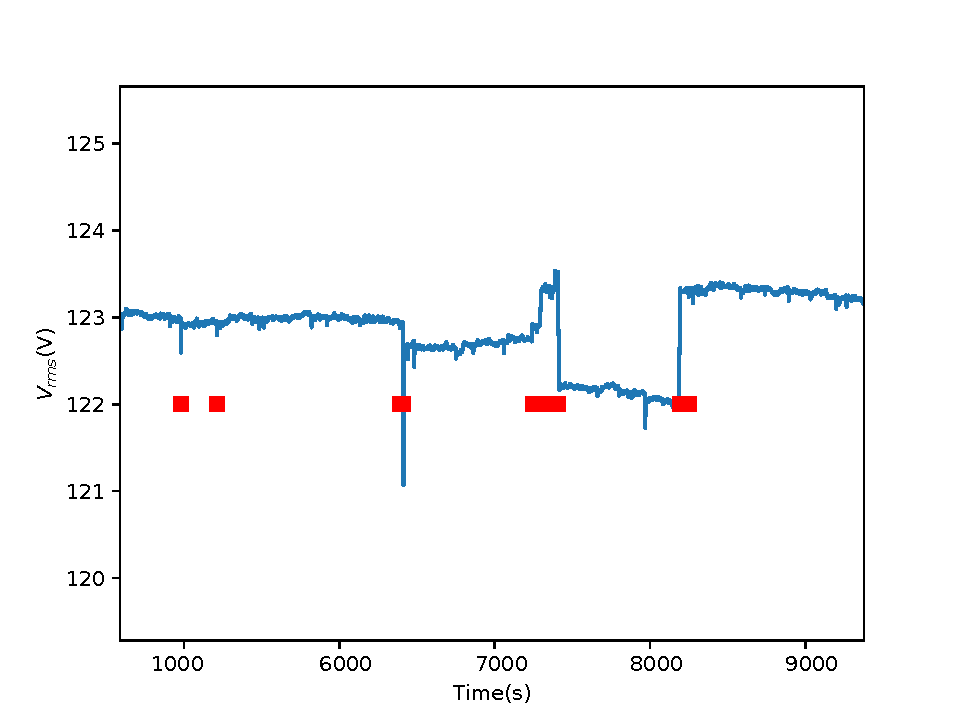
\includegraphics[width=1\linewidth]{img/napali_eval/napali_live_rms.pdf}
        \caption{}
        \label{fig:expdes:7:3}
    \end{subfigure}%
    \begin{subfigure}{0.5\textwidth}
        \centering
        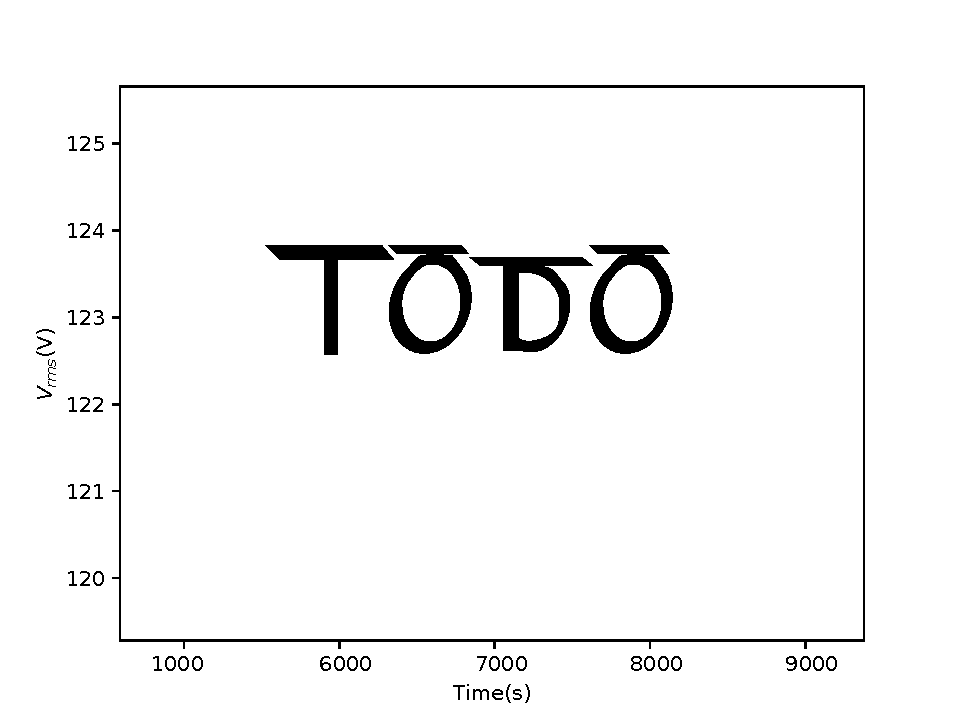
\includegraphics[width=1\linewidth]{img/napali_eval/napali_live_trans.pdf}
        \caption{}
        \label{fig:expdes:7:4}
    \end{subfigure}

    \caption{Potential sub-threshold events for a) $f_{fundamental}$, b)$THD$, c)$V_{rms}$ and d)$Trans$.
    Red boxes indicate that Napali picked these temporal windows as a potential sub-threshold event.}
    \label{fig:expdes:7}
\end{figure}

\subsection{Sub-Threshold Event Detection}\label{subsec:sub-threshold-event-detection}

One of the main goals of Napali is to utilize metric extraction in order to detect sub-threshold events.
During the deployment, two types of subthreshold events have been identified:
\begin{itemize}
    \item Partial sub-threshold event.
    \item Full sub-threshold event.
\end{itemize}
Full sub-threshold events consist of one or several devices passing the threshold described in Table \ref{tbl:opq:thresholds},
as well as one or several devices marked as sub-threshold by Napali.
Partial sub-threshold events consist of devices which all passed the threshold described in Table \ref{tbl:opq:thresholds}, however some of the devices triggered on a different metric with a much shorter temporal window.
The important distinction between partial sub-threshold events and regular events is that if triggered using the self-triggering method, the majority of the sub-threshold data would be lost.

\begin{figure}[h]
    \centering
    \begin{subfigure}{1\textwidth}
        \centering
        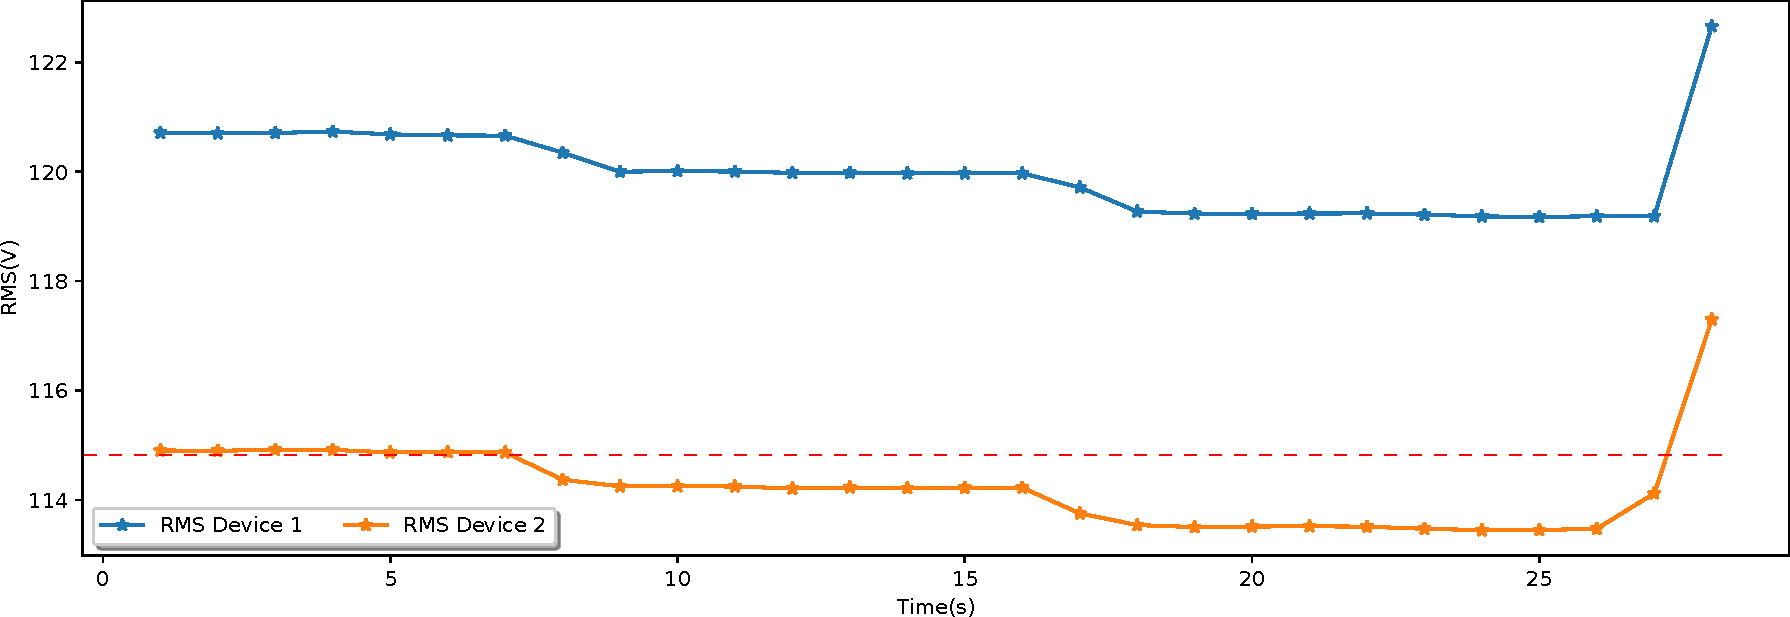
\includegraphics[width=1\linewidth]{img/napali_eval/rms_gridwide_subthreshold.pdf}
        \caption{}
        \label{fig:expdes:8:1}
    \end{subfigure}%

    \begin{subfigure}{1\textwidth}
        \centering
        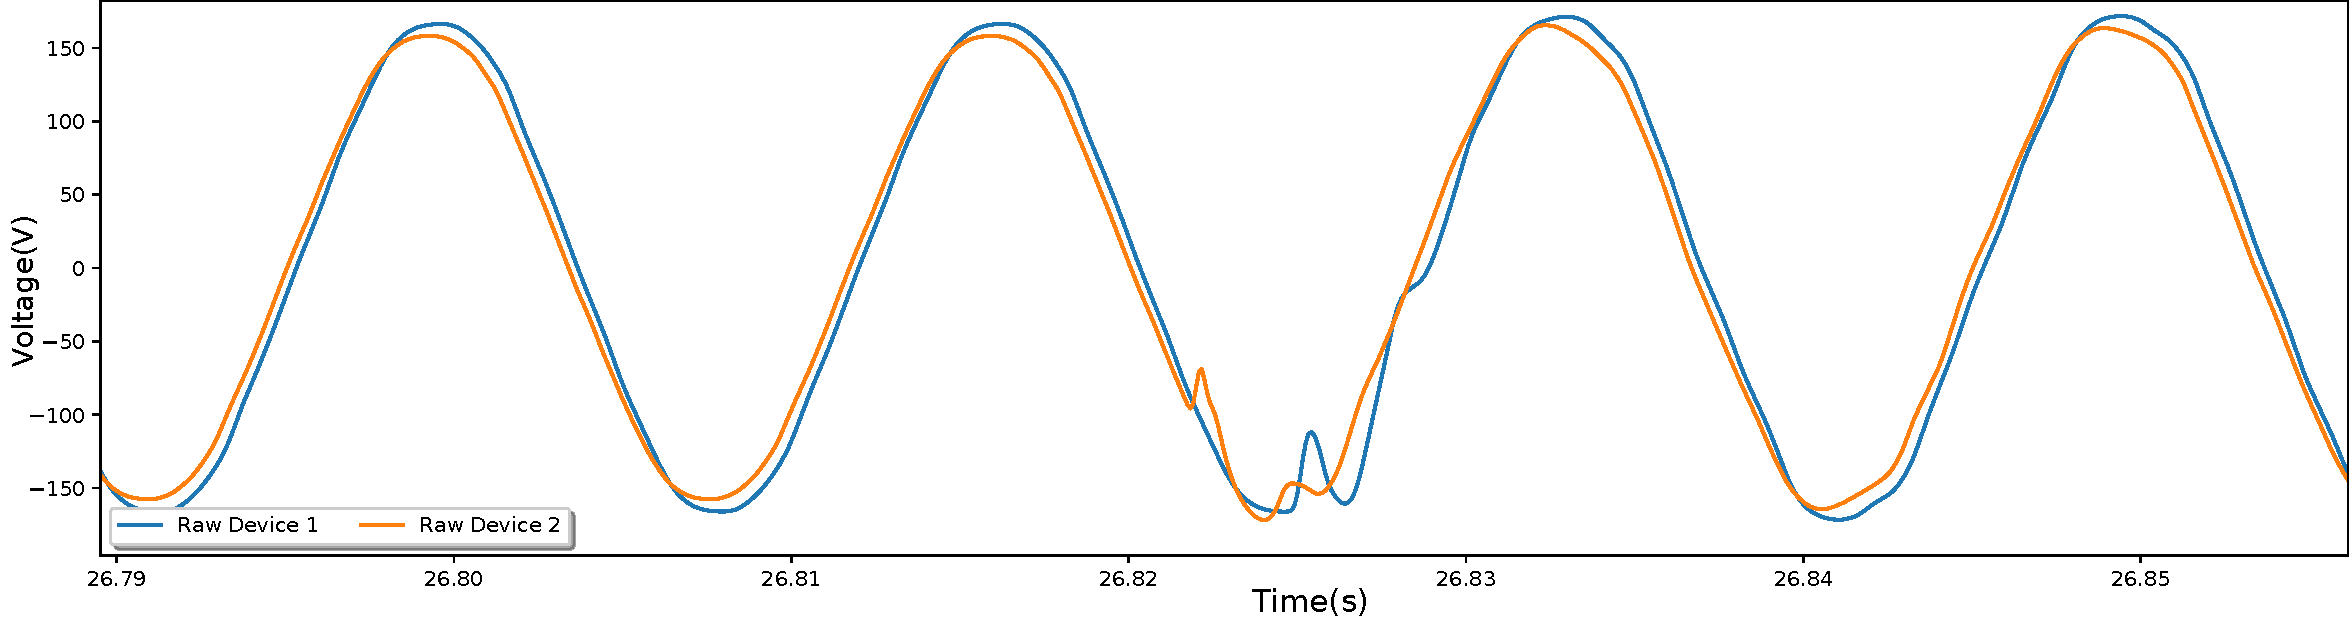
\includegraphics[width=1\linewidth]{img/napali_eval/raw_gridwide_subthreshold_zoom.pdf}
        \caption{}
        \label{fig:expdes:8:2}
    \end{subfigure}
    \caption{Partial sub-threshold event a) the sub-threshold component of the event, b) above threshold component of the event}
    \label{fig:expdes:8}
\end{figure}

An example of a partial sub-threshold event is shown in Figure \ref{fig:expdes:8}.
Figure \ref{fig:expdes:8:1} shows the sub-threshold component of the event.
In this event device 2 passed the threshold on $V_{rms}$ metric, initiating Napali to look for sub-threshold events across other devices.
It is important to note, that at the event start device 1 was considered to be a sub-threshold candidate, however, at $t \approx 26.8s$ device 1 produced a transient metric which was above napali threshold.
As such Napali requested raw data from both device 1 and device 2, creating a partial sub-threshold event containing both a voltage sag shown in Figure \ref{fig:expdes:8:1} and a transient shown in Figure \ref{fig:expdes:8:2}.

\begin{figure}[h]
    \centering
    \begin{subfigure}{0.49\textwidth}
        \centering
        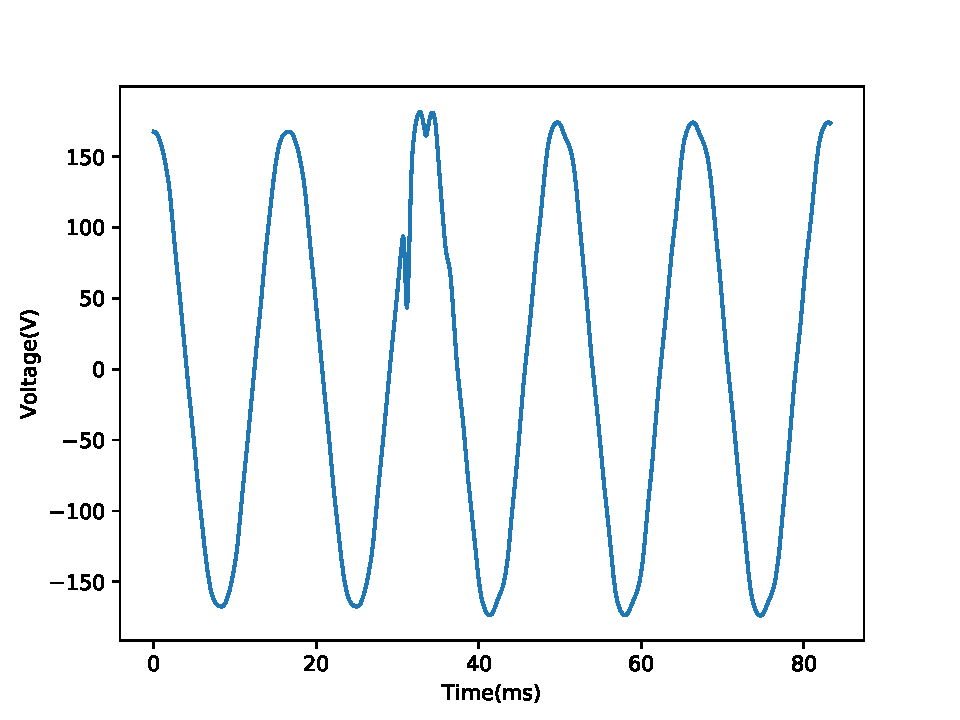
\includegraphics[width=1\linewidth]{img/napali_eval/raw_gridwide_sub_full1.pdf}
        \caption{}
        \label{fig:expdes:9:1}
    \end{subfigure}%
    \begin{subfigure}{0.49\textwidth}
        \centering
        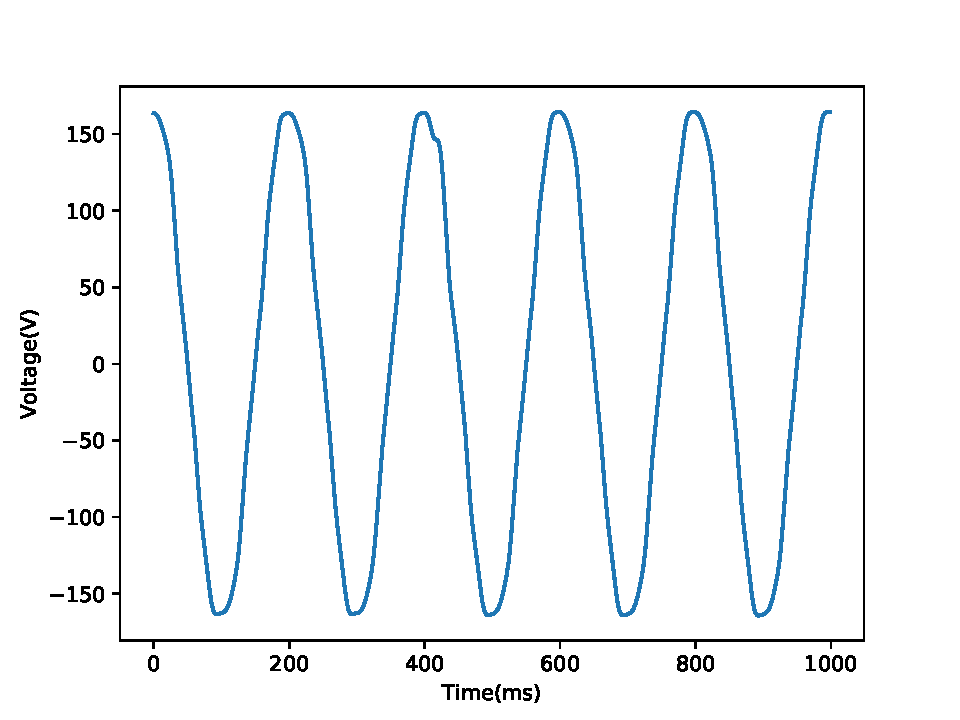
\includegraphics[width=1\linewidth]{img/napali_eval/raw_gridwide_sub_full2.pdf}
        \caption{}
        \label{fig:expdes:9:2}
    \end{subfigure}

    \begin{subfigure}{0.49\textwidth}
        \centering
        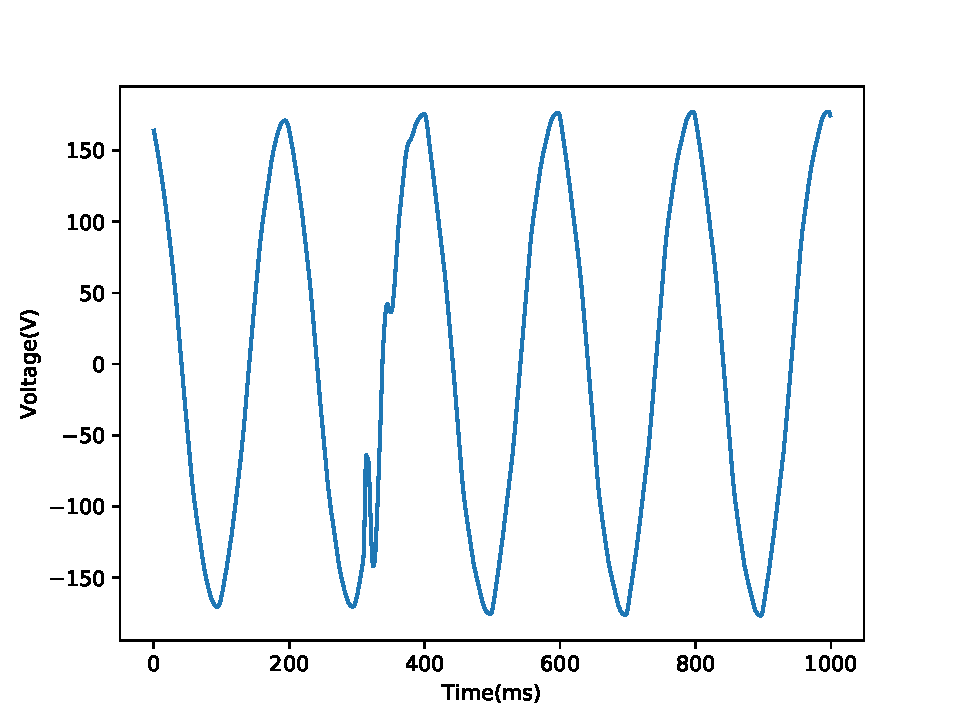
\includegraphics[width=1\linewidth]{img/napali_eval/raw_gridwide_sub_full3.pdf}
        \caption{}
        \label{fig:expdes:9:3}
    \end{subfigure}
    \begin{subfigure}{0.49\textwidth}
        \centering
        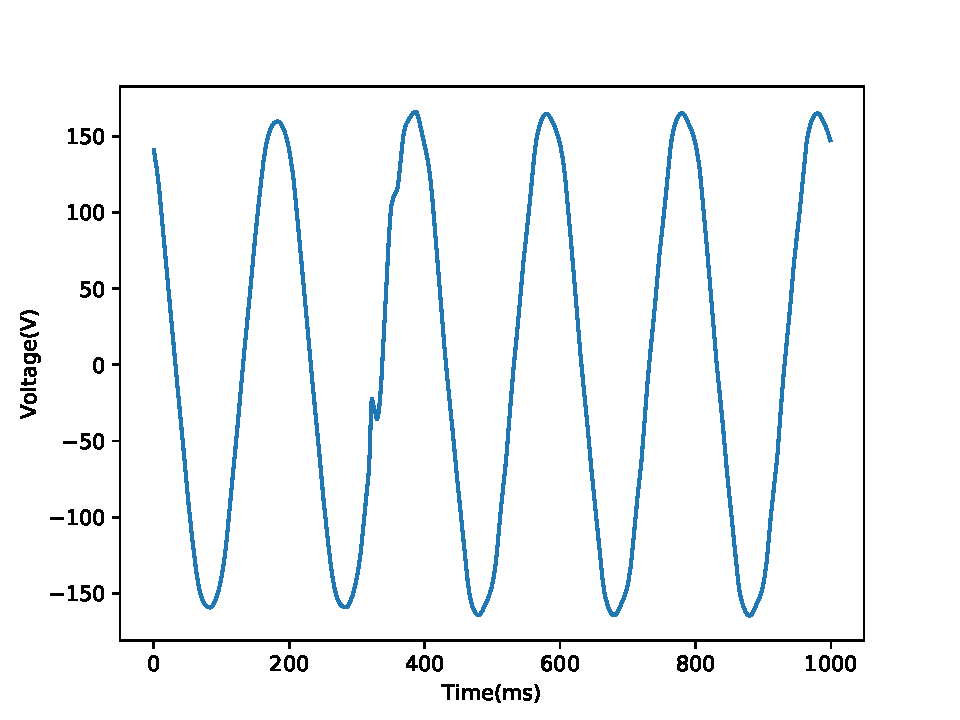
\includegraphics[width=1\linewidth]{img/napali_eval/raw_gridwide_sub_full4.pdf}
        \caption{}
        \label{fig:expdes:9:4}
    \end{subfigure}
    \caption{Full sub-threshold event across 4 devices.
    a) Device 1: above threshold b) Device 2: sub-threshold c) Device 3: above threshold d) Device 4: above threshold.}
    \label{fig:expdes:9}
\end{figure}

An example of a full sub-threshold event is shown in Figure \ref{fig:expdes:9}.
This is a short-lived transient event observed by four devices on September 5\textsuperscript{th}.
Devices 1, 3, and 4 generated a transient metric higher then the Napali threshold.
Device 2 transient metric did not pass threshold, yet nonetheless produced a severe enough deviation from the mean for Napali to consider it a part of the event.
This is particularly evident in the mild transient observed in Figure \ref{fig:expdes:9:2}.

\section{University of Hawaii Deployment.}\label{sec:university-of-hawaii-deployment.}

As part of the Napali validation, the OPQ system was deployed across the University of Hawaii Manoa campus (UH).
This location was ideal because it is an isolated microgrid connected to the Oahu powergrid only via a single 46kV feeder as shown in Figure~\ref{expdes:fig:1}.
Another advantage of the UH campus is the high number of smart meters deployed across various levels of the power delivery infrastructure.
While the purpose of these meters is monitoring the power consumption, they do include some rudimentary power quality monitoring capabilities.
Data from the campus deployed meters was used as ground truth for comparison against the measurements, and analysis performed by the OPQ project.
The location of smart meters in the grid topology is shown in figure~\ref{expdes:fig:1} as the $M$ nodes.
As evident by the meter location none of them were monitoring the consumer level power and mainly focused on the higher voltage power delivery.
This placement was a consequence of the smart meters role as a consumption monitor, and thus the deployment of the OPQ Boxes at the residential level complimented UH power quality monitoring capabilities without introducing redundancies.
University of Hawaii power grid is supplying a highly diverse infrastructure.
Beyond the traditional residential equipment such as computers and consumer grade electronics, the UH power grid powers scientific and laboratory equipment, machine shops, and server farms.
All of these elements have varying requirements/tolerances for power quality anomalies as well as different levels of power quality ``pollution''.
Furthermore, some of the electricity consumers in the UH campus are entirely unique.
For example, the free electron laser located in the Watanabe Hall is one of the only free electron lasers in the world, and the impact/sensitivity of power quality on the instrument are completely unstudied.
\begin{figure}[h]
    \centering
    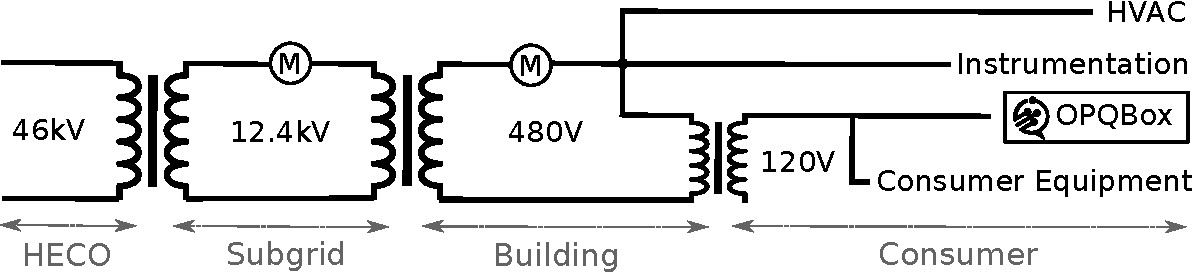
\includegraphics[width=1\linewidth]{img/uh-grid.pdf}
    \caption{University of Hawaii at Manoa power delivery infrastructure.}
    \label{expdes:fig:1}
\end{figure}

There were 74 smart meters deployed across the UH campus.
These meters measured the fundamental frequency $V_{rms}$, power consumption, reactive power, and power factor.
Data from these meters was cross-referenced with the Napali detection system in order to ascertain it's benefits.

OPQ Box placement was specifically selected to cover as much of the University of Hawaii power delivery infrastructure as possible.
The OPQ Box deployment is shown in Figure \ref{expdes:fig:deploy}.
By spreading out devices across the entire power grid, OPQ system is able to monitor the propagation of power quality disturbances throughout the UH power grid.
Consider the event shown in Figure \ref{fig:expdes:9}.
Figure \ref{expdes:fig:grid_wide_filtered} shows the same event with the fundamental and harmonics suppressed using a notch filter bank.
Furthermore, the location annotation is added to indicate the device location.
The most affected devices were located at the Physical Plant and Hamilton Library, recording a $~60V_{pp}$ transient.
Incidentally, both of these devices are monitoring a subgrid rooted at transformer(MA4).
Another device recorded this event was located in Watanabe Hall.
This device recorded a $30V_{pp}$ transient, still above the threshold for detection.
This device was monitoring the the subgrid rooted at the transformer LA4.
The final device was located at the parking structure entirely across campus.
This device recorded a $15V_{pp}$ transient, about 1V below the required magnitude for the threhold based detection.
However, Napali was able to determine that the parking structure OPQ Box was affected by the disturbance, and requested the raw data regardless.

\begin{figure}[h]
    \centering
    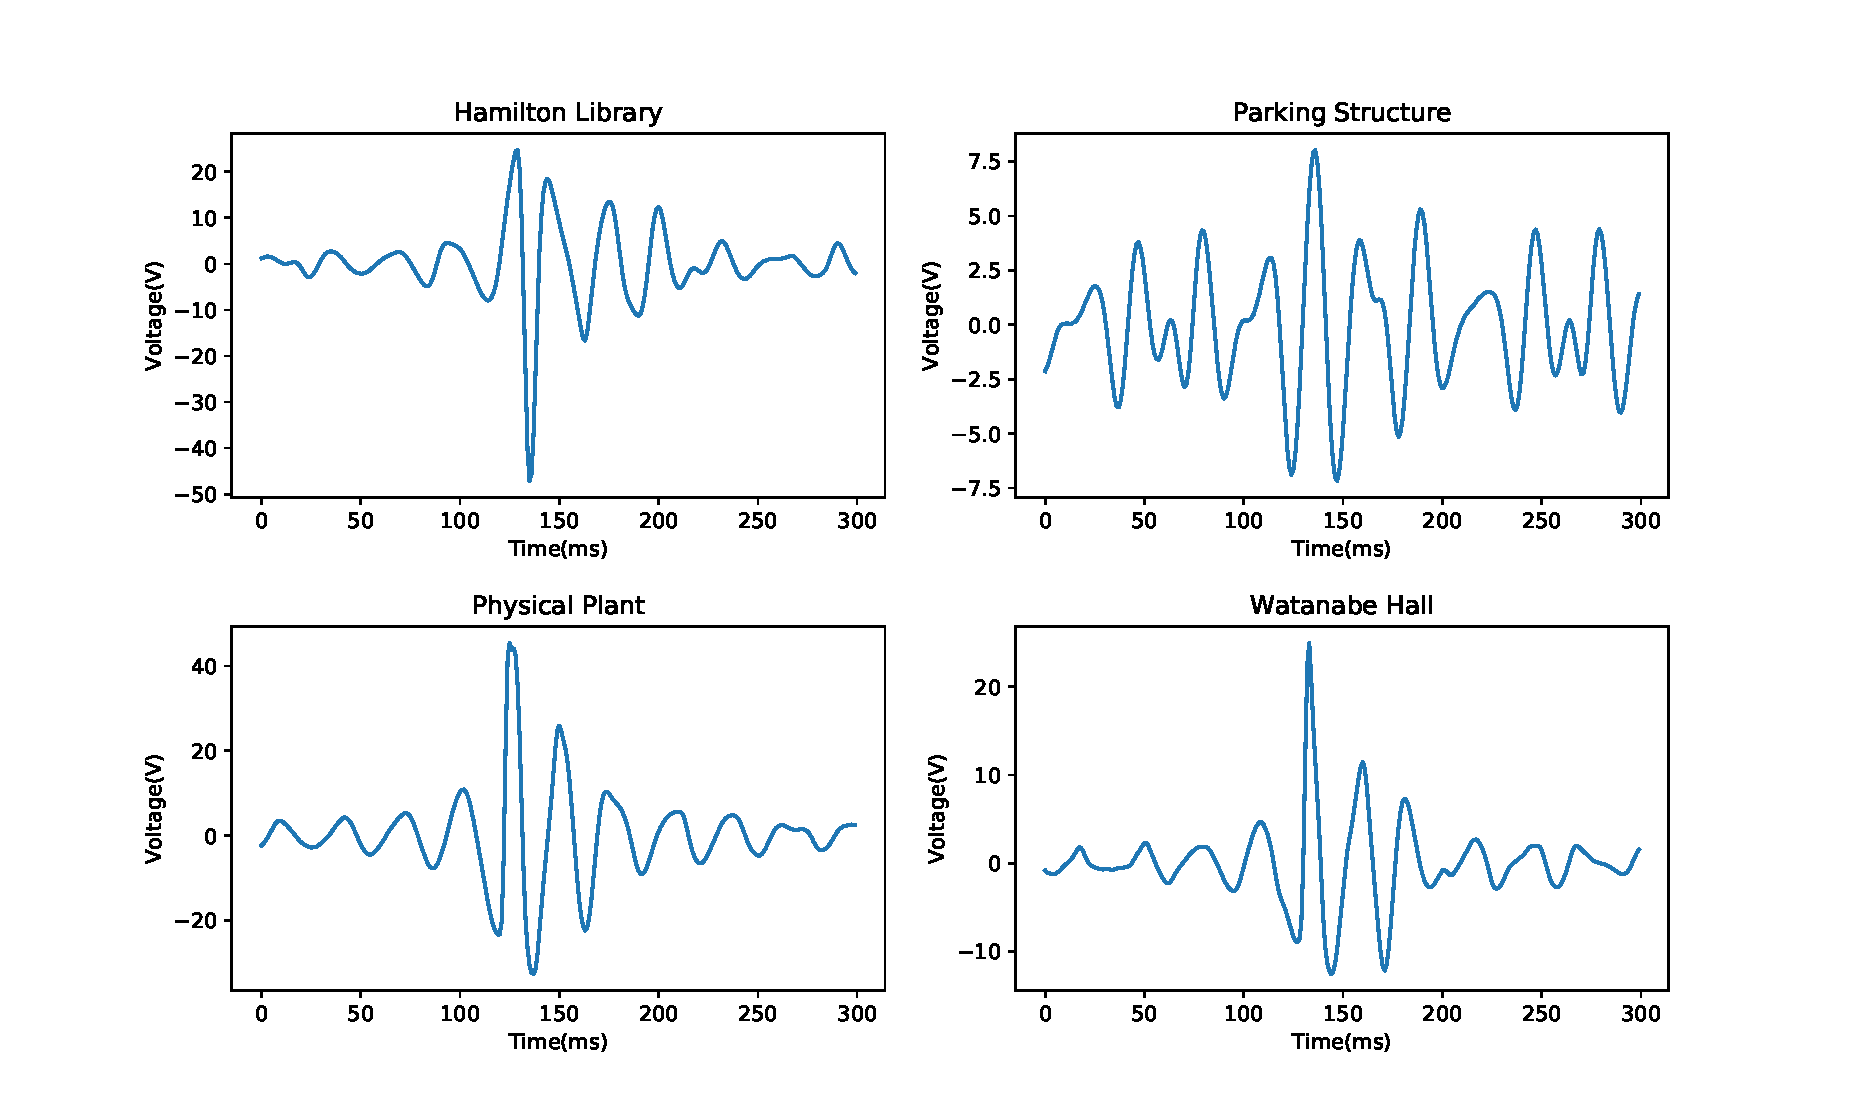
\includegraphics[width=1\linewidth]{img/deployment/gridwide_locality.pdf}
    \caption{Filtered Transient from event shown in Figure \ref{fig:expdes:9}}
    \label{expdes:fig:grid_wide_filtered}
\end{figure}

From the data gathered by Napali as shown in Figure \ref{expdes:fig:grid_wide_filtered}, it seems apparent that the disturbance originated at the subgrid rooted at the transformer MA4.
The Watanabe device was affected due to the short geographic and electrical distance to the MA4 subgrid.
By the time transient reached the parking structure, it was significantly attenuated by the transformers and transmission lines.
It was only detected due to the sub-threshold detection ability of the Napali framework.
\clearpage
\begin{figure}[h]
    \centering
    \includegraphics[width=0.7\linewidth]{img/deployment/uh_power_grid.pdf}
    \caption{OPQ Box locations and device IDs across University of Hawaii.}
    \label{expdes:fig:deploy}
\end{figure}

\clearpage

\subsection{Napali Bandwidth usage} \label{iexp:sec:band}
During the OPQ deployment It was found that Napali significantly outperformed both the self-triggered and the Naive event detection methods.
In order to evaluate the bandwidth performance of Napali a self-triggered plugin was ran along side it inside the Makai host.
This plugin utilized the same thresholds as Napali as described in Table \ref{tbl:opq:thresholds}.
However the self-triggered plugin did not take into the account any inter-device signatures.
This method is equivalent to each the device performing non-collaborative triggering.
\begin{figure}[h]
    \centering
    \includegraphics[width=0.8\linewidth]{img/napali_eval/napali_request_bandwidth.pdf}
    \caption{Amount of data requested from 10 OPQ Boxes via the self-triggered and Napali methods.}
    \label{expdes:fig:self_triggered_bandwidth}
\end{figure}

Figure \ref{expdes:fig:self_triggered_bandwidth} shows the amount of data requested from 10 devices by the self-triggered and Napali plugins over 24 Hours.
It is evident, that the majority of data requests for the self-triggered method resulted in local noise, and did not contribute to the grid measurements.
Napali on the other hand, ignored anomalies which did not affect more then a single device, while requesting sub-threshold data during a gridwide PQ event.

\begin{figure}[h]
    \centering
    \begin{subfigure}{.5\textwidth}
        \centering
        \includegraphics[width=1\linewidth]{img/napali_eval/napali_metric_bandwidth.pdf}
        \caption{}
        \label{expdes:fig:napali_metric_bandwidth}
    \end{subfigure}%
    \begin{subfigure}{.5\textwidth}
        \centering
        \includegraphics[width=1\linewidth]{img/napali_eval/napali_cmd_bandwidth.pdf}
        \caption{}
        \label{expdes:fig:napali_cmd_bandwidth}
    \end{subfigure}
    \caption{Penalties incurred by the Napali framework.
    a) Metrics received from 10 OPQ Boxes.
    b) Commands sent to 10 OPQ Box }
    \label{expdes:fig:napali_bandwidth_penalty}
\end{figure}

It should be noted that the self-triggered method does not incur the penalty of having to constantly transmit the device metrics to the sink, since all the event detection is performed on the device.
Figure \ref{expdes:fig:napali_metric_bandwidth} shows the amount of data received via metrics from 10 OPQ Boxes during the same 24 hours as the Figure \ref{expdes:fig:self_triggered_bandwidth}.
As expected the bandwidth requirement for metric transmission remains constant, since all OPQ Boxes send the metrics at fixed intervals.
While this penalty is significant as it constitutes 41\% of the total bandwidth used by Napali, the aggregate bandwidth is still shows a 440\% improvement over the self-triggered method.
Another penalty incurred by Napali is the two way communication requirement.
Each device which participated the event detection needed to receive a command with the temporal range which anomalous data.
Neither the naive nor self-triggered methods require two-way communication, and as such there is no direct comparison to Napali.
Figure \ref{expdes:fig:napali_cmd_bandwidth} shows the command bandwidth consumption for 10 OPQ Boxes across 24 hours.
The total consumption was ~50kB, which is quite trivial for any modern sensor network.

During the 24 hours of shown in Figures \ref{expdes:fig:napali_bandwidth_penalty} and \ref{expdes:fig:self_triggered_bandwidth}, Napali captured 60 events, while the self-triggered method captured 878.
The average length of the Napali Event was 10s to the self-triggered 3s.
Of 60 Napali events, all 60 contained sub-threshold data.

Comparison of Napali with the naive method was performed analytically.
Since the sampling rate of the OPQ Box is well characterized, and the number of OPQ Boxes is fixed, it is trivial to calculate the amount of raw data generated by the OPQ network during any time period.
In order to make this comparison fair, the raw data bandwidth will be scaled by the compression ratio of the state of the art compression algorithm specifically designed for power quality measurements.\cite{zhang2009new}
Operating at 12kSps, OPQ Box produces raw data at 24KB/s.
With state of the art compression operating at 90\% compression ratio and 5\% overhead of meta-data, one can expect a ~3KB/s stream of raw data for each OPQ box if it were to send the entirety of it to the sink.
For 10 OPQ Boxes we would expect the aggregate bandwidth of 30kB/s, and as such the bandwidth consumption 24.7GB/day.
During a 24 hour period, as shown in Figures \ref{expdes:fig:napali_bandwidth_penalty} and \ref{expdes:fig:self_triggered_bandwidth}, Napali used 234MB of bandwidth.
This corresponds to an over 100x improvement over the naive method.

\begin{figure}[h]
    \centering
    \includegraphics[width=0.8\linewidth]{img/napali_eval/napali_bandwidth_comparison.pdf}
    \caption{Bandwidth requirement comparison between three event detection methods.}
    \label{expdes:fig:bandwidth_master_comparison}
\end{figure}

Figure \ref{expdes:fig:bandwidth_master_comparison} shows the comparison between Napali as well as the naive and self-triggered methods.
While Napali incurs additional costs described in Figure \ref{expdes:fig:napali_bandwidth_penalty} it outperforms the comparable methods.
Finally, the cost of the two way communication as shown in Figure \ref{expdes:fig:napali_cmd_bandwidth} is greatly outweighed by the bandwidth savings in the raw data reception.
Modern sensor networks greatly benefit from two way communication, as it allows on-demand health monitoring, and software updates.
With addition of Napali, two way communication allows for significant bandwidth requirement reduction in for the sensor network as a whole.

\subsection{Sink processing requirement under the Napali Framework} \label{iexp:sec:scale}
Sink processing requirements for event detection between self-triggered, Naive and Napali are quite different.
In general the processing requirement can be described as follows:
\begin{equation}\label{eq:detection_cost}
\begin{aligned}
    C_{total} = C_{metric\_extraction} + C_{detection}
\end{aligned}
\end{equation}

In the Equation \ref{eq:detection_cost} the $C_{total}$ is the total cost, $C_{metric\_extraction}$ is the cost of extracting metrics and $C_{detection}$ is the cost of event detection.\cite{de2015effective}
Each of the three methods, Napali, self triggered, and Naive, has different sink costs associated with each parameter.

First, lets consider the Naive method.
In this case all of the metrics need to be extracted at the sink.
Disregarding the processing power required to keep up with the data rate described in Section \ref{iexp:sec:band} the $C_{feature\_extraction}$ can be measured imperially.
In order perform this measurement OPQ Box software was build for an x86 architecture and stress-tested.
Instead of acquiring data from a device driver, the feature extraction stack was supplied with synthetic data.
Finally the ZMQ communication was removed and replaced with the performance analysis code.
Stress test was performed on a Intel Core i9-8950HK CPU with thermal management disabled running at 2.9GHz.
Under such conditions, the metric extraction stack was able to extract features from 1s worth of raw data in $800us$ running on a single core.
Since metric extraction has no inter-device data dependencies, a modern 8 core CPU we can expect to be able to extract features from 1000 devices.
If an OPQ Box sensor is used with 16 bit samples and 12kSps ADC, aggregate bandwidth for such system is 10.8Gbps, which is well within the realm of a collocated server with dual 10Gbps network interfaces.
$C_{detection}$ cost can be made linear with the number of devices.
If a rolling window is applied to metrics as they are generated.
Raw data from all devices contained in the window with an offending threshold metric can be retained for later analysis.
While simple, this method will collect all of the gridwide events along with a large number of false positives.
In synthetic benchmarks, the $C_{detection}$ made up less then $0.01\%$ of the computational cost when compared to $C_{feature\_extraction}$
and does not significantly contribute to the $C_{total}$.


In contrast to the Naive method, the self triggered method, has no sink processing requirements, since all of the feature-extraction is performed on the edge device.
Thus, self triggered method event detection is only limited by the available network bandwidth.

Napali, being a hybrid of Naive and self triggered methods, moves the $C_{metric\_extraction}$ cost to the edge devices, while retaining
the $C_{detection}$ at the sink.
Unlike the Naive case, napali perform additional computations on the features in order to detect sub-threshold events while excluding the local noise.
However, even with additional metric analysis the Napali stack was able to process synthetic data from 100000 devices on a single core of an a Intel Core i9-8950HK CPU.
This will allow a single server running Makai to provide 50\% coverage of households in the city of Honolulu.

The final step of any power quality analysis stack is event classification.
Every event collected by an event detection system must be analyzed and classified according to their severity and type.
While Makai/Napali are not responsible for event classification it is important to consider the event classification cost when discussing sink processing requirements.
In the case of the Naive method, events which are detected are a mix of local and global events.
However, every event will contain a waveform from every device on the network.
For the self triggered method, only the events which cross the threshold will be considered for classification.
While self triggered events will not contain false positives and sub-threshold events, vast majority of acquired waveforms are comprised of of local disturbances.
Finally, Napali produces high quality events which only contain high fidelity sub and over threshold events, while ignoring local disturbances.
During the campus deployment Napali detected 302 Events comprised of 1561 individual device waveforms a week on average.
The self triggered method detected 26520 offending waveforms.
If we assume unitary classification cost, classification computational requirements for one week of data are shown in Figure \ref{expdes:fig:classification}.
\begin{figure}[h]
    \centering
    \includegraphics[width=0.8\linewidth]{img/napali_eval/classification_cost.pdf}
    \caption{Classification cost based on the expected amount of waveforms for the three considered methods.}
    \label{expdes:fig:classification}
\end{figure}


\subsection{Effects of latency in the Napali framework} \label{iexp:sec:lat}

\begin{figure}[h]
    \centering
    \begin{subfigure}{.45\textwidth}
        \centering
        \includegraphics[width=1\linewidth]{img/napali_eval/event_length.pdf}
        \caption{}
        \label{expdes:fig:event_length}
    \end{subfigure}%
    \begin{subfigure}{.45\textwidth}
        \centering
        \includegraphics[width=1\linewidth]{img/napali_eval/latency.pdf}
        \caption{}
        \label{expdes:fig:latency}
    \end{subfigure}
    \caption{Event length(a) and message latency(b) observed by the OPQ devices.}

    \label{expdes:fig:el_la}
\end{figure}


The latency of Napali triggering system has a significant impact on its ability to read out complete raw data events.
Using generated distributed events as a baseline, I will be able to tune the threshold and temporal requirements for Makai detection algorithms.
Furthermore, temporal, spacial, and amplitude noise will be injected into the generated datasets, to simulate various uncertainties with regards to data collection, such as local noise, and NTP offset errors.
Taking into the account the detection latency of Makai, if some of the requested data is no longer available on the OPQ Box, only a partial time window will be returned.
These events will be marked as incomplete and their fraction as compared to the total number of events recorded will be used to establish the latency tolerance of the Napali framework.
Synthetic benchmarks will be carried out to establish the latency that the Napali system can incur without losing a portion of the event.
Since this is highly dependent on the amount of storage allocated for the RDRB, these experiments will be carried out with various RDRB settings.

Because OPQ Boxes operate using public University of Hawaii WIFI, the latency figures for data transmission are expected to be very dynamic.
In situations with large network contention, greater then 100ms one way packet latency can be expected.
This latency is exacerbated since at least three separate communication steps are required before raw data is received by Makai.
First the metric has to be sent to Makai, next if Makai detects an event, a data request needs to be sent to the affected boxes.
Finally boxes will forward raw data to the Makai sink.
I expect that with RDRB capacity of storing 5 seconds of raw data, no raw data events of 1s or shorter will be missed.
This figure allows for 1 second of transfer latency, 3 seconds of Makai analysis latency, and leaves 1 second of data in RDRB for readout.
However, these figures can only be validated in a real world situations.

\subsection{Temporal locality triggering of the Napali framework} \label{iexp:sec:loc}
Once the OPQ Box is fully validated and the Makai detection thresholds are tuned using synthetic datasets, the Napali system will be fully deployed at the University of Hawaii at Manoa.
 Every time the Napali detects an event, both OPQ Boxes and building meters will be queried for data.
 While it may be unfeasible to query raw data from the UH metering infrastructure, metrics are readily available.
 This data will be used to ascertain the proportion of false positive events detected by Napali.
 Additionally, the internal single point fault detection mechanism of the UH power meters will be used in conjunction with the events detected by Napali to measure the rate of false negative events.
 Both the false negative and false positive measurements will be used to ascertain the detection efficient of the Napali framework.
 This analysis will also include an evaluation  of Napali's ability to reject single point anomalies.
 For a portion of OPQ deployment, every event triggered by a single device will be captured.
 These events will be analyzed in order to determine if a gridwide anomaly was incorrectly classified as a single point disturbance.

The goal of Napali is not to to provide a zero false positive rate.
Once raw data is stored, higher level processing can further filter and classify it using more computationally expensive techniques.
As long as the bandwidth consumption of Napali compares favorably to sending the entirety of raw data to the sink, any rate of false positives can be tolerated.
False negatives on the other hand are the primary metric subject to optimization.
Ideally a zero rate of false positives would be expected, however as with any real-world system I do not expect that to be the case.
This evaluation will determine the triggering efficiency of the Napali framework when compared to the detection ability of a commercially available system.

\subsection{Sub-threshold Data Acquisition} \label{iexp:sec:sub}
The Napali methodology will be compared with the single point anomaly detection approach.
In order to do that I will compare the extent to which sub-threshold events are missed by the UH metering infrastructure.
In a large distributed event, if a portion of events are not detected by the UH meter's single point detection, but picked up by the Napali framework, these events will be flagged and analyzed for their merit.
This will in turn provide a metric of distributed detection ability of the Napali framework compared to commercial system.
Furthermore, for a portion of the deployment the triggering stream from the OPQ Boxes will be stored along with the acquired raw data.
The triggering stream can be used to compute which fraction of devices would have self triggered if operating autonomously.
This will provide the baseline for sub-threshold triggering efficiency of the Napali system, with respect to the single point detection ability of the OPQ Box.

This evaluation will compare Napali performance to the single point detection mechanisms currently in deployment.
I expect that Napali will outperform these strategies, and provide a more complete picture of gridwide anomalies as they propagate through the UH power grid.
It is possible that no sub-threshold events will be recorded during the UH deployment.
UH campus is quite small, perhaps too small for an anomaly in one building not to impact the rest of campus.
In this case the sub-threshold data acquisition will remain an open topic for future work and a larger geographical deployment.
Regardless, as long as I am be able to validate the single point anomaly rejection ability of Napali as described in Section~\ref{iexp:sec:loc}, I will be able to conclude that Napali has a distinct advantage over single point detection methods.
Single point anomalies are not important in smart grid monitoring, since they originate from the consumers side of the meter, and should be ignored.
In fact, recording these events may be detrimental to the privacy of the end-user, since it may give clues on their activities as shown in Figure~\ref{intro:fig:1} a and b.
However since privacy implication of power quality monitoring are outside the scope of this project, this study will remain as a point of future work.




\bibliography{dissertation.bib}
\bibliographystyle{plain}
  
\end{document}
